% README del proyecto en LaTeX
\documentclass[11pt,a4paper]{article}
\usepackage[spanish, es-tabla]{babel}
\usepackage[utf8]{inputenc}
\usepackage{geometry}
\usepackage{amsmath}
\usepackage{hyperref}
\hypersetup{hidelinks}
\usepackage{graphicx}
\usepackage{xcolor}
\usepackage{float}
\usepackage{tabularx}
\usepackage{booktabs}
\usepackage{pgfgantt}
\usepackage{pdflscape}
\usepackage{float}
\usepackage{graphicx}
\usepackage{tikz}
\usetikzlibrary{
    babel,
    arrows.meta,
    positioning,
    shapes.geometric,
    shapes.misc,
    fit,
    calc
}



% === PREÁMBULO SEGURO PARA EVITAR ERRORES ===
\usetikzlibrary{shapes,arrows}

\tikzstyle{block} = [rectangle, draw, rounded corners,
                     minimum width=3cm, minimum height=1cm,
                     align=center]
\tikzstyle{arrow} = [->, thick]


\geometry{margin=2.5cm}

\title{ \textbf{ 
Generación y Adquisición de Señal Senoidal en STM32G474RE} \\
\large Grado en Ingeniería Informática \\ Universidad de Sevilla 
}
\author{Autor: Rafael García Ruiz \\ \small Director: Pablo Pérez García}
\date{2025/2026}

\usepackage{color}
\usepackage{listings}
\definecolor{GrayCodeBlock}{RGB}{241,241,241}
\definecolor{BlackText}{RGB}{110,107,94}
\definecolor{RedTypename}{RGB}{182,86,17}
\definecolor{GreenString}{RGB}{96,172,57}
\definecolor{PurpleKeyword}{RGB}{184,84,212}
\definecolor{GrayComment}{RGB}{170,170,170}
\definecolor{GoldDocumentation}{RGB}{180,165,45}
\lstdefinelanguage{rust}
{
    columns=fullflexible,
    keepspaces=true,
    frame=single,
    framesep=0pt,
    framerule=0pt,
    framexleftmargin=4pt,
    framexrightmargin=4pt,
    framextopmargin=5pt,
    framexbottommargin=3pt,
    xleftmargin=4pt,
    xrightmargin=4pt,
    backgroundcolor=\color{GrayCodeBlock},
    basicstyle=\ttfamily\color{BlackText},
    keywords={
        true,false,
        unsafe,async,await,move,
        use,pub,crate,super,self,mod,
        struct,enum,fn,const,static,let,mut,ref,type,impl,dyn,trait,where,as,
        break,continue,if,else,while,for,loop,match,return,yield,in
    },
    keywordstyle=\color{PurpleKeyword},
    ndkeywords={
        bool,u8,u16,u32,u64,u128,i8,i16,i32,i64,i128,char,str,
        Self,Option,Some,None,Result,Ok,Err,String,Box,Vec,Rc,Arc,Cell,RefCell,HashMap,BTreeMap,
        macro_rules
    },
    ndkeywordstyle=\color{RedTypename},
    comment=[l][\color{GrayComment}\slshape]{//},
    morecomment=[s][\color{GrayComment}\slshape]{/*}{*/},
    morecomment=[l][\color{GoldDocumentation}\slshape]{///},
    morecomment=[s][\color{GoldDocumentation}\slshape]{/*!}{*/},
    morecomment=[l][\color{GoldDocumentation}\slshape]{//!},
    morecomment=[s][\color{RedTypename}]{\#![}{]},
    morecomment=[s][\color{RedTypename}]{\#[}{]},
    stringstyle=\color{GreenString},
    string=[b]"
}
\newcommand{\myparagraph}[1]{\paragraph{#1}\mbox{}\\}
\newcommand{\mysubparagraph}[1]{\subparagraph{#1}\mbox{}\\}


\begin{document}
\maketitle

\begin{figure}[!t]
    \centering
    
\includegraphics[width=\linewidth]{uslogo.png}
\end{figure}
\newpage

\section*{Resumen}
\addcontentsline{toc}{section}{Resumen}

El presente Trabajo de Fin de Grado aborda el diseño y desarrollo de un sistema embebido para la generación y adquisición de señales senoidales aplicado al estudio de impedancias. El sistema se implementa sobre el microcontrolador \textbf{STM32G474RE}, aprovechando sus periféricos internos con el objetivo de reducir la necesidad de componentes externos y obtener una solución compacta, eficiente y de bajo coste.

El funcionamiento del dispositivo se basa en la generación de una señal senoidal mediante el convertidor digital-analógico (\textbf{DAC}) del microcontrolador. Dicha señal se obtiene a partir de una tabla de muestras precalculada y se transmite al periférico mediante \textbf{DMA}, utilizando un temporizador interno como fuente de disparo para garantizar una frecuencia de actualización estable. La señal generada se aplica posteriormente a una muestra o carga de prueba, cuya respuesta es adquirida mediante el convertidor analógico-digital (\textbf{ADC}), también asistido por DMA.

Una parte fundamental del proyecto consiste en la sincronización entre la generación y la adquisición de la señal. Para ello se emplea el temporizador \textbf{TIM6}, que permite coordinar el funcionamiento del DAC y del ADC mediante eventos hardware, reduciendo la intervención de la CPU y minimizando posibles errores derivados de la latencia del software.

El firmware del sistema se desarrolla en \textbf{Rust} en un entorno \textit{bare-metal}, sin sistema operativo ni biblioteca estándar. Esta elección permite explorar el uso de un lenguaje moderno en sistemas embebidos, destacando sus ventajas en cuanto a seguridad de memoria, control de recursos y robustez del código. Durante el desarrollo se configura una infraestructura completa de compilación cruzada, carga y depuración mediante herramientas como \texttt{Cargo}, \texttt{probe-rs} y \texttt{defmt}.

Finalmente, el sistema se valida mediante pruebas experimentales orientadas a comprobar la correcta generación de la señal senoidal, la adquisición de muestras mediante el ADC y la estabilidad del funcionamiento basado en DMA. El proyecto demuestra la viabilidad de utilizar el STM32G474RE con Rust como plataforma integrada para aplicaciones de generación, adquisición y análisis de señales analógicas, sentando las bases para futuros desarrollos relacionados con la caracterización eléctrica de materiales o tejidos biológicos.

\bigskip

\noindent\textbf{Palabras clave:} STM32G474RE, Rust, bare-metal, no-std, bioimpedancia, DAC, ADC, DMA, TIM6, sistemas embebidos, señal senoidal.

\newpage

\tableofcontents
\section*{Glosario de términos y acrónimos}
\addcontentsline{toc}{section}{Glosario de términos y acrónimos}

\begin{description}
    \item[ADC (Analog-to-Digital Converter):] Periférico que convierte una señal analógica de tensión en un valor digital numérico.
    \item[DAC (Digital-to-Analog Converter):] Periférico que convierte un valor numérico digital en una señal de tensión analógica.
    \item[DMA (Direct Memory Access):] Mecanismo que permite a los periféricos acceder a la memoria RAM independientemente de la CPU, reduciendo la carga de procesamiento.
    \item[HAL (Hardware Abstraction Layer):] Capa de software que permite interactuar con el hardware del microcontrolador sin necesidad de manipular registros directamente.
    \item[Impedancia ($Z$):] Medida de oposición total que presenta un circuito al paso de una corriente alterna.
    \item[Jitter:] Variabilidad temporal en la ejecución de un evento o en la llegada de una señal, crítica en sistemas de tiempo real.
    \item[no\_std:] Atributo de Rust que indica que el programa no utiliza la biblioteca estándar (std), permitiendo su ejecución en sistemas sin sistema operativo (bare-metal).
    \item[Ownership:] Concepto central de Rust que gestiona la seguridad de memoria mediante reglas de propiedad y préstamo de variables.
    \item[PCB (Printed Circuit Board):] Placa de circuito impreso donde se montan y conectan los componentes electrónicos.
    \item[RCC (Reset and Clock Control):] Módulo encargado de gestionar los relojes y el reinicio de los periféricos en el STM32.
    \item[UART (Universal Asynchronous Receiver-Transmitter):] Protocolo de comunicación serie utilizado habitualmente para transmitir datos a un ordenador.
\end{description}
\newpage

\section{Introducción del proyecto}

El análisis de las propiedades eléctricas de los tejidos biológicos, conocido como bioimpedancia, se ha consolidado como una herramienta fundamental en la medicina moderna para la caracterización de estados fisiológicos y patológicos. Sin embargo, el diseño de instrumentación precisa y de bajo coste para este propósito presenta desafíos significativos en la sincronización de señales y en la fiabilidad del software embebido.

El presente Trabajo de Fin de Grado aborda el diseño, desarrollo e implementación de un sistema de adquisición de señales biomédicas basado en el microcontrolador de alto rendimiento \textbf{STM32G474RE}. La propuesta se diferencia de las soluciones tradicionales por el uso del lenguaje de programación \textbf{Rust}, cuya seguridad de memoria y gestión de recursos sin tiempo de ejecución (\textit{no-std}) ofrece una robustez superior para aplicaciones críticas.

\begin{figure}[H]
\centering
\begin{tikzpicture}[node distance=4.5cm]
\node[block] (dac) {DAC};
\node[block, right of=dac] (sample) {Muestra};
\node[block, right of=sample] (adc) {ADC};

\draw[arrow] (dac) -- (sample);
\draw[arrow] (sample) -- (adc);
\end{tikzpicture}
\caption{Diagrama conceptual del sistema}
\end{figure}


\subsection{Resumen de objetivos}

El objetivo del proyecto es desarrollar una plataforma embebida capaz de generar una señal senoidal mediante el DAC del STM32G474RE y adquirir su respuesta mediante el ADC, utilizando Rust como lenguaje de implementación y periféricos internos del microcontrolador para reducir la intervención de la CPU.
\begin{itemize}
    \item \textbf{Desarrollo de un motor de síntesis digital:} Implementar la generación de ondas senoidales mediante el uso coordinado de tablas en memoria, acceso directo a memoria (DMA) y convertidores digital-analógico (DAC).
    \item \textbf{Sincronización de hardware:} Configurar un sistema de disparo (\textit{triggering}) basado en temporizadores para garantizar que la adquisición (ADC) y la generación (DAC) ocurran en fase, eliminando el error por latencia de software.
    \item \textbf{Implementación en Rust embebido:} Explorar y validar el uso de Rust en un entorno \textit{bare-metal}, accediendo a los registros del microcontrolador mediante la capa PAC disponible para la familia STM32G4.
    \item \textbf{Monitorización de muestras:} Establecer un flujo de datos eficiente para observar las muestras adquiridas en tiempo real mediante \texttt{defmt}, RTT y \texttt{probe-rs}.
\end{itemize}

A través de estos objetivos, el proyecto busca demostrar que es posible desarrollar un prototipo funcional de instrumentación embebida utilizando componentes de bajo coste y lenguajes de programación modernos.


\section{Descripción del proyecto}

En este proyecto se aborda el diseño y desarrollo de un sistema de adquisición biomédica basado en un microcontrolador \textbf{STM32G474RE}. Su función principal es generar una señal senoidal controlada mediante el DAC y adquirir la señal resultante mediante el ADC tras atravesar una muestra o carga de prueba. La comparación externa de ambas señales permite observar efectos relacionados con sus propiedades eléctricas, tales como atenuación, filtrado o variaciones de amplitud asociadas a la impedancia.

La coordinación entre generación y adquisición se realiza mediante \textbf{TIM6} y \textbf{DMA}. El temporizador proporciona el evento periódico de disparo, mientras que el DMA transfiere muestras hacia el DAC y desde el ADC sin requerir una intervención continua de la CPU.

El diseño del sistema se inspira en enfoques previamente utilizados en instrumentación biomédica basada en microcontroladores y análisis de señal aplicada al estudio de propiedades tisulares.

El dispositivo se divide en dos bloques funcionales principales:

\begin{itemize}
    \item \textbf{Generación de la señal:} producción de una onda senoidal a partir de una tabla precalculada de 12~bits, transferida al DAC mediante DMA y temporizada por TIM6.

    \item \textbf{Lectura y monitorización:} adquisición sincronizada mediante ADC y almacenamiento de muestras en memoria mediante DMA, con visualización posterior mediante trazas de depuración.
\end{itemize}

Durante el desarrollo del proyecto se busca implementar la mayor parte del sistema utilizando los periféricos internos del microcontrolador, reduciendo la necesidad de componentes externos.

\subsection{Estado del arte}

\subsubsection{Fundamentos teóricos}

\myparagraph{Concepto de impedancia}

La \textbf{impedancia} (\(Z\)) es la medida de la oposición que presenta un circuito al paso de una corriente cuando se aplica una tensión alterna \cite{hayt2012}. Constituye un parámetro fundamental en el análisis de sistemas eléctricos y electrónicos, ya que describe la relación entre el voltaje y la corriente en régimen sinusoidal. Su definición básica es:

\[
Z = \frac{V}{I} \quad [\Omega]
\]

A diferencia de la corriente continua (CC), donde únicamente interviene la resistencia, en corriente alterna (CA) la respuesta del circuito depende también de la \textbf{frecuencia} de la señal. Esto se debe a la presencia de elementos \emph{reactivos} (condensadores e inductancias), que modifican tanto la amplitud como la fase de la corriente respecto al voltaje aplicado.

Por ello, la impedancia combina dos componentes y se expresa como un número complejo:

\[
Z = R + jX \quad [\Omega]
\]

donde:
\begin{itemize}
    \item \(R\) es la parte real, correspondiente a la \textbf{resistencia}, que describe la disipación de energía.
    \item \(X\) es la parte imaginaria, la \textbf{reactancia}, asociada a los efectos capacitivos e inductivos que provocan variaciones en la fase de la corriente.
\end{itemize}

En consecuencia, la impedancia se representa de forma vectorial incorporando tanto magnitud como fase, características esenciales para el análisis de señales sinusoidales.

\myparagraph{Concepto de fasor}

Las señales presentes en los circuitos de corriente alterna suelen ser de naturaleza sinusoidal. Para simplificar su análisis, se emplea la representación mediante \textbf{fasores} \cite{oppenheim2010}, que transforma magnitudes dependientes del tiempo en números complejos de módulo y fase constante.

Una tensión sinusoidal puede expresarse como:

\[
v(t) = V_{\text{max}} \cdot \sin(\omega t)
\]

donde:
\begin{itemize}
    \item \(v(t)\): tensión instantánea.
    \item \(V_{\text{max}}\): amplitud o valor máximo de la señal.
    \item \(\omega t\): argumento o posición angular de la onda, siendo \(\omega\) la frecuencia angular.
\end{itemize}

Los fasores permiten representar esta señal mediante un número complejo cuya:
\begin{itemize}
    \item \textbf{magnitud} se corresponde con la amplitud (o valor eficaz) de la onda,
    \item \textbf{fase} describe el desplazamiento angular respecto a una referencia.
\end{itemize}

Dado que la impedancia también se expresa como un número complejo, la representación fasorial simplifica notablemente el análisis de circuitos en régimen permanente sinusoidal. Por ello constituye una herramienta fundamental para describir impedancias y estudiar el comportamiento eléctrico de materiales, tejidos o componentes electrónicos.

\subsubsection{Medición de la impedancia}

La medición de impedancia es fundamental para analizar y diseñar circuitos eléctricos y electrónicos. Su valor proporciona información clave sobre el comportamiento del sistema ante diferentes frecuencias, especialmente debido a que la impedancia depende de la reactancia, la cual varía con la frecuencia. Por ello, resulta necesario realizar mediciones en un rango adecuado de frecuencias para identificar posibles fallos, optimizar el rendimiento del circuito y evaluar su comportamiento dinámico.

Dado que la impedancia es un valor complejo, su medición requiere instrumentos o técnicas específicas que permitan determinar tanto su magnitud como su fase.

\myparagraph{Generador de señales y osciloscopio}

Una técnica básica de medición consiste en generar una señal conocida, generalmente sinusoidal, mediante un generador de señales. La señal se aplica al componente bajo prueba, observando la respuesta mediante un osciloscopio. Este método permite comparar la amplitud, fase y forma de la señal aplicada con la señal resultante, proporcionando una evaluación cualitativa del comportamiento del circuito.

\myparagraph{Medición LCR o puente de impedancia}

El puente LCR permite medir impedancias con gran precisión. El método compara la impedancia desconocida con elementos de impedancia conocida. Ajustando estos elementos hasta equilibrar el puente, es posible determinar la impedancia del componente bajo prueba con elevada exactitud.

\myparagraph{Medición en dos puntos}

Este método mide la resistencia o impedancia del elemento bajo prueba en serie con una resistencia auxiliar. Se asume que la resistencia auxiliar es despreciable frente a la del elemento medido. Aunque es un método sencillo, puede producir errores si ambas resistencias son comparables. Debido a su simplicidad, este será el método utilizado en nuestro proyecto.

\myparagraph{Medición en tres puntos}

En este caso se utilizan dos resistencias auxiliares adicionales. Se realizan tres mediciones: \(R_{12}\), \(R_{23}\) y \(R_{13}\). La resistencia buscada se calcula mediante:

\[
R_1 = \frac{R_{12} - R_{23} + R_{13}}{2}
\]

Este método mejora la precisión respecto al de dos puntos, aunque puede presentar errores si las resistencias auxiliares son demasiado altas o si no se mantiene una separación adecuada entre puntos de medición.

\myparagraph{Medición en cuatro puntos}

Este método emplea cuatro electrodos: dos para inyectar corriente y dos para medir la caída de tensión. La separación entre los electrodos de corriente y de medida reduce la influencia de las resistencias de contacto, permitiendo una medición precisa. La impedancia se calcula mediante la ley de Ohm:

\[
Z = \frac{V}{I}
\]

\myparagraph{MFIA Impedance Analyzer}

El MFIA es un analizador de impedancias digital de alta precisión que opera entre 1~mHz y 500~kHz, con una exactitud básica del 0.05\%. Su rango de medición abarca desde 1~m\(\Omega\) hasta 1~T\(\Omega\). Sus aplicaciones incluyen ingeniería eléctrica, caracterización de materiales y bioimpedancia.

\myparagraph{Impedimed SFB7}

El dispositivo SFB7 realiza espectroscopia de bioimpedancia tetrapolar a 256 frecuencias entre 4~kHz y 1000~kHz. Emplea modelos como el de Cole y la teoría de mezcla de Hanai para estimar parámetros corporales como TBW, ECF, ICF, FFM y FM, lo que lo convierte en un estándar en estudios biomédicos.

\myparagraph{Keysight E4980A Precision LCR Meter}

El medidor LCR Keysight E4980A es ampliamente utilizado por su capacidad para medir inductancia, capacitancia y resistencia con alta precisión. Opera entre 20~Hz y 2~MHz, con una exactitud básica del 0.05\%, ofreciendo gran estabilidad y repetibilidad en un amplio rango de mediciones.

\begin{figure}[H]
\centering

\shorthandoff{<>}

\begin{tikzpicture}

\def\Rx{3}
\def\Xy{2}

% Ejes
\draw[->] (-0.3,0) -- (4,0) node[right] {$R$};
\draw[->] (0,-0.3) -- (0,3) node[above] {$jX$};

% Vector
\draw[->, thick] (0,0) -- (\Rx,\Xy) node[midway, above] {$Z$};

% Proyecciones
\draw[dashed] (\Rx,0) -- (\Rx,\Xy);
\draw[dashed] (0,\Xy) -- (\Rx,\Xy);

% Etiquetas
\node[below] at (\Rx,0) {$R$};
\node[left] at (0,\Xy) {$X$};

% Ángulo
\draw (0.8,0) arc[start angle=0,end angle={atan(\Xy/\Rx)},radius=0.8];
\node at (1,0.3) {$\phi$};

\end{tikzpicture}

\shorthandon{<>}

\caption{Representación fasorial de la impedancia compleja}
\label{fig:fasor}
\end{figure}


\subsection{Objetivos del proyecto}

El objetivo principal de este proyecto es desarrollar un sistema embebido capaz de generar una señal senoidal, aplicarla a una muestra y medir la señal resultante tras atravesar dicho medio, con el fin de obtener información relacionada con sus propiedades eléctricas. Todo el sistema se implementará sobre el microcontrolador \textbf{STM32G474RE}, aprovechando al máximo sus periféricos internos para minimizar la necesidad de componentes externos.

El dispositivo deberá cumplir las siguientes características fundamentales:

\begin{itemize}
    \item \textbf{Implementación interna}: toda la lógica del sistema y el mayor número posible de funciones deben realizarse mediante los periféricos integrados en el microcontrolador (DAC, ADC, temporizadores, DMA, etc.).
    \item \textbf{Generación y adquisición de señal}: el sistema debe generar una señal senoidal estable y adquirir la señal de salida tras atravesar la muestra o carga de prueba.
    \item \textbf{Configurabilidad}: la frecuencia de la señal generada debe poder ajustarse mediante perfiles predefinidos para permitir ensayos en distintos rangos de operación. La amplitud se mantiene fija en esta versión del prototipo mediante la tabla senoidal empleada por el DAC.
\end{itemize}

Además del objetivo principal, el desarrollo del proyecto permitirá adquirir conocimientos y habilidades en diversas áreas:

\begin{itemize}
    \item \textbf{Microcontroladores}: estudio y configuración del STM32G474RE, programación en Rust y manejo de periféricos como DAC, ADC, temporizadores, GPIO y sistemas de reloj.
    \item \textbf{DMA (Direct Memory Access)}: configuración del DMA para automatizar la transferencia de datos en la generación y adquisición de señal, reduciendo la carga de la CPU y aumentando el rendimiento.
    \item \textbf{Señal analógica}: acondicionamiento externo básico y manejo de señales alternas en el contexto de generación y adquisición con DAC y ADC.
    \item \textbf{Impedancia}: adquisición y análisis de datos para estudiar la impedancia de muestras, interpretación de los resultados y relación con su comportamiento eléctrico.
    \item \textbf{Procesamiento de ondas}: trabajo con señales sinusoidales, tablas de onda, ajuste de frecuencia y análisis externo de las señales adquiridas.
    \item \textbf{Montaje y soldadura}: desarrollo de un prototipo inicial sobre placa perforada, instalación y conexión de componentes externos y verificación del circuito.
    \item \textbf{Conversión CA/CC}: generación de una señal alterna mediante el DAC a partir de una referencia continua, y conversión de la señal resultante nuevamente a valores digitales mediante el ADC.
\end{itemize}

El alcance del proyecto incluye el estudio del estado del arte, el diseño conceptual y electrónico del sistema, la implementación y verificación de un prototipo funcional de laboratorio y la obtención de medidas experimentales con cargas conocidas. El diseño de una versión compacta o de una PCB dedicada queda planteado como una posible línea de continuación.

\section{Planificación del proyecto}
\subsection{Análisis de requisitos}

\myparagraph{R1 – Microcontrolador como núcleo del sistema}
El diseño del sistema debe implementarse empleando el microcontrolador \textbf{STM32G474RE} como elemento principal, utilizando tantos periféricos internos como sea posible con el fin de minimizar la necesidad de componentes externos.

\mysubparagraph{R1.1 – DAC}
El microcontrolador debe disponer de al menos un DAC funcional para generar la señal senoidal inicial que será aplicada a la muestra (requisito R2).

\mysubparagraph{R1.2 – ADC}
El sistema debe contar con un ADC de adecuada resolución y frecuencia de muestreo para medir la señal resultante tras atravesar la muestra. En esta versión del proyecto no es necesaria la presencia de múltiples ADC.

\mysubparagraph{R1.3 – Temporizadores}
El sistema debe contar con al menos un temporizador capaz de controlar tanto la generación de la señal como el disparo del ADC para asegurar una captura sincronizada. En este proyecto se emplea un único temporizador (\textbf{TIM6}) como generador de eventos TRGO.

% ============================================================
% DIAGRAMA 2: SINCRONIZACIÓN TIM6 - DAC - ADC - DMA
% ============================================================

\begin{figure}[H]
\centering
\resizebox{0.95\textwidth}{!}{%
\begin{tikzpicture}[
    signal/.style={thick},
    arrow/.style={-{Latex[length=2.5mm]}, thick},
    label/.style={font=\small},
    ticklabel/.style={font=\scriptsize}
]

% Ejes temporales
\draw[arrow] (0,-0.3) -- (11.5,-0.3) node[right, label]{tiempo};

% Etiquetas
\node[label, anchor=east] at (-0.3,3.2) {TIM6 TRGO};
\node[label, anchor=east] at (-0.3,2.2) {Actualización DAC};
\node[label, anchor=east] at (-0.3,1.2) {Muestreo ADC};
\node[label, anchor=east] at (-0.3,0.2) {Transferencias DMA};

% Señal TIM6 TRGO: pulsos
\foreach \x in {1,3,5,7,9} {
    \draw[signal] (\x,3) -- (\x,3.5) -- (\x+0.25,3.5) -- (\x+0.25,3);
}
\draw[signal] (0.4,3) -- (1,3);
\draw[signal] (1.25,3) -- (3,3);
\draw[signal] (3.25,3) -- (5,3);
\draw[signal] (5.25,3) -- (7,3);
\draw[signal] (7.25,3) -- (9,3);
\draw[signal] (9.25,3) -- (10.8,3);

% Eventos DAC
\foreach \x/\muestra in {1/m0,3/m1,5/m2,7/m3,9/m4} {
    \draw[arrow] (\x+0.12,2.45) -- (\x+0.12,2.0);
    \node[ticklabel] at (\x+0.12,1.75) {\muestra};
}

% Eventos ADC
\foreach \x/\muestra in {1/b0,3/b1,5/b2,7/b3,9/b4} {
    \draw[arrow] (\x+0.12,1.45) -- (\x+0.12,1.0);
    \node[ticklabel] at (\x+0.12,0.75) {\muestra};
}

% DMA
\foreach \x/\txt in {1/DAC$\leftarrow$m0,3/DAC$\leftarrow$m1,5/DAC$\leftarrow$m2,7/ADC$\rightarrow$b3,9/ADC$\rightarrow$b4} {
    \draw[rounded corners, draw] (\x-0.45,-0.15) rectangle (\x+0.75,0.45);
    \node[ticklabel] at (\x+0.15,0.15) {\txt};
}

% Indicaciones de periodo
\draw[arrow, thin] (1.12,3.85) -- (3.12,3.85);
\node[ticklabel] at (2.12,4.1) {$T_{trigger}$};

\node[ticklabel] at (5.12,-0.95) {Secuencia circular de muestras};

\end{tikzpicture}%
}
\caption{Sincronización entre TIM6, DAC, ADC y DMA. Cada evento de actualización de TIM6 genera el disparo que actualiza el DAC y lanza una conversión del ADC.}
\label{fig:sincronizacion-tim6-dac-adc}
\end{figure}



\myparagraph{R2 – Generación de señal senoidal}
El sistema debe generar una señal senoidal estable mediante el DAC, utilizando una tabla precalculada y transferencia mediante DMA.

\myparagraph{R3 – Modificación de la señal}
La frecuencia de la señal senoidal debe ser configurable mediante perfiles predefinidos, permitiendo realizar mediciones bajo diferentes condiciones experimentales. La amplitud queda fijada por la tabla de muestras utilizada por el DAC en esta versión del firmware.

\myparagraph{R4 – Uso de DMA}
El sistema debe emplear \textit{Direct Memory Access} en los procesos de generación (DAC) y adquisición (ADC) con el fin de optimizar el rendimiento y minimizar la intervención del procesador.

\myparagraph{R5 – Medición de la señal en la muestra}
El sistema debe ser capaz de medir la señal tras atravesar la muestra, permitiendo analizar la atenuación y las modificaciones introducidas por ella. Para esta versión del proyecto se emplea un método de medición en dos puntos, midiendo únicamente la señal de salida.

\myparagraph{R6 – Interpretación y transmisión de resultados}
El sistema debe adquirir las muestras obtenidas mediante el ADC y transmitirlas a un ordenador mediante \texttt{defmt}, RTT y \texttt{probe-rs}, permitiendo su visualización y análisis externo.



\subsection{Elección de componentes y herramientas}

\subsubsection{Microcontrolador}

Para cumplir los requisitos R1 y R4, el microcontrolador seleccionado debe disponer de un conjunto amplio de periféricos internos y permitir el uso de \textit{Direct Memory Access} (DMA). Además, es necesario que dichos periféricos puedan configurarse y funcionar de manera conjunta sin generar conflictos, algo que no siempre ocurre en todos los modelos disponibles en el mercado.

El microcontrolador elegido para este proyecto es el \textbf{STM32G474RE}, basado en un núcleo \textbf{ARM Cortex-M4}. Este dispositivo resulta especialmente adecuado porque integra prácticamente todos los componentes necesarios para el proyecto (DAC, ADC, temporizadores y DMA), permitiendo que la mayor parte del diseño se implemente de forma interna sin recurrir a hardware externo adicional. Las únicas excepciones son elementos pasivos, como resistencias, que evidentemente no pueden integrarse en el microcontrolador. Para la configuración detallada de sus registros y capacidades analógicas se ha consultado el manual de referencia oficial \cite{stmanual}.

El STM32G474RE también incorpora un sistema DMA avanzado que facilita la transferencia automática de datos entre memoria y periféricos, reduciendo significativamente la carga de procesamiento y mejorando la eficiencia general del sistema. Asimismo, la elección de un dispositivo de \textit{STMicroelectronics} resulta ventajosa, ya que su ecosistema está ampliamente documentado y es habitual en el ámbito académico y profesional.

A continuación, se presentan los principales componentes integrados relevantes para este proyecto:

\myparagraph{Componentes principales del STM32G474RE}

\begin{itemize}
    \item \textbf{ADCs}: 5 convertidores analógico--digital con capacidad de alta velocidad y varios canales.
    \item \textbf{DACs}: 7 convertidores digital--analógico capaces de generar señales precisas, incluyendo salidas de 12 bits.
    \item \textbf{Timers}: 17 temporizadores, entre los que se incluyen:
    \begin{itemize}
        \item 2 temporizadores de 32 bits y 2 temporizadores de 16 bits con entradas IC/OC/PWM, contador de pulsos y modo codificador.
        \item 3 temporizadores avanzados para control de motor, con hasta 8 canales PWM y generación de tiempo muerto.
        \item 1 temporizador de 16 bits con 2 canales IC/OC y salida PWM auxiliar.
        \item 2 temporizadores de 16 bits con funciones IC/OC/OCN/PWM y parada de emergencia.
        \item 2 temporizadores de vigilancia.
        \item 1 temporizador SysTick de 24 bits.
        \item 2 temporizadores básicos de 16 bits.
        \item 1 temporizador de bajo consumo.
    \end{itemize}
    \item \textbf{DMA}: 16 canales de \textit{Direct Memory Access} con soporte para múltiples flujos independientes.
\end{itemize}

Otros microcontroladores fueron considerados durante la fase de selección, tales como el \textbf{STM32H743} y el \textbf{STM32L486}. Sin embargo, la disponibilidad inmediata del STM32G474RE en el departamento, hizo que estos candidatos fueran descartados en favor del modelo finalmente utilizado.


\begin{figure}[H]
    \centering
    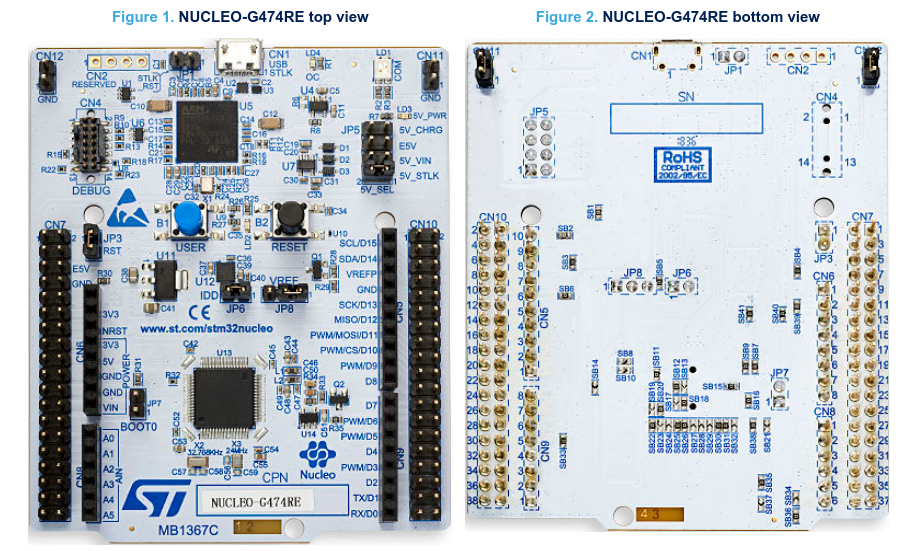
\includegraphics[width=0.8\linewidth]{stm32g474.png}
    \caption{Microcontrolador STM32G474RE empleado en el desarrollo del sistema}
    \label{fig:stm32g474}
\end{figure}

\subsubsection{Resistencias}

Durante el desarrollo del prototipo fue necesario incorporar una serie de resistencias externas, ya que este tipo de componentes pasivos no pueden implementarse mediante los periféricos internos del microcontrolador. Para ello se emplearon resistencias SMD debido a su disponibilidad en el laboratorio, su reducido tamaño y su facilidad de integración en montajes experimentales.

Estas resistencias forman parte del acondicionamiento analógico externo del sistema y permiten adaptar la etapa de señal utilizada durante las pruebas experimentales.

\subsubsection{Software}

\begin{figure}[H]
    \centering
    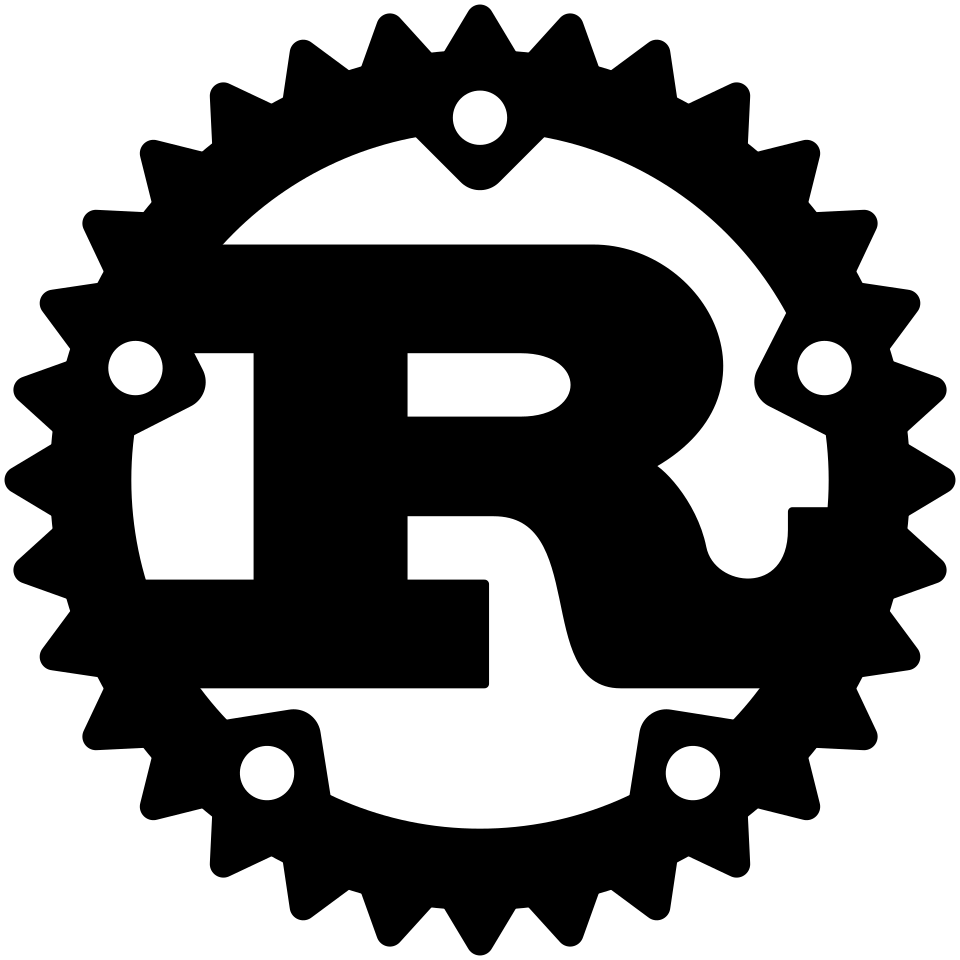
\includegraphics[width=0.22\textwidth]{rust-logo.png}
    \caption{Logotipo del lenguaje Rust.}
    \label{fig:rust-logo}
\end{figure}

El desarrollo del proyecto se ha llevado a cabo utilizando herramientas orientadas al software embebido moderno, destacando el uso del lenguaje \textbf{Rust} para la programación del microcontrolador STM32G474RE. En lugar de utilizar \textit{STM32CubeIDE}, empleado habitualmente en los proyectos académicos sobre microcontroladores STM32, se optó por un entorno más flexible basado en editores de texto y herramientas específicas de Rust. 

Los entornos de desarrollo utilizados fueron:

\begin{itemize}
    \item \textbf{Rust}: lenguaje principal del firmware.
    \item \textbf{Cargo}: compilación y gestión de dependencias.
    \item \textbf{probe-rs}: carga y depuración sobre la placa.
    \item \textbf{defmt}: trazas compactas para sistemas embebidos.
    \item \textbf{Texmaker y LaTeX}: redacción de la memoria.
    \item \textbf{WaveForms}: validación experimental con Analog Discovery 3.
\end{itemize}

\myparagraph{Ventajas del uso de Rust en sistemas embebidos}

El empleo de Rust en el desarrollo del firmware ofrece una serie de beneficios significativos, destacando la \textbf{seguridad de memoria garantizada} en tiempo de compilación y su modelo de propiedad \cite{rustbook}. Además, para la implementación específica en sistemas embebidos, se han seguido las prácticas de gestión de periféricos documentadas en la literatura especializada \cite{matthes2023}.

\begin{itemize}
    \item Seguridad de memoria en un entorno sin sistema operativo.
    \item Control de bajo nivel mediante acceso a registros sin renunciar a comprobaciones del compilador.
    \item Ecosistema de depuración moderno mediante \texttt{probe-rs} y \texttt{defmt}.
\end{itemize}

\myparagraph{Desventajas y desafíos del uso de Rust}

A pesar de sus ventajas, el uso de Rust en entornos embebidos presenta algunas limitaciones:

\begin{itemize}
    \item \textbf{Ecosistema menos maduro que C/C++}, especialmente en cuanto a HALs específicos para cada microcontrolador.
    \item \textbf{Curva de aprendizaje más pronunciada} debido al sistema de propiedad y préstamo del lenguaje.
    \item \textbf{Documentación menos extensa} en comparación con marcos tradicionales como STM32Cube.
    \item Necesidad de una \textbf{configuración inicial más manual}, incluyendo \texttt{linker scripts}, soporte \texttt{no\_std}, configuración del arranque y selección del runtime.
    \item Limitaciones en el uso de librerías externas escritas en C, que requieren interfaces \texttt{unsafe}.
\end{itemize}

En conjunto, Rust representa una alternativa moderna, segura y de alto rendimiento para el desarrollo embebido, y su empleo en este proyecto contribuye a explorar prácticas actuales y futuras tendencias en la industria.

\subsubsection{Infraestructura de compilación y ejecución}

Aunque el objetivo principal del proyecto es la generación y adquisición de señales analógicas, una parte esencial del desarrollo consistió en preparar una infraestructura de ejecución \textit{bare-metal} en Rust. A diferencia de una aplicación convencional ejecutada sobre un sistema operativo, el firmware desarrollado se ejecuta directamente sobre el microcontrolador, sin biblioteca estándar, sin sistema de ficheros y sin servicios proporcionados por un sistema operativo.

Esto implica que el proyecto debe definir explícitamente cómo se compila el código para una arquitectura distinta a la del ordenador de desarrollo, cómo se enlaza el binario resultante en la memoria del microcontrolador, cómo se carga el programa en la placa y cómo se obtiene información de depuración durante la ejecución.

\myparagraph{Configuración del paquete con \texttt{Cargo.toml}}

El archivo \texttt{Cargo.toml} actúa como descriptor principal del proyecto Rust. En él se definen el nombre del paquete, la edición del lenguaje utilizada, los binarios disponibles, las dependencias externas y los perfiles de compilación.

En este proyecto se emplean dependencias específicas para sistemas embebidos, entre las que destacan:

\begin{itemize}
    \item \texttt{cortex-m}: proporciona acceso a funcionalidades comunes del núcleo ARM Cortex-M.
    \item \texttt{cortex-m-rt}: incluye el entorno mínimo de arranque necesario para ejecutar código Rust en microcontroladores Cortex-M.
    \item \texttt{stm32g4}: proporciona acceso a los registros específicos de la familia STM32G4 mediante una capa PAC (\textit{Peripheral Access Crate}).
    \item \texttt{defmt} y \texttt{defmt-rtt}: permiten generar trazas de depuración compactas y eficientes.
    \item \texttt{panic-probe}: define el comportamiento del sistema ante errores críticos o situaciones de pánico.
\end{itemize}

Durante el desarrollo se trabajó con pruebas independientes para validar progresivamente partes concretas del sistema, como la lectura del ADC, la generación mediante DAC o el funcionamiento de pines GPIO, antes de integrarlas en el firmware principal. En la versión final documentada, estas funcionalidades quedan concentradas en el binario principal \texttt{main.rs}.

\myparagraph{Compilación cruzada con \texttt{.cargo/config.toml}}

El archivo \texttt{.cargo/config.toml} define la configuración específica de compilación para el microcontrolador. En un ordenador convencional, Rust compila por defecto para la arquitectura de la propia máquina. Sin embargo, en este proyecto el programa debe ejecutarse sobre un ARM Cortex-M4F, por lo que es necesario realizar compilación cruzada.

Para ello se selecciona el target:

\begin{center}
\texttt{thumbv7em-none-eabihf}
\end{center}

Este target corresponde a microcontroladores ARM Cortex-M4 y Cortex-M7 con unidad de coma flotante hardware. La parte \texttt{none} indica que no existe sistema operativo, y por tanto el programa debe construirse como firmware autónomo.

El mismo archivo configura también el \textit{runner} empleado por Cargo. Gracias a esta configuración, el comando:

\begin{center}
\texttt{cargo run --release --bin main}
\end{center}

no solo compila el firmware, sino que además invoca \texttt{probe-rs} para cargarlo directamente en la placa STM32G474RE. Esto simplifica el ciclo de desarrollo, ya que permite compilar, flashear y ejecutar desde una única orden.

También se especifican opciones de enlazado, como el uso de \texttt{flip-link} y de los scripts \texttt{link.x} y \texttt{defmt.x}. Estos elementos son necesarios para situar correctamente el programa en memoria y para habilitar el sistema de trazas usado por \texttt{defmt}.

\myparagraph{Mapa de memoria con \texttt{memory.x}}



% ============================================================
% DIAGRAMA 3: DISTRIBUCIÓN CONCEPTUAL FLASH / RAM
% ============================================================

\begin{figure}[H]
\centering
\resizebox{0.85\textwidth}{!}{%
\begin{tikzpicture}[
    mem/.style={
        rectangle,
        draw,
        rounded corners,
        minimum width=4.2cm,
        minimum height=6.3cm,
        align=center,
        font=\small
    },
    item/.style={
        rectangle,
        draw,
        rounded corners,
        minimum width=3.5cm,
        minimum height=0.75cm,
        align=center,
        font=\small
    },
    arrow/.style={-{Latex[length=2.8mm]}, thick}
]

% Bloques de memoria
\node[mem] (flash) at (0,0) {};
\node[font=\bfseries] at (0,2.65) {FLASH};

\node[item] (code) at (0,1.65) {Código ejecutable};
\node[item] (sine) at (0,0.55) {\texttt{TABLA\_SENO}};
\node[item] (profiles) at (0,-0.55) {\texttt{PERFILES}};
\node[item] (constants) at (0,-1.65) {Constantes del firmware};

\node[mem] (ram) at (6,0) {};
\node[font=\bfseries] at (6,2.65) {RAM};

\node[item] (buffer) at (6,1.65) {\texttt{adc\_buffer}};
\node[item] (profileactual) at (6,0.55) {\texttt{perfil\_actual}};
\node[item] (stack) at (6,-0.55) {Pila};
\node[item] (temp) at (6,-1.65) {Variables temporales};

% Flechas conceptuales
\draw[arrow] (sine.east) -- node[above, font=\scriptsize]{lectura por DMA} (buffer.west);
\draw[arrow] (profiles.east) -- node[below, font=\scriptsize]{selección de perfil} (profileactual.west);

% Nota inferior
\node[
    draw,
    rounded corners,
    align=center,
    font=\small,
    text width=9.7cm
] at (3,-3.7) {
    Los datos constantes se almacenan en Flash, mientras que los datos modificables durante la ejecución se ubican en RAM.
};

\end{tikzpicture}%
}
\caption{Distribución conceptual de los elementos principales del firmware entre memoria Flash y RAM.}
\label{fig:memoria-flash-ram}
\end{figure}

\subsubsection{Ejecución del firmware y organización de memoria}

\begin{figure}[H]
    \centering
    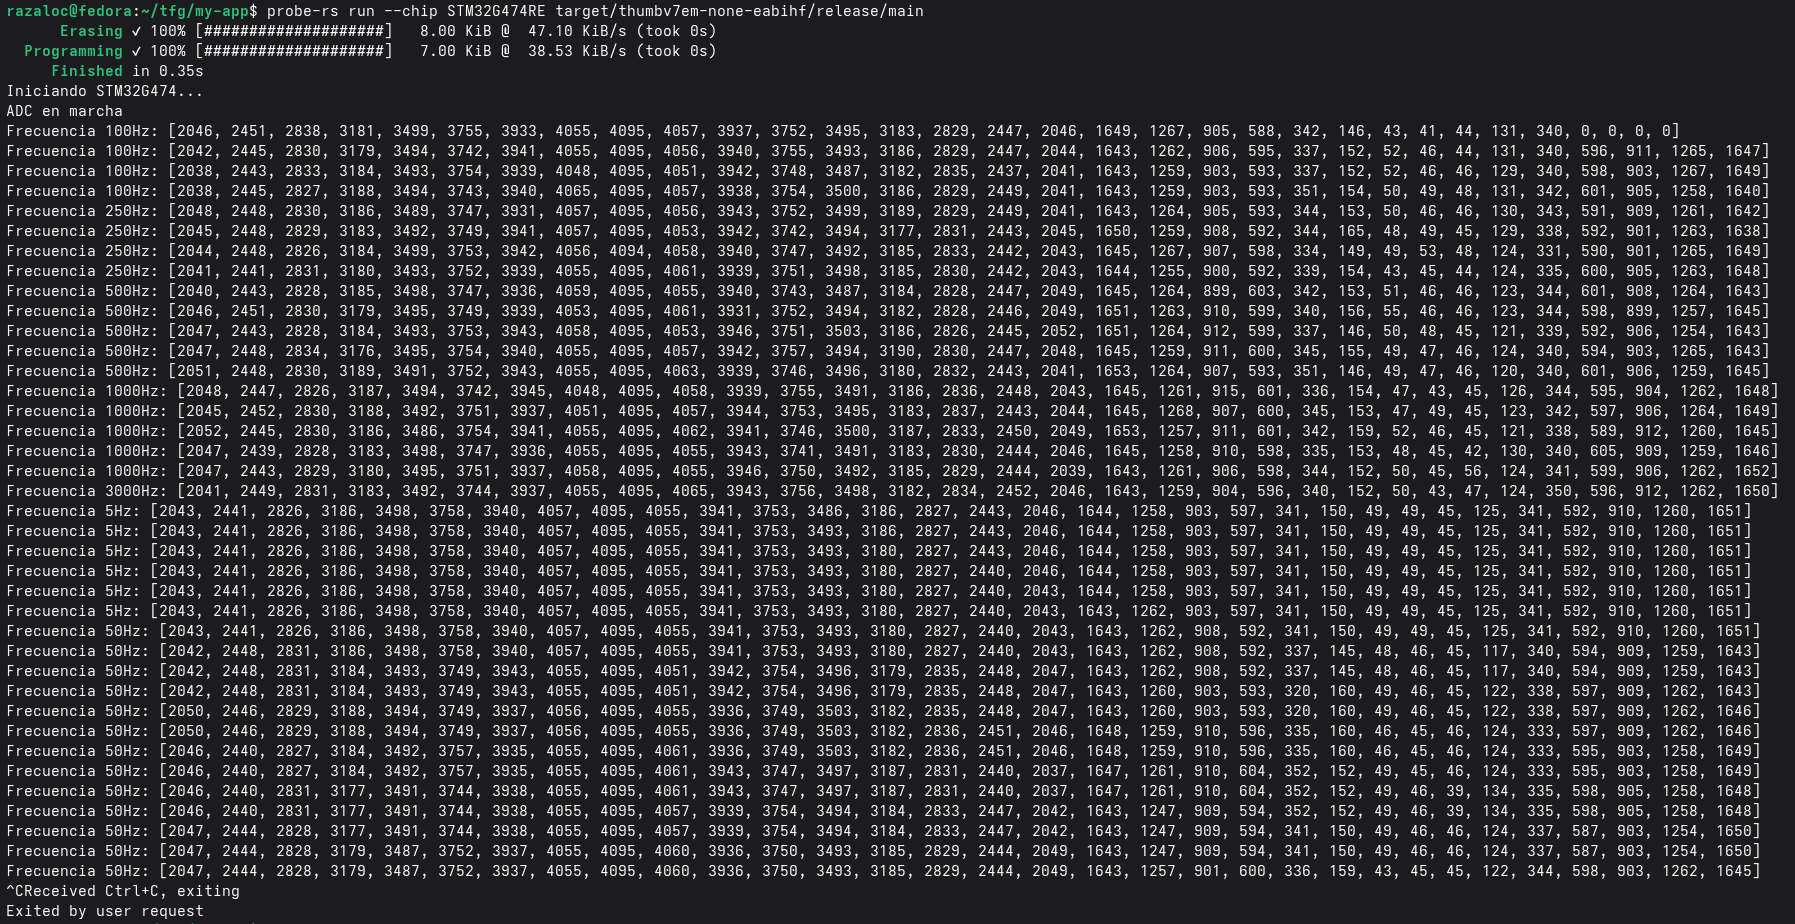
\includegraphics[width=0.85\textwidth]{ejecucion-firmware.png}
    \caption{Salida por consola durante la ejecución del firmware, mostrando la frecuencia activa y las muestras adquiridas por el ADC.}
    \label{fig:ejecucion-firmware}
\end{figure}

El archivo \texttt{memory.x} define las regiones de memoria disponibles para el firmware. En un sistema embebido, el enlazador necesita conocer la dirección de inicio y el tamaño de la memoria Flash y de la memoria RAM del microcontrolador.

La memoria Flash se utiliza principalmente para almacenar el código del programa y las constantes, mientras que la RAM contiene variables globales modificables, pila, buffers y datos temporales de ejecución. En este proyecto, el buffer utilizado por el DMA para almacenar muestras del ADC depende directamente de esta configuración de memoria.

Además de los buffers utilizados por DMA, el firmware emplea memoria no volátil para almacenar tablas constantes de funcionamiento. La tabla senoidal y los perfiles de frecuencia se declaran como constantes, por lo que el compilador los ubica en la región de memoria Flash. Esto permite disponer de varias configuraciones predefinidas sin ocupar RAM dinámica ni requerir asignación en tiempo de ejecución, algo especialmente adecuado en un entorno \textit{bare-metal} y \texttt{no\_std}.

Un ejemplo simplificado de este archivo es:

\begin{lstlisting}
MEMORY
{
  FLASH : ORIGIN = 0x08000000, LENGTH = 512K
  RAM   : ORIGIN = 0x20000000, LENGTH = 96K
}
\end{lstlisting}

En este proyecto, la memoria Flash contiene tanto el código ejecutable como los datos constantes del sistema, entre ellos la tabla de muestras de la señal senoidal y la tabla de perfiles de frecuencia. Por otro lado, la RAM se reserva para elementos modificables durante la ejecución, como el índice del perfil activo y el búfer circular utilizado por el DMA para almacenar las muestras procedentes del ADC.

Esta configuración debe coincidir con las características reales del microcontrolador utilizado. Una definición incorrecta del mapa de memoria puede provocar errores de enlazado, desaprovechamiento de memoria disponible o fallos en tiempo de ejecución si el programa accede a regiones no válidas.



\myparagraph{Código común de arranque y errores en \texttt{src/lib.rs}}

El archivo \texttt{src/lib.rs} contiene parte de la infraestructura común utilizada por los distintos binarios del proyecto. En él se integran elementos como el sistema de logging global, el comportamiento ante pánicos y el tratamiento básico de excepciones.

En aplicaciones Rust convencionales, la biblioteca estándar proporciona mecanismos de gestión de errores, impresión por consola y finalización del programa. En un sistema \textit{no\_std}, estas funcionalidades no existen por defecto, por lo que deben definirse explícitamente.

En este proyecto se emplea \texttt{panic-probe} junto con \texttt{defmt} para poder observar errores durante la ejecución mediante la sonda de depuración. Esto facilita detectar fallos en fases tempranas del desarrollo, especialmente cuando el programa se ejecuta sin pantalla, teclado ni sistema operativo.

\myparagraph{Estructura de binarios de prueba}

Durante el desarrollo se emplearon pruebas independientes para validar cada periférico por separado antes de realizar la integración completa. Esta estrategia permitió reducir el riesgo técnico antes de concentrar la funcionalidad en el firmware principal.

Por ejemplo, se desarrollaron pruebas específicas para:

\begin{itemize}
    \item Comprobar el entorno mínimo de ejecución y depuración.
    \item Configurar un pin GPIO como salida.
    \item Validar la lectura del ADC en el pin PA0.
    \item Generar una tensión analógica mediante el DAC en PA4.
    \item Integrar generación y adquisición en un mismo flujo.
\end{itemize}

Esta organización redujo la complejidad durante la depuración. En lugar de probar directamente todo el sistema completo, cada bloque funcional se verificó de forma incremental. Posteriormente, las partes validadas se integraron en el binario principal \texttt{main.rs}.

\myparagraph{Depuración con \texttt{defmt} y \texttt{probe-rs}}

La depuración de firmware embebido presenta dificultades adicionales respecto al software convencional, ya que no existe una salida estándar por consola. Para resolver este problema se utilizó \texttt{defmt}, un sistema de logging diseñado específicamente para microcontroladores.

Las trazas generadas por el firmware se transmiten mediante RTT y son recogidas en el ordenador de desarrollo a través de \texttt{probe-rs}. Esto permite observar mensajes de estado, valores leídos del ADC, avisos de desviación y eventos relevantes del sistema sin necesidad de implementar inicialmente una comunicación UART propia.

Este mecanismo resultó especialmente útil durante la fase de pruebas, ya que permitió comprobar si los periféricos estaban siendo inicializados correctamente y si el buffer de muestras del ADC recibía datos durante la ejecución.

\myparagraph{Importancia de la infraestructura en el proyecto}

La infraestructura descrita no constituye un elemento auxiliar, sino una parte fundamental del proyecto. Sin ella, el código Rust no podría ejecutarse correctamente sobre el STM32G474RE. La configuración de compilación cruzada, el mapa de memoria, el sistema de arranque, los perfiles de optimización, la carga mediante \texttt{probe-rs} y la depuración mediante \texttt{defmt} forman la base sobre la que se construye el firmware de generación y adquisición de señal.

Por tanto, el desarrollo del sistema no se limitó únicamente a programar los periféricos ADC, DAC, DMA y TIM6, sino que también incluyó la creación de un entorno completo de desarrollo embebido en Rust, reproducible y adaptado a la placa utilizada.

\subsubsection{Instrumentación de laboratorio}

Para la validación del sistema y el análisis de las señales generadas y adquiridas, se empleó una \textbf{Analog Discovery 3} de Digilent proporcionada por el departamento. Este equipo permitió observar en tiempo real tanto la señal senoidal generada por el convertidor digital--analógico (DAC) como la señal capturada mediante el convertidor analógico--digital (ADC), facilitando la verificación del correcto funcionamiento del sistema.

Durante el desarrollo se utilizaron las entradas analógicas del equipo y el software WaveForms para visualizar y exportar las señales medidas. La instrumentación se empleó principalmente en las fases de prueba del generador de señal, calibración del sistema de adquisición y verificación del comportamiento bajo carga conocida.

El uso de este instrumento resultó fundamental para comprobar la integridad de la forma de onda generada, detectar posibles distorsiones o errores de sincronización y contrastar experimentalmente las muestras observadas mediante las trazas del firmware.



\subsubsection{Otros componentes considerados}
Durante la fase de diseño, se evaluó la posibilidad de utilizar integrados externos para la conversión de señal (DAC/ADC de mayor resolución). Sin embargo, tras analizar las especificaciones del \textbf{STM32G474RE}, se determinó que sus convertidores internos de 12 bits y su alta velocidad de muestreo eran más que suficientes para aplicaciones biomédicas de este rango, cumpliendo así con el requisito \textbf{R1} de maximizar la integración.

\subsection{Análisis de costes estimados}

El desarrollo del presente proyecto implica distintos tipos de costes que van más allá del material estrictamente utilizado. Para ofrecer una visión más realista del esfuerzo necesario en un contexto profesional, se distinguen dos categorías principales: costes de materiales y costes derivados del trabajo de ingeniería. Las cifras presentadas constituyen estimaciones orientativas con fines académicos.

\subsubsection*{Costes de materiales}

\begin{table}[H]
    \centering
    \begin{tabular}{|l|r|}
        \hline
        \textbf{Componente} & \textbf{Coste estimado} \\ \hline
        Tarjeta Nucleo-G474RE & 25.00 € \\ \hline
        Componentes pasivos y placa perforada & 5.00 € \\ \hline
        Cableado, conectores y consumibles de laboratorio & 15.00 € \\ \hline
        Software (Rust, LaTeX, WaveForms y herramientas Open Source) & 0.00 € \\ \hline
        \textbf{Subtotal materiales} & \textbf{45.00 €} \\ \hline
    \end{tabular}
    \caption{Costes asociados a materiales utilizados en el proyecto}
\end{table}

\subsubsection*{Equipamiento de laboratorio}

La instrumentación utilizada durante las pruebas, en concreto la \textbf{Analog Discovery 3} de Digilent, fue proporcionada por el departamento. Por tanto, no supuso un coste de adquisición para el proyecto y no se incluye dentro del presupuesto estimado.

\subsubsection*{Costes de ingeniería}

El desarrollo del firmware, diseño electrónico, pruebas experimentales, documentación y elaboración de la memoria implicaron una dedicación estimada de 310 horas de trabajo técnico, coherente con la planificación de hitos descrita posteriormente. Para efectos comparativos con un entorno profesional, se considera una tarifa de 30 € por hora.

\begin{table}[H]
    \centering
    \begin{tabular}{|l|r|}
        \hline
        \textbf{Concepto} & \textbf{Coste estimado} \\ \hline
        Trabajo de ingeniería (310 h $\times$ 30 €/h) & 9300.00 € \\ \hline
        \textbf{Subtotal ingeniería} & \textbf{9300.00 €} \\ \hline
    \end{tabular}
    \caption{Estimación del coste de desarrollo técnico}
\end{table}


\bigskip

Considerando el conjunto de categorías anteriores, el coste total estimado del proyecto asciende a:

\begin{center}
\textbf{Coste total estimado: 9345.00 €}
\end{center}


\subsection{Planificación de hitos}

El proyecto se ha dividido en cinco hitos principales. La planificación parte del día \textbf{2 de marzo de 2026} y finaliza el día \textbf{26 de mayo de 2026}. Se organiza considerando jornadas de trabajo de aproximadamente \textbf{5 horas}, con una dedicación total estimada de \textbf{310 horas}.

La distribución temporal se ha organizado de forma secuencial: primero se reserva un bloque amplio para el aprendizaje de Rust embebido y la configuración del entorno, posteriormente se desarrolla la generación de señal mediante DAC, después la adquisición mediante ADC, y finalmente se realizan las pruebas experimentales con la Analog Discovery 3 antes de la redacción final de la memoria.

\subsubsection{H1 -- Aprendizaje y entorno Rust embebido funcional}

\begin{table}[H]
\centering
\small
\begin{tabularx}{\textwidth}{lXccr}
\toprule
\textbf{Código} & \textbf{Tarea} & \textbf{Inicio} & \textbf{Fin} & \textbf{Horas} \\
\midrule
T1.1 & Estudio inicial de Rust & 02/03/2026 & 04/03/2026 & 15 \\
T1.2 & Rust embebido: \textit{no\_std} y \textit{bare-metal} & 05/03/2026 & 09/03/2026 & 15 \\
T1.3 & Ecosistema: \texttt{cortex-m}, PAC, \texttt{defmt} y \texttt{probe-rs} & 10/03/2026 & 12/03/2026 & 15 \\
T1.4 & Instalación y configuración de herramientas & 13/03/2026 & 16/03/2026 & 10 \\
T1.5 & Estructura del proyecto y \texttt{Cargo.toml} & 17/03/2026 & 18/03/2026 & 10 \\
T1.6 & Mapa de memoria y enlazado & 19/03/2026 & 20/03/2026 & 10 \\
T1.7 & Primer firmware mínimo & 23/03/2026 & 23/03/2026 & 5 \\
T1.8 & Depuración con \texttt{defmt} y \texttt{probe-rs} & 24/03/2026 & 24/03/2026 & 5 \\
\midrule
\multicolumn{4}{r}{\textbf{Subtotal H1}} & \textbf{85} \\
\bottomrule
\end{tabularx}
\caption{Planificación del hito H1}
\label{tab:hito1}
\end{table}

\subsubsection{H2 -- Generación de señal senoidal mediante DAC}

\begin{table}[H]
\centering
\small
\begin{tabularx}{\textwidth}{lXccr}
\toprule
\textbf{Código} & \textbf{Tarea} & \textbf{Inicio} & \textbf{Fin} & \textbf{Horas} \\
\midrule
T2.1 & Estudio de DAC, TIM6, DMA y DMAMUX & 25/03/2026 & 26/03/2026 & 10 \\
T2.2 & Configuración de relojes y GPIOA & 27/03/2026 & 27/03/2026 & 5 \\
T2.3 & Tabla senoidal de 32 muestras & 30/03/2026 & 31/03/2026 & 10 \\
T2.4 & Configuración de TIM6 como TRGO & 01/04/2026 & 02/04/2026 & 10 \\
T2.5 & Configuración del DAC & 03/04/2026 & 07/04/2026 & 15 \\
T2.6 & DMA circular hacia DAC & 08/04/2026 & 09/04/2026 & 10 \\
T2.7 & Perfiles de frecuencia & 10/04/2026 & 10/04/2026 & 5 \\
T2.8 & Pruebas preliminares mediante \texttt{defmt} & 13/04/2026 & 13/04/2026 & 5 \\
\midrule
\multicolumn{4}{r}{\textbf{Subtotal H2}} & \textbf{70} \\
\bottomrule
\end{tabularx}
\caption{Planificación del hito H2}
\label{tab:hito2}
\end{table}

\subsubsection{H3 -- Adquisición de señal mediante ADC}

\begin{table}[H]
\centering
\small
\begin{tabularx}{\textwidth}{lXccr}
\toprule
\textbf{Código} & \textbf{Tarea} & \textbf{Inicio} & \textbf{Fin} & \textbf{Horas} \\
\midrule
T3.1 & Estudio del ADC y calibración & 14/04/2026 & 15/04/2026 & 10 \\
T3.2 & Configuración de PA0 y canal ADC & 16/04/2026 & 16/04/2026 & 5 \\
T3.3 & Reloj, regulador y calibración del ADC & 17/04/2026 & 20/04/2026 & 10 \\
T3.4 & Disparo externo mediante TIM6 & 21/04/2026 & 22/04/2026 & 10 \\
T3.5 & DMA circular para búfer ADC & 23/04/2026 & 24/04/2026 & 10 \\
T3.6 & Integración DAC-ADC-TIM6-DMA & 27/04/2026 & 28/04/2026 & 10 \\
T3.7 & Lectura del búfer y trazas \texttt{defmt} & 29/04/2026 & 29/04/2026 & 5 \\
\midrule
\multicolumn{4}{r}{\textbf{Subtotal H3}} & \textbf{60} \\
\bottomrule
\end{tabularx}
\caption{Planificación del hito H3}
\label{tab:hito3}
\end{table}

\subsubsection{H4 -- Validación experimental con Analog Discovery 3}

\begin{table}[H]
\centering
\small
\begin{tabularx}{\textwidth}{lXccr}
\toprule
\textbf{Código} & \textbf{Tarea} & \textbf{Inicio} & \textbf{Fin} & \textbf{Horas} \\
\midrule
T4.1 & Preparación del entorno de pruebas & 30/04/2026 & 30/04/2026 & 5 \\
T4.2 & Plan de pruebas experimentales & 01/05/2026 & 01/05/2026 & 5 \\
T4.3 & Medida de señal DAC con Analog Discovery 3 & 04/05/2026 & 05/05/2026 & 10 \\
T4.4 & Pruebas con cargas conocidas & 06/05/2026 & 07/05/2026 & 10 \\
T4.5 & Prueba de estabilidad & 08/05/2026 & 08/05/2026 & 5 \\
T4.6 & Análisis y capturas de resultados & 11/05/2026 & 12/05/2026 & 10 \\
\midrule
\multicolumn{4}{r}{\textbf{Subtotal H4}} & \textbf{45} \\
\bottomrule
\end{tabularx}
\caption{Planificación del hito H4}
\label{tab:hito4}
\end{table}

\subsubsection{H5 -- Documentación y cierre del proyecto}

\begin{table}[H]
\centering
\small
\begin{tabularx}{\textwidth}{lXccr}
\toprule
\textbf{Código} & \textbf{Tarea} & \textbf{Inicio} & \textbf{Fin} & \textbf{Horas} \\
\midrule
T5.1 & Estructura final, resumen e índice & 13/05/2026 & 13/05/2026 & 5 \\
T5.2 & Introducción, objetivos y descripción & 14/05/2026 & 14/05/2026 & 5 \\
T5.3 & Estado del arte y fundamentos & 15/05/2026 & 18/05/2026 & 10 \\
T5.4 & Planificación, requisitos y costes & 19/05/2026 & 20/05/2026 & 10 \\
T5.5 & Desarrollo técnico y firmware & 21/05/2026 & 21/05/2026 & 5 \\
T5.6 & Pruebas, resultados y conclusiones & 22/05/2026 & 22/05/2026 & 5 \\
T5.7 & Bibliografía, anexos y revisión final & 25/05/2026 & 26/05/2026 & 10 \\
\midrule
\multicolumn{4}{r}{\textbf{Subtotal H5}} & \textbf{50} \\
\bottomrule
\end{tabularx}
\caption{Planificación del hito H5}
\label{tab:hito5}
\end{table}

\subsubsection{Resumen temporal}

\begin{table}[H]
\centering
\small
\begin{tabular}{lccr}
\toprule
\textbf{Hito} & \textbf{Inicio} & \textbf{Fin} & \textbf{Horas} \\
\midrule
H1 -- Aprendizaje y entorno Rust embebido & 02/03/2026 & 24/03/2026 & 85 \\
H2 -- Generación de señal mediante DAC & 25/03/2026 & 13/04/2026 & 70 \\
H3 -- Adquisición de señal mediante ADC & 14/04/2026 & 29/04/2026 & 60 \\
H4 -- Validación experimental con Analog Discovery 3 & 30/04/2026 & 12/05/2026 & 45 \\
H5 -- Documentación y cierre del proyecto & 13/05/2026 & 26/05/2026 & 50 \\
\midrule
\textbf{Total} & 02/03/2026 & 26/05/2026 & \textbf{310} \\
\bottomrule
\end{tabular}
\caption{Resumen de la planificación temporal del proyecto}
\label{tab:resumen_planificacion}
\end{table}

\clearpage
\newgeometry{
    left=0.5cm,
    right=0.5cm,
    top=0.7cm,
    bottom=0.7cm
}

\begin{landscape}
\subsubsection{Diagrama de Gantt}

En la Figura~\ref{fig:gantt_hitos} se representa la planificación temporal del proyecto dividida por hitos. El calendario comienza el 2 de marzo de 2026 y finaliza el 26 de mayo de 2026, con una dedicación total estimada de 310 horas.

\begin{figure}[H]
\centering
\tiny

\begin{ganttchart}[
    hgrid,
    vgrid,
    time slot format=isodate,
    x unit=0.22cm,
    y unit chart=0.30cm,
    bar height=0.25,
    group height=0.25,
    milestone height=0.30,
    title height=0.65,
    title label font=\tiny,
    bar label font=\tiny,
    group label font=\tiny\bfseries,
    milestone label font=\tiny\itshape,
    bar label node/.append style={text width=0.8cm, align=right},
    group label node/.append style={text width=2.0cm, align=right},
    bar/.append style={fill=gray!35},
    group/.append style={fill=gray!60},
    milestone/.append style={fill=black}
]{2026-03-02}{2026-05-26}

\gantttitlecalendar{month=name, week} \\
% ===================== H1 =====================
\ganttgroup{H1 -- Rust}{2026-03-02}{2026-03-24} \\
\ganttbar{T1.1}{2026-03-02}{2026-03-04} \\
\ganttbar{T1.2}{2026-03-05}{2026-03-09} \\
\ganttbar{T1.3}{2026-03-10}{2026-03-12} \\
\ganttbar{T1.4}{2026-03-13}{2026-03-16} \\
\ganttbar{T1.5}{2026-03-17}{2026-03-18} \\
\ganttbar{T1.6}{2026-03-19}{2026-03-20} \\
\ganttbar{T1.7}{2026-03-23}{2026-03-23} \\
\ganttbar{T1.8}{2026-03-24}{2026-03-24} \\
\ganttmilestone{H1}{2026-03-24} \\

% ===================== H2 =====================
\ganttgroup{H2 -- DAC}{2026-03-25}{2026-04-13} \\
\ganttbar{T2.1}{2026-03-25}{2026-03-26} \\
\ganttbar{T2.2}{2026-03-27}{2026-03-27} \\
\ganttbar{T2.3}{2026-03-30}{2026-03-31} \\
\ganttbar{T2.4}{2026-04-01}{2026-04-02} \\
\ganttbar{T2.5}{2026-04-03}{2026-04-07} \\
\ganttbar{T2.6}{2026-04-08}{2026-04-09} \\
\ganttbar{T2.7}{2026-04-10}{2026-04-10} \\
\ganttbar{T2.8}{2026-04-13}{2026-04-13} \\
\ganttmilestone{H2}{2026-04-13} \\

% ===================== H3 =====================
\ganttgroup{H3 -- ADC}{2026-04-14}{2026-04-29} \\
\ganttbar{T3.1}{2026-04-14}{2026-04-15} \\
\ganttbar{T3.2}{2026-04-16}{2026-04-16} \\
\ganttbar{T3.3}{2026-04-17}{2026-04-20} \\
\ganttbar{T3.4}{2026-04-21}{2026-04-22} \\
\ganttbar{T3.5}{2026-04-23}{2026-04-24} \\
\ganttbar{T3.6}{2026-04-27}{2026-04-28} \\
\ganttbar{T3.7}{2026-04-29}{2026-04-29} \\
\ganttmilestone{H3}{2026-04-29} \\

% ===================== H4 =====================
\ganttgroup{H4 -- Pruebas}{2026-04-30}{2026-05-12} \\
\ganttbar{T4.1}{2026-04-30}{2026-04-30} \\
\ganttbar{T4.2}{2026-05-01}{2026-05-01} \\
\ganttbar{T4.3}{2026-05-04}{2026-05-05} \\
\ganttbar{T4.4}{2026-05-06}{2026-05-07} \\
\ganttbar{T4.5}{2026-05-08}{2026-05-08} \\
\ganttbar{T4.6}{2026-05-11}{2026-05-12} \\
\ganttmilestone{H4}{2026-05-12} \\

% ===================== H5 =====================
\ganttgroup{H5 -- Doc.}{2026-05-13}{2026-05-26} \\
\ganttbar{T5.1}{2026-05-13}{2026-05-13} \\
\ganttbar{T5.2}{2026-05-14}{2026-05-14} \\
\ganttbar{T5.3}{2026-05-15}{2026-05-18} \\
\ganttbar{T5.4}{2026-05-19}{2026-05-20} \\
\ganttbar{T5.5}{2026-05-21}{2026-05-21} \\
\ganttbar{T5.6}{2026-05-22}{2026-05-22} \\
\ganttbar{T5.7}{2026-05-25}{2026-05-26} \\
\ganttmilestone{Entrega}{2026-05-26}

\end{ganttchart}

\caption{Diagrama de Gantt del proyecto dividido por hitos}
\label{fig:gantt_hitos}
\end{figure}

\end{landscape}
\restoregeometry
\clearpage

\section{Desarrollo del proyecto}

\subsection{Fundamentos del Sistema Microcontrolador}
El sistema se apoya en una arquitectura de 32 bits. La clave del rendimiento reside en la interconexión de periféricos mediante el bus \textbf{AHB}, permitiendo que el DMA mueva datos entre el DAC/ADC y la memoria RAM sin intervención del núcleo ARM Cortex-M4, liberando a este para tareas de procesamiento de datos.

\subsection{Diseño del sistema}

% ============================================================
% DIAGRAMA 1: ARQUITECTURA GENERAL DEL SISTEMA
% ============================================================

\begin{figure}[H]
\centering
\resizebox{\textwidth}{!}{%
\begin{tikzpicture}[
    block/.style={
        rectangle,
        draw,
        rounded corners,
        align=center,
        minimum width=3.1cm,
        minimum height=1.15cm,
        font=\small
    },
    smallblock/.style={
        rectangle,
        draw,
        rounded corners,
        align=center,
        minimum width=2.5cm,
        minimum height=0.95cm,
        font=\small
    },
    arrow/.style={
        -{Latex[length=3mm]},
        thick
    },
    dashedarrow/.style={
        -{Latex[length=3mm]},
        thick,
        dashed
    }
]

% Nodos principales
\node[block] (flash) {Memoria Flash\\\texttt{TABLA\_SENO}\\\texttt{PERFILES}};
\node[block, right=2.0cm of flash] (dma_dac) {DMA\\canal DAC};
\node[block, right=2.0cm of dma_dac] (dac) {DAC1\\PA4\\Salida analógica};
\node[block, right=2.0cm of dac] (signal) {Señal senoidal\\generada};

\node[block, below=3cm of signal] (adc) {ADC1\\PA0\\Entrada analógica};
\node[block, left=2.0cm of adc] (dma_adc) {DMA\\canal ADC};
\node[block, left=2.0cm of dma_adc] (ram) {Memoria RAM\\\texttt{adc\_buffer}\\\texttt{perfil\_actual}};

\node[smallblock, below=1.4cm of dma_dac] (tim6) {TIM6\\TRGO};
\node[smallblock, below=1.4cm of flash] (button) {Pulsador\\PC13};

% Flechas de datos
\draw[arrow] (flash) -- node[above, font=\scriptsize]{muestras} (dma_dac);
\draw[arrow] (dma_dac) -- node[above, font=\scriptsize]{transferencia circular} (dac);
\draw[arrow] (dac) -- (signal);
\draw[arrow] (signal) -- node[right, font=\scriptsize]{medición} (adc);
\draw[arrow] (adc) -- node[above, font=\scriptsize]{muestras ADC} (dma_adc);
\draw[arrow] (dma_adc) -- node[above, font=\scriptsize]{búfer circular} (ram);

% Flechas de sincronización
\draw[dashedarrow] (tim6) -- node[right, font=\scriptsize]{disparo} (dma_dac);
\draw[dashedarrow] (tim6) -- node[right, font=\scriptsize]{trigger} (dac);
\draw[dashedarrow] (tim6) -- node[right, font=\scriptsize]{trigger} (adc);

% Control con botón
\draw[dashedarrow] (button) -- node[left, font=\scriptsize]{cambio de perfil} (flash);
\draw[dashedarrow] (button) -- node[below, font=\scriptsize]{actualiza PSC/ARR} (tim6);

\end{tikzpicture}%
}
\caption{Arquitectura general del sistema implementado, mostrando la generación mediante DAC, la adquisición mediante ADC y la sincronización común mediante TIM6.}
\label{fig:arquitectura-general}
\end{figure}


\subsubsection{Funcionamiento integrado}
La generación se basa en una técnica de síntesis digital directa (DDS) simplificada. Una tabla de 32 valores define un ciclo completo de la onda, y el DAC se actualiza mediante eventos de disparo generados por \texttt{TIM6}. Por tanto, la frecuencia de salida depende del reloj de TIM6 y de los divisores enteros configurados:
\[
f_{out} =
\frac{f_{TIM6}}
{(PSC+1)(ARR+1)N_{muestras}}
\]

El firmware no modifica la configuración global del reloj después del arranque. Las medidas realizadas con el osciloscopio son coherentes con un reloj de TIM6 próximo a \(16~MHz\). Debido a la cuantización introducida por \(PSC\) y \(ARR\), las frecuencias obtenidas no coinciden exactamente con los valores inicialmente utilizados como etiquetas.

El mismo disparo hardware se utiliza para coordinar la adquisición mediante \textbf{ADC1}. En lugar de ejecutar un bucle software que escriba cada muestra en el DAC o lea cada conversión del ADC, el firmware configura los periféricos para que TIM6 marque el ritmo y DMA realice las transferencias de datos. La CPU queda reservada principalmente para la inicialización, la selección de perfiles de frecuencia y la monitorización de las muestras adquiridas.

Los perfiles de frecuencia modifican los valores \texttt{PSC} y \texttt{ARR} de TIM6, permitiendo cambiar la frecuencia de generación y adquisición sin alterar la tabla senoidal ni recompilar el programa.


\subsection{Desarrollo del sistema (Fases)}

Las fases F1--F8 describen la evolución técnica seguida durante la implementación y validación del sistema. No sustituyen a los hitos temporales H1--H5 de la planificación, sino que los detallan desde el punto de vista del trabajo realizado: aprendizaje e infraestructura, prototipos de periféricos, integración, selección de perfiles y validación experimental.

\subsubsection{F1: Planteamiento y estudio inicial}

En esta fase se definió el alcance general del proyecto y se realizó un estudio preliminar de su viabilidad técnica. Se analizaron los objetivos principales del trabajo, los requisitos funcionales del sistema y las restricciones impuestas al diseño, tanto a nivel de implementación embebida como de integración hardware.
También se llevó a cabo una primera evaluación de la familia STM32G4, prestando especial atención a sus capacidades analógicas internas. Este estudio permitió comprobar que el microcontrolador STM32G474RE disponía de periféricos adecuados para el desarrollo del proyecto, como DAC, ADC, temporizadores y DMA. A partir de este análisis se justificó la elección de esta plataforma como base del sistema.


\subsubsection{F2: Aprendizaje de Rust embebido e infraestructura}

Durante esta etapa se adquirieron los conocimientos necesarios para el desarrollo de aplicaciones embebidas en Rust. Se estudió el ecosistema \texttt{embedded-hal}, la organización de los paquetes de soporte para microcontroladores STM32 y las herramientas empleadas para la compilación, carga y depuración del firmware.
Asimismo, se configuró la infraestructura básica de desarrollo, incluyendo el entorno de compilación para arquitecturas ARM Cortex-M, el uso de \texttt{probe-rs} para la programación y depuración del microcontrolador, y la estructura inicial del proyecto en Rust. Esta fase resultó fundamental para establecer una base de trabajo estable sobre la que implementar posteriormente los distintos periféricos.
Dado que el lenguaje C continúa siendo la opción predominante en el ámbito de los sistemas embebidos, se detectó que el ecosistema Rust para la familia STM32G4 presenta todavía ciertas limitaciones. En particular, algunas capas de abstracción hardware disponibles se encuentran en fases tempranas de desarrollo o no ofrecen soporte completo para todos los periféricos requeridos. Por ello, fue necesario trabajar en algunos casos a un nivel más próximo a los registros del microcontrolador.


\subsubsection{F3: Estudio del STM32G474RE y periféricos analógicos}

En esta fase se profundizó en el estudio del microcontrolador STM32G474RE y de los periféricos necesarios para el proyecto: DAC, ADC, DMA y temporizadores. También se estudiaron los registros específicos asociados a cada bloque, ya que el soporte de alto nivel disponible en Rust no cubría completamente todas las funcionalidades necesarias.

Este análisis permitió definir la arquitectura interna del firmware: generación mediante DAC, temporización mediante TIM6, transferencia automática por DMA y adquisición mediante ADC.


\subsubsection{F4: Prototipos mínimos de GPIO, DAC y ADC}

Una vez configurado el entorno de desarrollo y estudiados los periféricos principales, se implementaron prototipos mínimos para validar el funcionamiento básico del microcontrolador. Inicialmente se realizaron pruebas con GPIO, con el objetivo de comprobar la correcta compilación, carga y ejecución del firmware sobre la placa de desarrollo.
Posteriormente, se desarrollaron pruebas independientes para el DAC y el ADC. En el caso del DAC, se verificó la capacidad de generar valores analógicos simples a partir de datos digitales definidos por software. En el caso del ADC, se comprobó la lectura de señales analógicas y se implementó una rutina de calibración inicial para compensar el error de offset interno del chip.
Estos prototipos permitieron validar de forma incremental cada bloque funcional antes de abordar su integración completa. Además, facilitaron la detección temprana de errores de configuración y permitieron familiarizarse con el acceso a los registros del STM32G474RE desde Rust.


\subsubsection{F5: Integración DAC-DMA-TIM6}

En esta fase se integraron el DAC, el controlador DMA y el temporizador TIM6 para implementar la generación automática de señal. Se definió una tabla senoidal en memoria y se configuró el DMA para transferir sus muestras al DAC siguiendo el ritmo marcado por TIM6. Esta etapa permitió pasar de pruebas manuales de salida analógica a una generación periódica y autónoma.


\subsubsection{F6: Integración ADC-DMA y lectura de muestras}

Durante esta etapa se configuró el ADC junto con el DMA para realizar la adquisición automática de muestras analógicas. Se ajustó la calibración inicial, el canal de entrada y el modo de conversión, y se configuró un búfer de muestras en memoria para recibir los resultados. Con ello se cerró el ciclo de generación y adquisición dentro del propio microcontrolador.



\subsubsection{F7: Selección de perfiles de frecuencia mediante pulsador}

Una vez validado el funcionamiento conjunto del DAC, ADC, DMA y TIM6, se incorporó la selección de distintas frecuencias sin recompilar el firmware. Cada perfil almacena los valores de prescaler (\texttt{PSC}) y auto-reload (\texttt{ARR}) de TIM6, y el pulsador de usuario conectado a \texttt{PC13} permite recorrerlos durante la ejecución. Esta ampliación facilita realizar ensayos a distintas frecuencias de excitación manteniendo la sincronización entre generación y adquisición.



% ============================================================
% DIAGRAMA 4: CAMBIO DE PERFIL MEDIANTE PULSADOR
% ============================================================

\begin{figure}[H]
\centering
\resizebox{0.72\textwidth}{!}{%
\begin{tikzpicture}[
    startstop/.style={
        ellipse,
        draw,
        align=center,
        minimum width=3.4cm,
        minimum height=1cm,
        font=\small
    },
    process/.style={
        rectangle,
        draw,
        rounded corners,
        align=center,
        minimum width=4.3cm,
        minimum height=1cm,
        font=\small
    },
    decision/.style={
        diamond,
        draw,
        aspect=2,
        align=center,
        inner sep=1pt,
        minimum width=4.2cm,
        minimum height=1.3cm,
        font=\small
    },
    arrow/.style={
        -{Latex[length=3mm]},
        thick
    }
]

\node[startstop] (inicio) {Bucle principal};
\node[process, below=1.0cm of inicio] (leer) {Leer estado de PC13};
\node[decision, below=1.1cm of leer] (pulsado) {¿Botón\\pulsado?};
\node[process, below=1.2cm of pulsado] (incrementar) {\texttt{perfil\_actual =}\\\texttt{perfil\_actual + 1}};
\node[decision, below=1.1cm of incrementar] (fin) {¿Fin de\\tabla?};
\node[process, below=1.2cm of fin] (volver) {Volver al perfil 0};
\node[process, right=3.8cm of fin] (aplicar) {Aplicar perfil\\a TIM6};
\node[process, above=1.1cm of aplicar] (registros) {Actualizar\\\texttt{PSC} y \texttt{ARR}};
\node[process, above=1.1cm of registros] (continuar) {Continuar generación\\y adquisición};

% Flujo principal
\draw[arrow] (inicio) -- (leer);
\draw[arrow] (leer) -- (pulsado);
\draw[arrow] (pulsado) -- node[right, font=\scriptsize]{sí} (incrementar);
\draw[arrow] (incrementar) -- (fin);
\draw[arrow] (fin) -- node[right, font=\scriptsize]{sí} (volver);
\draw[arrow] (volver.east) -- ++(1.9,0) |- (aplicar.south);
\draw[arrow] (fin) -- node[above, font=\scriptsize]{no} (aplicar);
\draw[arrow] (aplicar) -- (registros);
\draw[arrow] (registros) -- (continuar);

% Rama no pulsado
\draw[arrow] (pulsado.west) -- ++(-2.0,0) node[above, font=\scriptsize]{no} |- (continuar.west);

% Retorno al bucle
\draw[arrow] (continuar.north) -- ++(0,0.75) -| (inicio.east);

\end{tikzpicture}%
}
\caption{Flujo de selección cíclica de perfiles de frecuencia mediante el pulsador de usuario conectado a PC13.}
\label{fig:flujo-cambio-perfil}
\end{figure}

\begin{table}[H]
\centering
\begin{tabular}{c c c c}
\toprule
Perfil & Frecuencia medida & PSC & ARR \\
\midrule
0 & 4.72 Hz & 169 & 624 \\
1 & 9.42 Hz & 169 & 312 \\
2 & 23.60 Hz & 169 & 124 \\
3 & 46.83 Hz & 169 & 62 \\
4 & 95.15 Hz & 169 & 30 \\
5 & 295.00 Hz & 169 & 9 \\
6 & 2697.08 Hz & 5 & 30 \\
7 & 5225.39 Hz & 5 & 15 \\
8 & 20896.21 Hz & 5 & 3 \\
9 & 41798.46 Hz & 5 & 1 \\
\bottomrule
\end{tabular}
\caption{Perfiles de frecuencia definidos en el firmware.}
\label{tab:perfiles-frecuencia}
\end{table}

El campo entero \texttt{frecuencia\_hz} utilizado en los mensajes de depuración almacena estos valores redondeados al hercio más cercano. Los valores con decimales de la tabla proceden de la estimación realizada sobre las capturas del osciloscopio.

\subsubsection{F8: Validación experimental con carga resistiva-capacitiva}

Finalmente, se llevó a cabo la validación experimental del sistema completo. Para ello, se comparó la señal adquirida por el ADC con la señal observada mediante la \textbf{Analog Discovery 3}, comprobando la coherencia entre ambas medidas y verificando el correcto funcionamiento de la cadena de generación y adquisición.

Para comprobar el comportamiento del sistema ante una carga de impedancia conocida se montó un circuito de prueba formado por tres resistencias de \(10~k\Omega\) y un condensador de \(10~nF\). La resistencia \(R_1\) se conectó entre la entrada \(V_A\) y el punto de medida \(V_B\). Desde \(V_B\) hasta masa se dispusieron dos ramas en paralelo: una formada por \(R_2\) y \(R_3\) en serie, con una resistencia equivalente de \(20~k\Omega\), y otra formada por el condensador. De esta forma se obtuvo una carga con comportamiento dependiente de la frecuencia.

\begin{figure}[H]
    \centering
    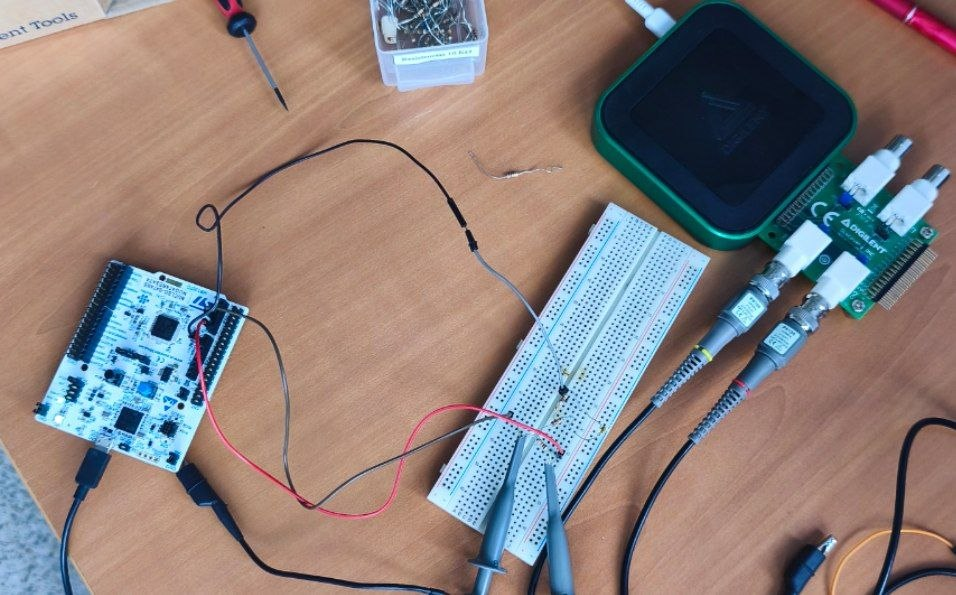
\includegraphics[width=0.85\textwidth]{montaje.jpg}
    \caption{Montaje experimental utilizado durante las pruebas con la Analog Discovery 3 de Digilent.}
    \label{fig:montaje-analog-discovery}
\end{figure}

\begin{figure}[H]
\centering
\begin{tikzpicture}[x=1cm,y=1cm, thick]
    \draw (0,0) node[left] {\(V_A\)} -- (0.6,0);
    \draw (0.6,0) -- (0.85,0.25) -- (1.1,-0.25) -- (1.35,0.25) -- (1.6,-0.25) -- (1.85,0.25) -- (2.1,0);
    \node[above] at (1.35,0.55) {\(R_1=10~k\Omega\)};
    \draw (2.1,0) -- (2.8,0);
    \filldraw (2.8,0) circle (1.4pt);
    \node[above] at (2.8,0.18) {\(V_B\)};
    \draw (2.8,0) -- (3.05,0.25) -- (3.3,-0.25) -- (3.55,0.25) -- (3.8,-0.25) -- (4.05,0.25) -- (4.3,0);
    \node[above] at (3.55,0.55) {\(R_2=10~k\Omega\)};
    \draw (4.3,0) -- (5.0,0);
    \draw (5.0,0) -- (5.8,0);
    \draw (5.8,0) -- (6.05,0.25) -- (6.3,-0.25) -- (6.55,0.25) -- (6.8,-0.25) -- (7.05,0.25) -- (7.3,0);
    \node[above] at (6.55,0.55) {\(R_3=10~k\Omega\)};
    \draw (7.3,0) -- (8.1,0) -- (8.1,-1.9);
    \draw (2.8,0) -- (2.8,-1.2) -- (6.15,-1.2);
    \draw (6.15,-0.75) -- (6.15,-1.65);
    \draw (6.45,-0.75) -- (6.45,-1.65);
    \draw (6.45,-1.2) -- (8.1,-1.2);
    \node[below] at (6.3,-1.65) {\(C=10~nF\)};
    \draw (8.1,-1.9) -- (7.65,-1.9) -- (8.55,-1.9);
    \draw (7.78,-2.12) -- (8.42,-2.12);
    \draw (7.92,-2.34) -- (8.28,-2.34);
\end{tikzpicture}
\caption{Circuito de prueba utilizado para las medidas de impedancia.}
\label{fig:circuito-prueba-rc}
\end{figure}

\myparagraph{Formas de onda observadas}

Antes de aplicar el modelo eléctrico, se representaron las formas de onda registradas en cada ensayo. En las Figuras~\ref{fig:ondas-medidas-baja}, \ref{fig:ondas-medidas-media} y \ref{fig:ondas-medidas-alta} se muestran dos periodos de los canales \(V_A\) y \(V_B\). Para facilitar la comparación se eliminó únicamente el valor medio de cada canal y se mantuvo una escala vertical común de \(\pm 1.8~V\). Por tanto, las gráficas conservan tanto la relación de amplitudes como el desplazamiento temporal entre ambas señales.

El eje horizontal se expresa en ciclos de la señal y no en segundos, lo que permite comparar en una misma escala capturas realizadas desde décimas de hercio hasta decenas de kilohercios. Sobre cada caso se indican la frecuencia medida, la ganancia \(\lvert V_B/V_A\rvert\) y el desfase calculado a partir de la captura completa.

% Formas de onda generadas automaticamente por scripts/analyze_medidas.ps1
\begin{figure}[H]
\centering
\begin{minipage}[t]{0.46\textwidth}
\centering
{\scriptsize \(f=0.47~Hz,\quad |H|=0.663,\quad \Delta\phi=0.0^\circ\)}\\[0.4em]
\begin{tikzpicture}[x=2.25cm,y=1.0cm]
\draw[gray!20] (0,-1.8) grid[xstep=0.5,ystep=0.6] (2,1.8);
\draw[gray!55] (0,0) -- (2,0);
\draw[->] (0,-1.8) -- (2.08,-1.8) node[right, font=\scriptsize] {ciclos};
\draw[->] (0,-1.8) -- (0,2.05) node[above, font=\scriptsize] {V};
\node[left, font=\tiny] at (0,-1.8) {-1.8};
\node[left, font=\tiny] at (0,0) {0};
\node[left, font=\tiny] at (0,1.8) {1.8};
\foreach \x in {0.5,1,1.5,2} {
    \node[below, font=\tiny] at (\x,-1.8) {\x};
}
\draw[very thick, blue!70!black] (0.0000,0.0015) -- (0.0148,0.0024) -- (0.0295,0.0033) -- (0.0443,0.3215) -- (0.0590,0.3224) -- (0.0738,0.6263) -- (0.0885,0.6272) -- (0.1033,0.9086) -- (0.1181,0.9095) -- (0.1328,1.1567) -- (0.1476,1.1567) -- (0.1623,1.3599) -- (0.1771,1.3590) -- (0.1918,1.5109) -- (0.2066,1.5082) -- (0.2214,1.6026) -- (0.2361,1.6017) -- (0.2509,1.6350) -- (0.2656,1.6341) -- (0.2804,1.6332) -- (0.2951,1.6008) -- (0.3099,1.6017) -- (0.3246,1.5082) -- (0.3394,1.5100) -- (0.3542,1.3581) -- (0.3689,1.3590) -- (0.3837,1.1558) -- (0.3984,1.1549) -- (0.4132,0.9077) -- (0.4279,0.9086) -- (0.4427,0.6272) -- (0.4575,0.6281) -- (0.4722,0.3224) -- (0.4870,0.3224) -- (0.5017,0.0033) -- (0.5165,0.0024) -- (0.5312,-0.3123) -- (0.5460,-0.3141) -- (0.5608,-0.3141) -- (0.5755,-0.6188) -- (0.5903,-0.6197) -- (0.6050,-0.9020) -- (0.6198,-0.9029) -- (0.6345,-1.1484) -- (0.6493,-1.1475) -- (0.6641,-1.3524) -- (0.6788,-1.3524) -- (0.6936,-1.5026) -- (0.7083,-1.5008) -- (0.7231,-1.5862) -- (0.7378,-1.5862) -- (0.7526,-1.5862) -- (0.7673,-1.5862) -- (0.7821,-1.5871) -- (0.7969,-1.5871) -- (0.8116,-1.5871) -- (0.8264,-1.5017) -- (0.8411,-1.5026) -- (0.8559,-1.3515) -- (0.8706,-1.3515) -- (0.8854,-1.1466) -- (0.9002,-1.1475) -- (0.9149,-0.9020) -- (0.9297,-0.9020) -- (0.9444,-0.6206) -- (0.9592,-0.6197) -- (0.9739,-0.3141) -- (0.9887,-0.3150) -- (1.0035,0.0024) -- (1.0182,0.0024) -- (1.0330,0.3224) -- (1.0477,0.3233) -- (1.0625,0.6281) -- (1.0772,0.6272) -- (1.0920,0.6272) -- (1.1068,0.9077) -- (1.1215,0.9086) -- (1.1363,1.1567) -- (1.1510,1.1558) -- (1.1658,1.3581) -- (1.1805,1.3590) -- (1.1953,1.5082) -- (1.2100,1.5091) -- (1.2248,1.6026) -- (1.2396,1.6017) -- (1.2543,1.6341) -- (1.2691,1.6332) -- (1.2838,1.6017) -- (1.2986,1.6017) -- (1.3133,1.5091) -- (1.3281,1.5091) -- (1.3429,1.5100) -- (1.3576,1.3590) -- (1.3724,1.3590) -- (1.3871,1.1558) -- (1.4019,1.1558) -- (1.4166,0.9086) -- (1.4314,0.9086) -- (1.4462,0.6272) -- (1.4609,0.6281) -- (1.4757,0.3233) -- (1.4904,0.3224) -- (1.5052,0.0033) -- (1.5199,0.0033) -- (1.5347,-0.3132) -- (1.5495,-0.3132) -- (1.5642,-0.6197) -- (1.5790,-0.6188) -- (1.5937,-0.9011) -- (1.6085,-0.9020) -- (1.6232,-0.9029) -- (1.6380,-1.1457) -- (1.6528,-1.1475) -- (1.6675,-1.3506) -- (1.6823,-1.3515) -- (1.6970,-1.5017) -- (1.7118,-1.5017) -- (1.7265,-1.5871) -- (1.7413,-1.5862) -- (1.7560,-1.5862) -- (1.7708,-1.5862) -- (1.7856,-1.5871) -- (1.8003,-1.5871) -- (1.8151,-1.5008) -- (1.8298,-1.5017) -- (1.8446,-1.3515) -- (1.8593,-1.3506) -- (1.8741,-1.3506) -- (1.8889,-1.1475) -- (1.9036,-1.1475) -- (1.9184,-0.9020) -- (1.9331,-0.9020) -- (1.9479,-0.6206) -- (1.9626,-0.6206) -- (1.9774,-0.3132) -- (1.9922,-0.3132);
\draw[very thick, orange!85!black] (0.0000,0.0013) -- (0.0148,0.0013) -- (0.0295,0.0013) -- (0.0443,0.2131) -- (0.0590,0.2122) -- (0.0738,0.4159) -- (0.0885,0.4159) -- (0.1033,0.6016) -- (0.1181,0.6025) -- (0.1328,0.7675) -- (0.1476,0.7675) -- (0.1623,0.9000) -- (0.1771,0.9000) -- (0.1918,1.0018) -- (0.2066,1.0009) -- (0.2214,1.0631) -- (0.2361,1.0622) -- (0.2509,1.0820) -- (0.2656,1.0820) -- (0.2804,1.0811) -- (0.2951,1.0622) -- (0.3099,1.0622) -- (0.3246,1.0009) -- (0.3394,1.0018) -- (0.3542,0.9009) -- (0.3689,0.9009) -- (0.3837,0.7666) -- (0.3984,0.7675) -- (0.4132,0.6025) -- (0.4279,0.6016) -- (0.4427,0.4150) -- (0.4575,0.4159) -- (0.4722,0.2131) -- (0.4870,0.2122) -- (0.5017,0.0013) -- (0.5165,0.0013) -- (0.5312,-0.2087) -- (0.5460,-0.2087) -- (0.5608,-0.2087) -- (0.5755,-0.4115) -- (0.5903,-0.4124) -- (0.6050,-0.5972) -- (0.6198,-0.5972) -- (0.6345,-0.7630) -- (0.6493,-0.7639) -- (0.6641,-0.8973) -- (0.6788,-0.8973) -- (0.6936,-0.9965) -- (0.7083,-0.9965) -- (0.7231,-1.0523) -- (0.7378,-1.0523) -- (0.7526,-1.0523) -- (0.7673,-1.0523) -- (0.7821,-1.0523) -- (0.7969,-1.0523) -- (0.8116,-1.0532) -- (0.8264,-0.9956) -- (0.8411,-0.9956) -- (0.8559,-0.8973) -- (0.8706,-0.8973) -- (0.8854,-0.7630) -- (0.9002,-0.7621) -- (0.9149,-0.5963) -- (0.9297,-0.5972) -- (0.9444,-0.4106) -- (0.9592,-0.4106) -- (0.9739,-0.2078) -- (0.9887,-0.2096) -- (1.0035,0.0022) -- (1.0182,0.0031) -- (1.0330,0.2131) -- (1.0477,0.2131) -- (1.0625,0.4168) -- (1.0772,0.4159) -- (1.0920,0.4159) -- (1.1068,0.6025) -- (1.1215,0.6016) -- (1.1363,0.7666) -- (1.1510,0.7675) -- (1.1658,0.9018) -- (1.1805,0.9009) -- (1.1953,1.0009) -- (1.2100,1.0018) -- (1.2248,1.0631) -- (1.2396,1.0622) -- (1.2543,1.0820) -- (1.2691,1.0820) -- (1.2838,1.0631) -- (1.2986,1.0640) -- (1.3133,1.0018) -- (1.3281,1.0018) -- (1.3429,1.0009) -- (1.3576,0.9027) -- (1.3724,0.9018) -- (1.3871,0.7675) -- (1.4019,0.7666) -- (1.4166,0.6025) -- (1.4314,0.6025) -- (1.4462,0.4150) -- (1.4609,0.4159) -- (1.4757,0.2122) -- (1.4904,0.2131) -- (1.5052,0.0022) -- (1.5199,0.0013) -- (1.5347,-0.2078) -- (1.5495,-0.2087) -- (1.5642,-0.4115) -- (1.5790,-0.4106) -- (1.5937,-0.5963) -- (1.6085,-0.5963) -- (1.6232,-0.5972) -- (1.6380,-0.7621) -- (1.6528,-0.7621) -- (1.6675,-0.8973) -- (1.6823,-0.8973) -- (1.6970,-0.9956) -- (1.7118,-0.9956) -- (1.7265,-1.0523) -- (1.7413,-1.0523) -- (1.7560,-1.0505) -- (1.7708,-1.0514) -- (1.7856,-1.0532) -- (1.8003,-1.0514) -- (1.8151,-0.9965) -- (1.8298,-0.9965) -- (1.8446,-0.8973) -- (1.8593,-0.8973) -- (1.8741,-0.8973) -- (1.8889,-0.7621) -- (1.9036,-0.7621) -- (1.9184,-0.5972) -- (1.9331,-0.5981) -- (1.9479,-0.4097) -- (1.9626,-0.4124) -- (1.9774,-0.2096) -- (1.9922,-0.2087);
\draw[very thick, blue!70!black] (0.08,1.62) -- (0.30,1.62);
\node[right, font=\tiny] at (0.30,1.62) {\(V_A\)};
\draw[very thick, orange!85!black] (0.72,1.62) -- (0.94,1.62);
\node[right, font=\tiny] at (0.94,1.62) {\(V_B\)};
\end{tikzpicture}
\end{minipage}
\hfill
\begin{minipage}[t]{0.46\textwidth}
\centering
{\scriptsize \(f=4.72~Hz,\quad |H|=0.663,\quad \Delta\phi=0.0^\circ\)}\\[0.4em]
\begin{tikzpicture}[x=2.25cm,y=1.0cm]
\draw[gray!20] (0,-1.8) grid[xstep=0.5,ystep=0.6] (2,1.8);
\draw[gray!55] (0,0) -- (2,0);
\draw[->] (0,-1.8) -- (2.08,-1.8) node[right, font=\scriptsize] {ciclos};
\draw[->] (0,-1.8) -- (0,2.05) node[above, font=\scriptsize] {V};
\node[left, font=\tiny] at (0,-1.8) {-1.8};
\node[left, font=\tiny] at (0,0) {0};
\node[left, font=\tiny] at (0,1.8) {1.8};
\foreach \x in {0.5,1,1.5,2} {
    \node[below, font=\tiny] at (\x,-1.8) {\x};
}
\draw[very thick, blue!70!black] (0.0000,0.0733) -- (0.0147,0.3007) -- (0.0295,0.3007) -- (0.0442,0.6046) -- (0.0590,0.6046) -- (0.0737,0.8869) -- (0.0885,0.8878) -- (0.1032,1.1341) -- (0.1180,1.1341) -- (0.1327,1.3364) -- (0.1475,1.3373) -- (0.1622,1.4865) -- (0.1770,1.4874) -- (0.1917,1.5809) -- (0.2065,1.5800) -- (0.2212,1.6115) -- (0.2360,1.6124) -- (0.2507,1.5872) -- (0.2655,1.5800) -- (0.2802,1.5809) -- (0.2950,1.4865) -- (0.3097,1.4865) -- (0.3245,1.3364) -- (0.3392,1.3355) -- (0.3540,1.1341) -- (0.3687,1.1341) -- (0.3835,0.8842) -- (0.3982,0.8860) -- (0.4130,0.6064) -- (0.4277,0.6064) -- (0.4425,0.3016) -- (0.4572,0.3007) -- (0.4720,-0.0184) -- (0.4867,-0.0175) -- (0.5015,-0.3358) -- (0.5162,-0.3358) -- (0.5310,-0.3574) -- (0.5457,-0.6414) -- (0.5605,-0.6414) -- (0.5752,-0.9228) -- (0.5900,-0.9228) -- (0.6047,-1.1674) -- (0.6195,-1.1665) -- (0.6342,-1.3723) -- (0.6490,-1.3714) -- (0.6637,-1.5225) -- (0.6785,-1.5225) -- (0.6932,-1.6088) -- (0.7080,-1.6088) -- (0.7227,-1.6070) -- (0.7375,-1.6079) -- (0.7522,-1.6079) -- (0.7670,-1.6097) -- (0.7817,-1.5611) -- (0.7965,-1.5225) -- (0.8112,-1.5225) -- (0.8260,-1.3723) -- (0.8407,-1.3723) -- (0.8555,-1.1683) -- (0.8702,-1.1674) -- (0.8850,-0.9237) -- (0.8997,-0.9237) -- (0.9145,-0.6405) -- (0.9292,-0.6405) -- (0.9440,-0.3349) -- (0.9587,-0.3349) -- (0.9734,-0.0184) -- (0.9882,-0.0193) -- (1.0029,0.2998) -- (1.0177,0.2998) -- (1.0324,0.6064) -- (1.0472,0.6055) -- (1.0619,0.6073) -- (1.0767,0.8860) -- (1.0914,0.8878) -- (1.1062,1.1350) -- (1.1209,1.1350) -- (1.1357,1.3373) -- (1.1504,1.3364) -- (1.1652,1.4883) -- (1.1799,1.4865) -- (1.1947,1.5809) -- (1.2094,1.5809) -- (1.2242,1.6115) -- (1.2389,1.6124) -- (1.2537,1.5800) -- (1.2684,1.5800) -- (1.2832,1.4883) -- (1.2979,1.4892) -- (1.3127,1.4308) -- (1.3274,1.3373) -- (1.3422,1.3364) -- (1.3569,1.1341) -- (1.3717,1.1350) -- (1.3864,0.8878) -- (1.4012,0.8878) -- (1.4159,0.6055) -- (1.4307,0.6055) -- (1.4454,0.3016) -- (1.4602,0.3007) -- (1.4749,-0.0175) -- (1.4897,-0.0175) -- (1.5044,-0.3349) -- (1.5192,-0.3340) -- (1.5339,-0.6405) -- (1.5487,-0.6414) -- (1.5634,-0.8941) -- (1.5782,-0.9228) -- (1.5929,-0.9237) -- (1.6077,-1.1692) -- (1.6224,-1.1683) -- (1.6372,-1.3714) -- (1.6519,-1.3714) -- (1.6667,-1.5225) -- (1.6814,-1.5225) -- (1.6962,-1.6079) -- (1.7109,-1.6079) -- (1.7257,-1.6070) -- (1.7404,-1.6079) -- (1.7552,-1.6088) -- (1.7699,-1.6088) -- (1.7847,-1.5234) -- (1.7994,-1.5243) -- (1.8142,-1.3723) -- (1.8289,-1.3714) -- (1.8437,-1.3256) -- (1.8584,-1.1683) -- (1.8732,-1.1683) -- (1.8879,-0.9228) -- (1.9026,-0.9228) -- (1.9174,-0.6414) -- (1.9321,-0.6414) -- (1.9469,-0.3349) -- (1.9616,-0.3349) -- (1.9764,-0.0184) -- (1.9911,-0.0193);
\draw[very thick, orange!85!black] (0.0000,0.0466) -- (0.0147,0.1981) -- (0.0295,0.1990) -- (0.0442,0.4018) -- (0.0590,0.4018) -- (0.0737,0.5883) -- (0.0885,0.5874) -- (0.1032,0.7533) -- (0.1180,0.7533) -- (0.1327,0.8876) -- (0.1475,0.8867) -- (0.1622,0.9876) -- (0.1770,0.9876) -- (0.1917,1.0489) -- (0.2065,1.0489) -- (0.2212,1.0678) -- (0.2360,1.0687) -- (0.2507,1.0525) -- (0.2655,1.0471) -- (0.2802,1.0489) -- (0.2950,0.9867) -- (0.3097,0.9876) -- (0.3245,0.8867) -- (0.3392,0.8867) -- (0.3540,0.7533) -- (0.3687,0.7533) -- (0.3835,0.5865) -- (0.3982,0.5883) -- (0.4130,0.4018) -- (0.4277,0.4027) -- (0.4425,0.1990) -- (0.4572,0.1981) -- (0.4720,-0.0129) -- (0.4867,-0.0111) -- (0.5015,-0.2220) -- (0.5162,-0.2220) -- (0.5310,-0.2364) -- (0.5457,-0.4248) -- (0.5605,-0.4248) -- (0.5752,-0.6113) -- (0.5900,-0.6113) -- (0.6047,-0.7772) -- (0.6195,-0.7763) -- (0.6342,-0.9106) -- (0.6490,-0.9106) -- (0.6637,-1.0097) -- (0.6785,-1.0079) -- (0.6932,-1.0656) -- (0.7080,-1.0656) -- (0.7227,-1.0656) -- (0.7375,-1.0656) -- (0.7522,-1.0647) -- (0.7670,-1.0656) -- (0.7817,-1.0332) -- (0.7965,-1.0088) -- (0.8112,-1.0088) -- (0.8260,-0.9097) -- (0.8407,-0.9106) -- (0.8555,-0.7754) -- (0.8702,-0.7763) -- (0.8850,-0.6104) -- (0.8997,-0.6104) -- (0.9145,-0.4248) -- (0.9292,-0.4248) -- (0.9440,-0.2229) -- (0.9587,-0.2220) -- (0.9734,-0.0111) -- (0.9882,-0.0120) -- (1.0029,0.1990) -- (1.0177,0.1990) -- (1.0324,0.4018) -- (1.0472,0.4018) -- (1.0619,0.4027) -- (1.0767,0.5883) -- (1.0914,0.5892) -- (1.1062,0.7533) -- (1.1209,0.7533) -- (1.1357,0.8876) -- (1.1504,0.8867) -- (1.1652,0.9876) -- (1.1799,0.9858) -- (1.1947,1.0480) -- (1.2094,1.0480) -- (1.2242,1.0669) -- (1.2389,1.0669) -- (1.2537,1.0480) -- (1.2684,1.0471) -- (1.2832,0.9867) -- (1.2979,0.9876) -- (1.3127,0.9489) -- (1.3274,0.8876) -- (1.3422,0.8867) -- (1.3569,0.7524) -- (1.3717,0.7524) -- (1.3864,0.5883) -- (1.4012,0.5883) -- (1.4159,0.4018) -- (1.4307,0.4009) -- (1.4454,0.1981) -- (1.4602,0.1990) -- (1.4749,-0.0120) -- (1.4897,-0.0129) -- (1.5044,-0.2238) -- (1.5192,-0.2229) -- (1.5339,-0.4257) -- (1.5487,-0.4248) -- (1.5634,-0.5906) -- (1.5782,-0.6113) -- (1.5929,-0.6113) -- (1.6077,-0.7772) -- (1.6224,-0.7763) -- (1.6372,-0.9106) -- (1.6519,-0.9106) -- (1.6667,-1.0097) -- (1.6814,-1.0106) -- (1.6962,-1.0656) -- (1.7109,-1.0674) -- (1.7257,-1.0665) -- (1.7404,-1.0656) -- (1.7552,-1.0665) -- (1.7699,-1.0656) -- (1.7847,-1.0088) -- (1.7994,-1.0097) -- (1.8142,-0.9106) -- (1.8289,-0.9106) -- (1.8437,-0.8808) -- (1.8584,-0.7772) -- (1.8732,-0.7772) -- (1.8879,-0.6113) -- (1.9026,-0.6113) -- (1.9174,-0.4248) -- (1.9321,-0.4248) -- (1.9469,-0.2229) -- (1.9616,-0.2229) -- (1.9764,-0.0120) -- (1.9911,-0.0120);
\draw[very thick, blue!70!black] (0.08,1.62) -- (0.30,1.62);
\node[right, font=\tiny] at (0.30,1.62) {\(V_A\)};
\draw[very thick, orange!85!black] (0.72,1.62) -- (0.94,1.62);
\node[right, font=\tiny] at (0.94,1.62) {\(V_B\)};
\end{tikzpicture}
\end{minipage}
\par\medskip
\begin{minipage}[t]{0.46\textwidth}
\centering
{\scriptsize \(f=9.42~Hz,\quad |H|=0.703,\quad \Delta\phi=0.0^\circ\)}\\[0.4em]
\begin{tikzpicture}[x=2.25cm,y=1.0cm]
\draw[gray!20] (0,-1.8) grid[xstep=0.5,ystep=0.6] (2,1.8);
\draw[gray!55] (0,0) -- (2,0);
\draw[->] (0,-1.8) -- (2.08,-1.8) node[right, font=\scriptsize] {ciclos};
\draw[->] (0,-1.8) -- (0,2.05) node[above, font=\scriptsize] {V};
\node[left, font=\tiny] at (0,-1.8) {-1.8};
\node[left, font=\tiny] at (0,0) {0};
\node[left, font=\tiny] at (0,1.8) {1.8};
\foreach \x in {0.5,1,1.5,2} {
    \node[below, font=\tiny] at (\x,-1.8) {\x};
}
\draw[very thick, blue!70!black] (0.0000,0.2259) -- (0.0153,0.2852) -- (0.0306,0.3643) -- (0.0459,0.5738) -- (0.0613,0.5729) -- (0.0766,0.8426) -- (0.0919,0.8399) -- (0.1072,1.0755) -- (0.1225,1.0755) -- (0.1378,1.2706) -- (0.1531,1.2697) -- (0.1685,1.4135) -- (0.1838,1.4153) -- (0.1991,1.5043) -- (0.2144,1.5007) -- (0.2297,1.5322) -- (0.2450,1.5331) -- (0.2603,1.5043) -- (0.2757,1.5016) -- (0.2910,1.4135) -- (0.3063,1.4162) -- (0.3216,1.2706) -- (0.3369,1.2697) -- (0.3522,1.0737) -- (0.3676,1.0782) -- (0.3829,0.8408) -- (0.3982,0.8417) -- (0.4135,0.5729) -- (0.4288,0.5702) -- (0.4441,0.2852) -- (0.4594,0.2861) -- (0.4748,-0.0177) -- (0.4901,-0.0177) -- (0.5054,-0.3171) -- (0.5207,-0.3162) -- (0.5360,-0.6039) -- (0.5513,-0.6030) -- (0.5666,-0.8664) -- (0.5820,-0.8655) -- (0.5973,-1.0939) -- (0.6126,-1.0948) -- (0.6279,-1.2845) -- (0.6432,-1.2845) -- (0.6585,-1.4247) -- (0.6738,-1.4238) -- (0.6892,-1.5038) -- (0.7045,-1.5038) -- (0.7198,-1.5047) -- (0.7351,-1.5047) -- (0.7504,-1.5038) -- (0.7657,-1.5029) -- (0.7810,-1.4373) -- (0.7964,-1.4238) -- (0.8117,-1.3780) -- (0.8270,-1.2845) -- (0.8423,-1.2836) -- (0.8576,-1.0957) -- (0.8729,-1.0957) -- (0.8882,-0.8646) -- (0.9036,-0.8646) -- (0.9189,-0.6021) -- (0.9342,-0.6021) -- (0.9495,-0.3162) -- (0.9648,-0.3144) -- (0.9801,-0.0177) -- (0.9955,-0.0177) -- (1.0108,0.2852) -- (1.0261,0.2870) -- (1.0414,0.5738) -- (1.0567,0.5747) -- (1.0720,0.8408) -- (1.0873,0.8408) -- (1.1027,1.0791) -- (1.1180,1.0773) -- (1.1333,1.2733) -- (1.1486,1.2715) -- (1.1639,1.4180) -- (1.1792,1.4144) -- (1.1945,1.5034) -- (1.2099,1.5034) -- (1.2252,1.5358) -- (1.2405,1.5340) -- (1.2558,1.5070) -- (1.2711,1.4998) -- (1.2864,1.4153) -- (1.3017,1.4135) -- (1.3171,1.2706) -- (1.3324,1.2715) -- (1.3477,1.0737) -- (1.3630,1.0737) -- (1.3783,0.8426) -- (1.3936,0.8399) -- (1.4089,0.5720) -- (1.4243,0.5729) -- (1.4396,0.2870) -- (1.4549,0.2879) -- (1.4702,-0.0177) -- (1.4855,-0.0168) -- (1.5008,-0.3153) -- (1.5161,-0.3153) -- (1.5315,-0.6021) -- (1.5468,-0.6012) -- (1.5621,-0.8412) -- (1.5774,-0.8655) -- (1.5927,-0.9545) -- (1.6080,-1.0948) -- (1.6234,-1.0957) -- (1.6387,-1.2845) -- (1.6540,-1.2845) -- (1.6693,-1.4247) -- (1.6846,-1.4247) -- (1.6999,-1.5047) -- (1.7152,-1.5038) -- (1.7306,-1.5029) -- (1.7459,-1.5038) -- (1.7612,-1.5056) -- (1.7765,-1.5038) -- (1.7918,-1.4247) -- (1.8071,-1.4247) -- (1.8224,-1.2845) -- (1.8378,-1.2836) -- (1.8531,-1.0939) -- (1.8684,-1.0957) -- (1.8837,-0.8655) -- (1.8990,-0.8664) -- (1.9143,-0.6012) -- (1.9296,-0.6003) -- (1.9450,-0.3153) -- (1.9603,-0.3144) -- (1.9756,-0.0177) -- (1.9909,-0.0177);
\draw[very thick, orange!85!black] (0.0000,0.1650) -- (0.0153,0.2020) -- (0.0306,0.2642) -- (0.0459,0.4066) -- (0.0613,0.4057) -- (0.0766,0.5941) -- (0.0919,0.5941) -- (0.1072,0.7581) -- (0.1225,0.7572) -- (0.1378,0.8906) -- (0.1531,0.8915) -- (0.1685,0.9915) -- (0.1838,0.9915) -- (0.1991,1.0546) -- (0.2144,1.0537) -- (0.2297,1.0736) -- (0.2450,1.0736) -- (0.2603,1.0528) -- (0.2757,1.0528) -- (0.2910,0.9906) -- (0.3063,0.9924) -- (0.3216,0.8924) -- (0.3369,0.8915) -- (0.3522,0.7572) -- (0.3676,0.7572) -- (0.3829,0.5941) -- (0.3982,0.5941) -- (0.4135,0.4066) -- (0.4288,0.4066) -- (0.4441,0.2029) -- (0.4594,0.2029) -- (0.4748,-0.0062) -- (0.4901,-0.0062) -- (0.5054,-0.2153) -- (0.5207,-0.2171) -- (0.5360,-0.4208) -- (0.5513,-0.4199) -- (0.5666,-0.6065) -- (0.5820,-0.6065) -- (0.5973,-0.7724) -- (0.6126,-0.7715) -- (0.6279,-0.9067) -- (0.6432,-0.9067) -- (0.6585,-1.0049) -- (0.6738,-1.0049) -- (0.6892,-1.0599) -- (0.7045,-1.0608) -- (0.7198,-1.0599) -- (0.7351,-1.0608) -- (0.7504,-1.0617) -- (0.7657,-1.0617) -- (0.7810,-1.0121) -- (0.7964,-1.0058) -- (0.8117,-0.9689) -- (0.8270,-0.9058) -- (0.8423,-0.9067) -- (0.8576,-0.7733) -- (0.8729,-0.7724) -- (0.8882,-0.6056) -- (0.9036,-0.6065) -- (0.9189,-0.4199) -- (0.9342,-0.4208) -- (0.9495,-0.2162) -- (0.9648,-0.2180) -- (0.9801,-0.0071) -- (0.9955,-0.0071) -- (1.0108,0.2038) -- (1.0261,0.2029) -- (1.0414,0.4066) -- (1.0567,0.4057) -- (1.0720,0.5932) -- (1.0873,0.5941) -- (1.1027,0.7581) -- (1.1180,0.7572) -- (1.1333,0.8933) -- (1.1486,0.8915) -- (1.1639,0.9933) -- (1.1792,0.9915) -- (1.1945,1.0528) -- (1.2099,1.0519) -- (1.2252,1.0727) -- (1.2405,1.0727) -- (1.2558,1.0528) -- (1.2711,1.0528) -- (1.2864,0.9906) -- (1.3017,0.9906) -- (1.3171,0.8915) -- (1.3324,0.8915) -- (1.3477,0.7563) -- (1.3630,0.7563) -- (1.3783,0.5941) -- (1.3936,0.5941) -- (1.4089,0.4066) -- (1.4243,0.4075) -- (1.4396,0.2029) -- (1.4549,0.2020) -- (1.4702,-0.0062) -- (1.4855,-0.0053) -- (1.5008,-0.2162) -- (1.5161,-0.2171) -- (1.5315,-0.4190) -- (1.5468,-0.4199) -- (1.5621,-0.5984) -- (1.5774,-0.6065) -- (1.5927,-0.6786) -- (1.6080,-0.7706) -- (1.6234,-0.7715) -- (1.6387,-0.9058) -- (1.6540,-0.9049) -- (1.6693,-1.0049) -- (1.6846,-1.0049) -- (1.6999,-1.0608) -- (1.7152,-1.0608) -- (1.7306,-1.0608) -- (1.7459,-1.0599) -- (1.7612,-1.0608) -- (1.7765,-1.0599) -- (1.7918,-1.0040) -- (1.8071,-1.0040) -- (1.8224,-0.9067) -- (1.8378,-0.9067) -- (1.8531,-0.7715) -- (1.8684,-0.7724) -- (1.8837,-0.6065) -- (1.8990,-0.6065) -- (1.9143,-0.4199) -- (1.9296,-0.4208) -- (1.9450,-0.2180) -- (1.9603,-0.2171) -- (1.9756,-0.0062) -- (1.9909,-0.0062);
\draw[very thick, blue!70!black] (0.08,1.62) -- (0.30,1.62);
\node[right, font=\tiny] at (0.30,1.62) {\(V_A\)};
\draw[very thick, orange!85!black] (0.72,1.62) -- (0.94,1.62);
\node[right, font=\tiny] at (0.94,1.62) {\(V_B\)};
\end{tikzpicture}
\end{minipage}
\hfill
\begin{minipage}[t]{0.46\textwidth}
\centering
{\scriptsize \(f=23.60~Hz,\quad |H|=0.732,\quad \Delta\phi=0.1^\circ\)}\\[0.4em]
\begin{tikzpicture}[x=2.25cm,y=1.0cm]
\draw[gray!20] (0,-1.8) grid[xstep=0.5,ystep=0.6] (2,1.8);
\draw[gray!55] (0,0) -- (2,0);
\draw[->] (0,-1.8) -- (2.08,-1.8) node[right, font=\scriptsize] {ciclos};
\draw[->] (0,-1.8) -- (0,2.05) node[above, font=\scriptsize] {V};
\node[left, font=\tiny] at (0,-1.8) {-1.8};
\node[left, font=\tiny] at (0,0) {0};
\node[left, font=\tiny] at (0,1.8) {1.8};
\foreach \x in {0.5,1,1.5,2} {
    \node[below, font=\tiny] at (\x,-1.8) {\x};
}
\draw[very thick, blue!70!black] (0.0000,0.0026) -- (0.0148,0.2813) -- (0.0295,0.2804) -- (0.0443,0.5654) -- (0.0590,0.5654) -- (0.0738,0.8279) -- (0.0885,0.8270) -- (0.1033,1.0536) -- (0.1180,1.0536) -- (0.1328,1.2460) -- (0.1475,1.2433) -- (0.1623,1.3862) -- (0.1770,1.3835) -- (0.1918,1.4716) -- (0.2065,1.4716) -- (0.2213,1.5031) -- (0.2360,1.5040) -- (0.2508,1.4752) -- (0.2655,1.4725) -- (0.2803,1.4716) -- (0.2950,1.3853) -- (0.3098,1.3862) -- (0.3245,1.2442) -- (0.3393,1.2433) -- (0.3540,1.0491) -- (0.3688,1.0518) -- (0.3835,0.8198) -- (0.3983,0.8198) -- (0.4130,0.5600) -- (0.4278,0.5591) -- (0.4425,0.2741) -- (0.4573,0.2759) -- (0.4720,-0.0153) -- (0.4868,-0.0153) -- (0.5015,-0.2967) -- (0.5163,-0.3048) -- (0.5310,-0.3048) -- (0.5458,-0.5817) -- (0.5605,-0.5808) -- (0.5753,-0.8325) -- (0.5900,-0.8308) -- (0.6048,-1.0420) -- (0.6195,-1.0420) -- (0.6343,-1.2146) -- (0.6490,-1.2137) -- (0.6638,-1.3387) -- (0.6785,-1.3387) -- (0.6933,-1.4115) -- (0.7081,-1.4106) -- (0.7228,-1.4106) -- (0.7376,-1.4106) -- (0.7523,-1.4097) -- (0.7671,-1.4106) -- (0.7818,-1.3738) -- (0.7966,-1.3405) -- (0.8113,-1.3396) -- (0.8261,-1.2146) -- (0.8408,-1.2146) -- (0.8556,-1.0411) -- (0.8703,-1.0411) -- (0.8851,-0.8290) -- (0.8998,-0.8299) -- (0.9146,-0.5781) -- (0.9293,-0.5781) -- (0.9441,-0.3030) -- (0.9588,-0.3039) -- (0.9736,-0.0171) -- (0.9883,-0.0153) -- (1.0031,0.2768) -- (1.0178,0.2750) -- (1.0326,0.5582) -- (1.0473,0.5555) -- (1.0621,0.5582) -- (1.0768,0.8189) -- (1.0916,0.8216) -- (1.1063,1.0509) -- (1.1211,1.0491) -- (1.1358,1.2406) -- (1.1506,1.2406) -- (1.1653,1.3817) -- (1.1801,1.3808) -- (1.1948,1.4698) -- (1.2096,1.4689) -- (1.2243,1.4995) -- (1.2391,1.4959) -- (1.2538,1.4680) -- (1.2686,1.4680) -- (1.2833,1.3835) -- (1.2981,1.3826) -- (1.3128,1.3206) -- (1.3276,1.2379) -- (1.3423,1.2370) -- (1.3571,1.0464) -- (1.3718,1.0464) -- (1.3866,0.8172) -- (1.4014,0.8163) -- (1.4161,0.5573) -- (1.4309,0.5573) -- (1.4456,0.2741) -- (1.4604,0.2705) -- (1.4751,-0.0189) -- (1.4899,-0.0207) -- (1.5046,-0.3093) -- (1.5194,-0.3093) -- (1.5341,-0.5808) -- (1.5489,-0.5826) -- (1.5636,-0.7984) -- (1.5784,-0.8334) -- (1.5931,-0.8317) -- (1.6079,-1.0429) -- (1.6226,-1.0447) -- (1.6374,-1.2155) -- (1.6521,-1.2155) -- (1.6669,-1.3387) -- (1.6816,-1.3405) -- (1.6964,-1.4097) -- (1.7111,-1.4106) -- (1.7259,-1.4097) -- (1.7406,-1.4106) -- (1.7554,-1.4106) -- (1.7701,-1.4097) -- (1.7849,-1.3387) -- (1.7996,-1.3405) -- (1.8144,-1.2173) -- (1.8291,-1.2137) -- (1.8439,-1.1661) -- (1.8586,-1.0411) -- (1.8734,-1.0420) -- (1.8881,-0.8290) -- (1.9029,-0.8281) -- (1.9176,-0.5808) -- (1.9324,-0.5790) -- (1.9471,-0.3039) -- (1.9619,-0.3057) -- (1.9766,-0.0198) -- (1.9914,-0.0153);
\draw[very thick, orange!85!black] (0.0000,0.0254) -- (0.0148,0.2165) -- (0.0295,0.2156) -- (0.0443,0.4193) -- (0.0590,0.4211) -- (0.0738,0.6077) -- (0.0885,0.6068) -- (0.1033,0.7690) -- (0.1180,0.7708) -- (0.1328,0.9051) -- (0.1475,0.9060) -- (0.1623,1.0043) -- (0.1770,1.0052) -- (0.1918,1.0656) -- (0.2065,1.0665) -- (0.2213,1.0881) -- (0.2360,1.0872) -- (0.2508,1.0674) -- (0.2655,1.0665) -- (0.2803,1.0665) -- (0.2950,1.0043) -- (0.3098,1.0061) -- (0.3245,0.9051) -- (0.3393,0.9042) -- (0.3540,0.7708) -- (0.3688,0.7708) -- (0.3835,0.6077) -- (0.3983,0.6059) -- (0.4130,0.4211) -- (0.4278,0.4202) -- (0.4425,0.2156) -- (0.4573,0.2156) -- (0.4720,0.0056) -- (0.4868,0.0056) -- (0.5015,-0.2053) -- (0.5163,-0.2053) -- (0.5310,-0.2062) -- (0.5458,-0.4072) -- (0.5605,-0.4090) -- (0.5753,-0.5938) -- (0.5900,-0.5929) -- (0.6048,-0.7597) -- (0.6195,-0.7587) -- (0.6343,-0.8940) -- (0.6490,-0.8940) -- (0.6638,-0.9922) -- (0.6785,-0.9931) -- (0.6933,-1.0499) -- (0.7081,-1.0490) -- (0.7228,-1.0472) -- (0.7376,-1.0490) -- (0.7523,-1.0481) -- (0.7671,-1.0481) -- (0.7818,-0.9949) -- (0.7966,-0.9922) -- (0.8113,-0.9922) -- (0.8261,-0.8949) -- (0.8408,-0.8930) -- (0.8556,-0.7597) -- (0.8703,-0.7597) -- (0.8851,-0.5929) -- (0.8998,-0.5929) -- (0.9146,-0.4081) -- (0.9293,-0.4063) -- (0.9441,-0.2044) -- (0.9588,-0.2053) -- (0.9736,0.0065) -- (0.9883,0.0065) -- (1.0031,0.2156) -- (1.0178,0.2156) -- (1.0326,0.4211) -- (1.0473,0.4193) -- (1.0621,0.4202) -- (1.0768,0.6068) -- (1.0916,0.6059) -- (1.1063,0.7690) -- (1.1211,0.7690) -- (1.1358,0.9051) -- (1.1506,0.9042) -- (1.1653,1.0052) -- (1.1801,1.0052) -- (1.1948,1.0674) -- (1.2096,1.0665) -- (1.2243,1.0863) -- (1.2391,1.0863) -- (1.2538,1.0665) -- (1.2686,1.0665) -- (1.2833,1.0043) -- (1.2981,1.0070) -- (1.3128,0.9430) -- (1.3276,0.9042) -- (1.3423,0.9042) -- (1.3571,0.7708) -- (1.3718,0.7690) -- (1.3866,0.6050) -- (1.4014,0.6068) -- (1.4161,0.4202) -- (1.4309,0.4202) -- (1.4456,0.2147) -- (1.4604,0.2156) -- (1.4751,0.0065) -- (1.4899,0.0056) -- (1.5046,-0.2062) -- (1.5194,-0.2053) -- (1.5341,-0.4072) -- (1.5489,-0.4072) -- (1.5636,-0.5929) -- (1.5784,-0.5929) -- (1.5931,-0.5929) -- (1.6079,-0.7587) -- (1.6226,-0.7597) -- (1.6374,-0.8930) -- (1.6521,-0.8921) -- (1.6669,-0.9922) -- (1.6816,-0.9922) -- (1.6964,-1.0472) -- (1.7111,-1.0472) -- (1.7259,-1.0472) -- (1.7406,-1.0481) -- (1.7554,-1.0481) -- (1.7701,-1.0481) -- (1.7849,-0.9904) -- (1.7996,-0.9913) -- (1.8144,-0.8921) -- (1.8291,-0.8940) -- (1.8439,-0.8245) -- (1.8586,-0.7587) -- (1.8734,-0.7578) -- (1.8881,-0.5929) -- (1.9029,-0.5929) -- (1.9176,-0.4090) -- (1.9324,-0.4072) -- (1.9471,-0.2053) -- (1.9619,-0.2053) -- (1.9766,0.0065) -- (1.9914,0.0056);
\draw[very thick, blue!70!black] (0.08,1.62) -- (0.30,1.62);
\node[right, font=\tiny] at (0.30,1.62) {\(V_A\)};
\draw[very thick, orange!85!black] (0.72,1.62) -- (0.94,1.62);
\node[right, font=\tiny] at (0.94,1.62) {\(V_B\)};
\end{tikzpicture}
\end{minipage}
\caption{Formas de onda medidas a baja frecuencia. Se representan las componentes alternas de \(V_A\) y \(V_B\) durante dos periodos, manteniendo la misma escala vertical.}
\label{fig:ondas-medidas-baja}
\end{figure}
\begin{figure}[H]
\centering
\begin{minipage}[t]{0.46\textwidth}
\centering
{\scriptsize \(f=46.83~Hz,\quad |H|=0.717,\quad \Delta\phi=0.1^\circ\)}\\[0.4em]
\begin{tikzpicture}[x=2.25cm,y=1.0cm]
\draw[gray!20] (0,-1.8) grid[xstep=0.5,ystep=0.6] (2,1.8);
\draw[gray!55] (0,0) -- (2,0);
\draw[->] (0,-1.8) -- (2.08,-1.8) node[right, font=\scriptsize] {ciclos};
\draw[->] (0,-1.8) -- (0,2.05) node[above, font=\scriptsize] {V};
\node[left, font=\tiny] at (0,-1.8) {-1.8};
\node[left, font=\tiny] at (0,0) {0};
\node[left, font=\tiny] at (0,1.8) {1.8};
\foreach \x in {0.5,1,1.5,2} {
    \node[below, font=\tiny] at (\x,-1.8) {\x};
}
\draw[very thick, blue!70!black] (0.0000,0.2503) -- (0.0146,0.2772) -- (0.0293,0.2781) -- (0.0439,0.5667) -- (0.0585,0.5649) -- (0.0732,0.8328) -- (0.0878,0.8310) -- (0.1024,1.0675) -- (0.1171,1.0711) -- (0.1317,1.2608) -- (0.1464,1.2608) -- (0.1610,1.4019) -- (0.1756,1.4028) -- (0.1903,1.4918) -- (0.2049,1.4927) -- (0.2195,1.5269) -- (0.2342,1.5251) -- (0.2488,1.5197) -- (0.2634,1.4945) -- (0.2781,1.4927) -- (0.2927,1.4028) -- (0.3073,1.4046) -- (0.3220,1.2617) -- (0.3366,1.2599) -- (0.3513,1.0648) -- (0.3659,1.0657) -- (0.3805,0.8337) -- (0.3952,0.8319) -- (0.4098,0.5667) -- (0.4244,0.5649) -- (0.4391,0.2790) -- (0.4537,0.2799) -- (0.4683,0.1388) -- (0.4830,-0.0203) -- (0.4976,-0.0221) -- (0.5122,-0.3134) -- (0.5269,-0.3152) -- (0.5415,-0.5948) -- (0.5562,-0.5939) -- (0.5708,-0.8492) -- (0.5854,-0.8510) -- (0.6001,-1.0695) -- (0.6147,-1.0677) -- (0.6293,-1.2466) -- (0.6440,-1.2484) -- (0.6586,-1.3770) -- (0.6732,-1.3788) -- (0.6879,-1.4372) -- (0.7025,-1.4543) -- (0.7171,-1.4534) -- (0.7318,-1.4534) -- (0.7464,-1.4534) -- (0.7611,-1.4534) -- (0.7757,-1.4525) -- (0.7903,-1.3779) -- (0.8050,-1.3788) -- (0.8196,-1.2484) -- (0.8342,-1.2466) -- (0.8489,-1.0677) -- (0.8635,-1.0677) -- (0.8781,-0.8510) -- (0.8928,-0.8492) -- (0.9074,-0.5984) -- (0.9220,-0.5939) -- (0.9367,-0.5094) -- (0.9513,-0.3134) -- (0.9660,-0.3134) -- (0.9806,-0.0185) -- (0.9952,-0.0194) -- (1.0099,0.2790) -- (1.0245,0.2790) -- (1.0391,0.5676) -- (1.0538,0.5676) -- (1.0684,0.8229) -- (1.0830,0.8220) -- (1.0977,1.0711) -- (1.1123,1.0675) -- (1.1269,1.2617) -- (1.1416,1.2626) -- (1.1562,1.3857) -- (1.1709,1.4046) -- (1.1855,1.4064) -- (1.2001,1.4945) -- (1.2148,1.4945) -- (1.2294,1.5224) -- (1.2440,1.5242) -- (1.2587,1.4936) -- (1.2733,1.4945) -- (1.2879,1.4028) -- (1.3026,1.4037) -- (1.3172,1.2608) -- (1.3318,1.2599) -- (1.3465,1.0693) -- (1.3611,1.0675) -- (1.3758,0.8400) -- (1.3904,0.8337) -- (1.4050,0.8202) -- (1.4197,0.5676) -- (1.4343,0.5676) -- (1.4489,0.2763) -- (1.4636,0.2781) -- (1.4782,-0.0212) -- (1.4928,-0.0194) -- (1.5075,-0.3125) -- (1.5221,-0.3134) -- (1.5367,-0.5948) -- (1.5514,-0.5939) -- (1.5660,-0.8492) -- (1.5807,-0.8501) -- (1.5953,-1.0569) -- (1.6099,-1.0695) -- (1.6246,-1.1315) -- (1.6392,-1.2484) -- (1.6538,-1.2466) -- (1.6685,-1.3788) -- (1.6831,-1.3788) -- (1.6977,-1.4525) -- (1.7124,-1.4516) -- (1.7270,-1.4543) -- (1.7416,-1.4534) -- (1.7563,-1.4525) -- (1.7709,-1.4543) -- (1.7856,-1.3806) -- (1.8002,-1.3788) -- (1.8148,-1.2502) -- (1.8295,-1.2466) -- (1.8441,-1.1010) -- (1.8587,-1.0686) -- (1.8734,-1.0668) -- (1.8880,-0.8510) -- (1.9026,-0.8501) -- (1.9173,-0.5948) -- (1.9319,-0.5948) -- (1.9465,-0.3116) -- (1.9612,-0.3143) -- (1.9758,-0.0221) -- (1.9905,-0.0212);
\draw[very thick, orange!85!black] (0.0000,0.2030) -- (0.0146,0.2093) -- (0.0293,0.2084) -- (0.0439,0.4121) -- (0.0585,0.4121) -- (0.0732,0.5996) -- (0.0878,0.5987) -- (0.1024,0.7628) -- (0.1171,0.7646) -- (0.1317,0.8989) -- (0.1464,0.8980) -- (0.1610,0.9989) -- (0.1756,0.9980) -- (0.1903,1.0584) -- (0.2049,1.0584) -- (0.2195,1.0791) -- (0.2342,1.0782) -- (0.2488,1.0728) -- (0.2634,1.0593) -- (0.2781,1.0584) -- (0.2927,0.9980) -- (0.3073,0.9980) -- (0.3220,0.8980) -- (0.3366,0.8971) -- (0.3513,0.7628) -- (0.3659,0.7637) -- (0.3805,0.5996) -- (0.3952,0.6005) -- (0.4098,0.4112) -- (0.4244,0.4112) -- (0.4391,0.2075) -- (0.4537,0.2093) -- (0.4683,0.0543) -- (0.4830,-0.0007) -- (0.4976,-0.0007) -- (0.5122,-0.2107) -- (0.5269,-0.2125) -- (0.5415,-0.4144) -- (0.5562,-0.4144) -- (0.5708,-0.6001) -- (0.5854,-0.6001) -- (0.6001,-0.7659) -- (0.6147,-0.7659) -- (0.6293,-0.8993) -- (0.6440,-0.9002) -- (0.6586,-0.9985) -- (0.6732,-0.9994) -- (0.6879,-1.0543) -- (0.7025,-1.0561) -- (0.7171,-1.0561) -- (0.7318,-1.0534) -- (0.7464,-1.0543) -- (0.7611,-1.0561) -- (0.7757,-1.0561) -- (0.7903,-0.9985) -- (0.8050,-0.9985) -- (0.8196,-0.8993) -- (0.8342,-0.9002) -- (0.8489,-0.7659) -- (0.8635,-0.7659) -- (0.8781,-0.6001) -- (0.8928,-0.6010) -- (0.9074,-0.4153) -- (0.9220,-0.4162) -- (0.9367,-0.3324) -- (0.9513,-0.2125) -- (0.9660,-0.2125) -- (0.9806,0.0002) -- (0.9952,-0.0007) -- (1.0099,0.2093) -- (1.0245,0.2093) -- (1.0391,0.4130) -- (1.0538,0.4103) -- (1.0684,0.5996) -- (1.0830,0.5987) -- (1.0977,0.7637) -- (1.1123,0.7637) -- (1.1269,0.8971) -- (1.1416,0.8971) -- (1.1562,0.9899) -- (1.1709,0.9989) -- (1.1855,0.9971) -- (1.2001,1.0593) -- (1.2148,1.0593) -- (1.2294,1.0782) -- (1.2440,1.0782) -- (1.2587,1.0593) -- (1.2733,1.0602) -- (1.2879,0.9971) -- (1.3026,0.9971) -- (1.3172,0.8971) -- (1.3318,0.8980) -- (1.3465,0.7619) -- (1.3611,0.7637) -- (1.3758,0.5987) -- (1.3904,0.5987) -- (1.4050,0.5708) -- (1.4197,0.4130) -- (1.4343,0.4121) -- (1.4489,0.2084) -- (1.4636,0.2084) -- (1.4782,-0.0007) -- (1.4928,-0.0007) -- (1.5075,-0.2116) -- (1.5221,-0.2116) -- (1.5367,-0.4153) -- (1.5514,-0.4144) -- (1.5660,-0.6001) -- (1.5807,-0.6001) -- (1.5953,-0.7659) -- (1.6099,-0.7668) -- (1.6246,-0.8533) -- (1.6392,-0.9011) -- (1.6538,-0.9011) -- (1.6685,-0.9994) -- (1.6831,-0.9994) -- (1.6977,-1.0552) -- (1.7124,-1.0570) -- (1.7270,-1.0570) -- (1.7416,-1.0552) -- (1.7563,-1.0561) -- (1.7709,-1.0570) -- (1.7856,-1.0012) -- (1.8002,-1.0003) -- (1.8148,-0.9011) -- (1.8295,-0.9002) -- (1.8441,-0.7677) -- (1.8587,-0.7659) -- (1.8734,-0.7668) -- (1.8880,-0.6010) -- (1.9026,-0.6010) -- (1.9173,-0.4153) -- (1.9319,-0.4144) -- (1.9465,-0.2134) -- (1.9612,-0.2116) -- (1.9758,-0.0025) -- (1.9905,-0.0016);
\draw[very thick, blue!70!black] (0.08,1.62) -- (0.30,1.62);
\node[right, font=\tiny] at (0.30,1.62) {\(V_A\)};
\draw[very thick, orange!85!black] (0.72,1.62) -- (0.94,1.62);
\node[right, font=\tiny] at (0.94,1.62) {\(V_B\)};
\end{tikzpicture}
\end{minipage}
\hfill
\begin{minipage}[t]{0.46\textwidth}
\centering
{\scriptsize \(f=95.15~Hz,\quad |H|=0.664,\quad \Delta\phi=-0.1^\circ\)}\\[0.4em]
\begin{tikzpicture}[x=2.25cm,y=1.0cm]
\draw[gray!20] (0,-1.8) grid[xstep=0.5,ystep=0.6] (2,1.8);
\draw[gray!55] (0,0) -- (2,0);
\draw[->] (0,-1.8) -- (2.08,-1.8) node[right, font=\scriptsize] {ciclos};
\draw[->] (0,-1.8) -- (0,2.05) node[above, font=\scriptsize] {V};
\node[left, font=\tiny] at (0,-1.8) {-1.8};
\node[left, font=\tiny] at (0,0) {0};
\node[left, font=\tiny] at (0,1.8) {1.8};
\foreach \x in {0.5,1,1.5,2} {
    \node[below, font=\tiny] at (\x,-1.8) {\x};
}
\draw[very thick, blue!70!black] (0.0000,0.2252) -- (0.0155,0.3115) -- (0.0309,0.4472) -- (0.0464,0.6171) -- (0.0618,0.6639) -- (0.0773,0.9003) -- (0.0928,0.8994) -- (0.1082,1.1467) -- (0.1237,1.1467) -- (0.1392,1.3507) -- (0.1546,1.3471) -- (0.1701,1.4973) -- (0.1855,1.4991) -- (0.2010,1.5917) -- (0.2165,1.5917) -- (0.2319,1.6240) -- (0.2474,1.6249) -- (0.2628,1.5935) -- (0.2783,1.5926) -- (0.2938,1.5000) -- (0.3092,1.5000) -- (0.3247,1.3498) -- (0.3402,1.3489) -- (0.3556,1.1458) -- (0.3711,1.1467) -- (0.3865,0.9003) -- (0.4020,0.9003) -- (0.4175,0.6198) -- (0.4329,0.6189) -- (0.4484,0.3151) -- (0.4638,0.3133) -- (0.4793,-0.0050) -- (0.4948,-0.0041) -- (0.5102,-0.3205) -- (0.5257,-0.3214) -- (0.5412,-0.6271) -- (0.5566,-0.6262) -- (0.5721,-0.9103) -- (0.5875,-0.9085) -- (0.6030,-1.1548) -- (0.6185,-1.1557) -- (0.6339,-1.3589) -- (0.6494,-1.3562) -- (0.6648,-1.5073) -- (0.6803,-1.5082) -- (0.6958,-1.5945) -- (0.7112,-1.5936) -- (0.7267,-1.5945) -- (0.7422,-1.5927) -- (0.7576,-1.5945) -- (0.7731,-1.5936) -- (0.7885,-1.5082) -- (0.8040,-1.5082) -- (0.8195,-1.3589) -- (0.8349,-1.3580) -- (0.8504,-1.1548) -- (0.8658,-1.1530) -- (0.8813,-0.9094) -- (0.8968,-0.9094) -- (0.9122,-0.6280) -- (0.9277,-0.6280) -- (0.9432,-0.3214) -- (0.9586,-0.3223) -- (0.9741,-0.0050) -- (0.9895,-0.0032) -- (1.0050,0.3115) -- (1.0205,0.3151) -- (1.0359,0.6180) -- (1.0514,0.6189) -- (1.0668,0.9003) -- (1.0823,0.8976) -- (1.0978,1.1467) -- (1.1132,1.1449) -- (1.1287,1.3498) -- (1.1442,1.3480) -- (1.1596,1.4982) -- (1.1751,1.4973) -- (1.1905,1.5926) -- (1.2060,1.5908) -- (1.2215,1.6231) -- (1.2369,1.6231) -- (1.2524,1.5908) -- (1.2679,1.5917) -- (1.2833,1.4991) -- (1.2988,1.4973) -- (1.3142,1.3489) -- (1.3297,1.3471) -- (1.3452,1.1449) -- (1.3606,1.1440) -- (1.3761,0.8976) -- (1.3915,0.8976) -- (1.4070,0.6162) -- (1.4225,0.6171) -- (1.4379,0.3124) -- (1.4534,0.3115) -- (1.4689,0.0103) -- (1.4843,-0.0068) -- (1.4998,-0.2208) -- (1.5152,-0.3232) -- (1.5307,-0.4419) -- (1.5462,-0.6280) -- (1.5616,-0.6604) -- (1.5771,-0.9103) -- (1.5925,-0.9094) -- (1.6080,-1.1521) -- (1.6235,-1.1539) -- (1.6389,-1.3598) -- (1.6544,-1.3580) -- (1.6699,-1.5090) -- (1.6853,-1.5099) -- (1.7008,-1.5918) -- (1.7162,-1.5927) -- (1.7317,-1.5918) -- (1.7472,-1.5936) -- (1.7626,-1.5936) -- (1.7781,-1.5936) -- (1.7935,-1.5073) -- (1.8090,-1.5082) -- (1.8245,-1.3580) -- (1.8399,-1.3598) -- (1.8554,-1.1539) -- (1.8709,-1.1539) -- (1.8863,-0.9085) -- (1.9018,-0.9094) -- (1.9172,-0.6280) -- (1.9327,-0.6271) -- (1.9482,-0.3205) -- (1.9636,-0.3214) -- (1.9791,-0.0059) -- (1.9945,-0.0041);
\draw[very thick, orange!85!black] (0.0000,0.1183) -- (0.0155,0.2084) -- (0.0309,0.2715) -- (0.0464,0.4103) -- (0.0618,0.4257) -- (0.0773,0.5969) -- (0.0928,0.5978) -- (0.1082,0.7637) -- (0.1237,0.7619) -- (0.1392,0.8980) -- (0.1546,0.8962) -- (0.1701,0.9953) -- (0.1855,0.9962) -- (0.2010,1.0575) -- (0.2165,1.0593) -- (0.2319,1.0773) -- (0.2474,1.0773) -- (0.2628,1.0584) -- (0.2783,1.0593) -- (0.2938,0.9962) -- (0.3092,0.9962) -- (0.3247,0.8980) -- (0.3402,0.8962) -- (0.3556,0.7610) -- (0.3711,0.7637) -- (0.3865,0.5969) -- (0.4020,0.5978) -- (0.4175,0.4112) -- (0.4329,0.4085) -- (0.4484,0.2066) -- (0.4638,0.2075) -- (0.4793,-0.0043) -- (0.4948,-0.0034) -- (0.5102,-0.2143) -- (0.5257,-0.2143) -- (0.5412,-0.4171) -- (0.5566,-0.4153) -- (0.5721,-0.6019) -- (0.5875,-0.5992) -- (0.6030,-0.7677) -- (0.6185,-0.7686) -- (0.6339,-0.8993) -- (0.6494,-0.9011) -- (0.6648,-0.9975) -- (0.6803,-0.9984) -- (0.6958,-1.0588) -- (0.7112,-1.0543) -- (0.7267,-1.0552) -- (0.7422,-1.0561) -- (0.7576,-1.0570) -- (0.7731,-1.0570) -- (0.7885,-0.9994) -- (0.8040,-1.0003) -- (0.8195,-0.9029) -- (0.8349,-0.9029) -- (0.8504,-0.7686) -- (0.8658,-0.7668) -- (0.8813,-0.6028) -- (0.8968,-0.6037) -- (0.9122,-0.4162) -- (0.9277,-0.4162) -- (0.9432,-0.2134) -- (0.9586,-0.2143) -- (0.9741,-0.0025) -- (0.9895,-0.0025) -- (1.0050,0.2057) -- (1.0205,0.2093) -- (1.0359,0.4103) -- (1.0514,0.4103) -- (1.0668,0.5978) -- (1.0823,0.5960) -- (1.0978,0.7628) -- (1.1132,0.7610) -- (1.1287,0.8971) -- (1.1442,0.8953) -- (1.1596,0.9971) -- (1.1751,0.9944) -- (1.1905,1.0575) -- (1.2060,1.0593) -- (1.2215,1.0755) -- (1.2369,1.0773) -- (1.2524,1.0566) -- (1.2679,1.0557) -- (1.2833,0.9989) -- (1.2988,0.9944) -- (1.3142,0.8962) -- (1.3297,0.8953) -- (1.3452,0.7628) -- (1.3606,0.7628) -- (1.3761,0.5996) -- (1.3915,0.5960) -- (1.4070,0.4194) -- (1.4225,0.4094) -- (1.4379,0.2265) -- (1.4534,0.2075) -- (1.4689,0.0399) -- (1.4843,-0.0007) -- (1.4998,-0.1169) -- (1.5152,-0.2152) -- (1.5307,-0.2720) -- (1.5462,-0.4180) -- (1.5616,-0.4279) -- (1.5771,-0.6037) -- (1.5925,-0.6019) -- (1.6080,-0.7659) -- (1.6235,-0.7677) -- (1.6389,-0.9020) -- (1.6544,-0.9020) -- (1.6699,-0.9994) -- (1.6853,-1.0012) -- (1.7008,-1.0561) -- (1.7162,-1.0552) -- (1.7317,-1.0561) -- (1.7472,-1.0552) -- (1.7626,-1.0570) -- (1.7781,-1.0570) -- (1.7935,-1.0012) -- (1.8090,-0.9994) -- (1.8245,-0.9029) -- (1.8399,-0.9029) -- (1.8554,-0.7677) -- (1.8709,-0.7677) -- (1.8863,-0.6001) -- (1.9018,-0.6010) -- (1.9172,-0.4153) -- (1.9327,-0.4153) -- (1.9482,-0.2143) -- (1.9636,-0.2143) -- (1.9791,-0.0052) -- (1.9945,-0.0034);
\draw[very thick, blue!70!black] (0.08,1.62) -- (0.30,1.62);
\node[right, font=\tiny] at (0.30,1.62) {\(V_A\)};
\draw[very thick, orange!85!black] (0.72,1.62) -- (0.94,1.62);
\node[right, font=\tiny] at (0.94,1.62) {\(V_B\)};
\end{tikzpicture}
\end{minipage}
\par\medskip
\begin{minipage}[t]{0.46\textwidth}
\centering
{\scriptsize \(f=295.00~Hz,\quad |H|=0.664,\quad \Delta\phi=-0.3^\circ\)}\\[0.4em]
\begin{tikzpicture}[x=2.25cm,y=1.0cm]
\draw[gray!20] (0,-1.8) grid[xstep=0.5,ystep=0.6] (2,1.8);
\draw[gray!55] (0,0) -- (2,0);
\draw[->] (0,-1.8) -- (2.08,-1.8) node[right, font=\scriptsize] {ciclos};
\draw[->] (0,-1.8) -- (0,2.05) node[above, font=\scriptsize] {V};
\node[left, font=\tiny] at (0,-1.8) {-1.8};
\node[left, font=\tiny] at (0,0) {0};
\node[left, font=\tiny] at (0,1.8) {1.8};
\foreach \x in {0.5,1,1.5,2} {
    \node[below, font=\tiny] at (\x,-1.8) {\x};
}
\draw[very thick, blue!70!black] (0.0000,0.2760) -- (0.0148,0.3129) -- (0.0295,0.3165) -- (0.0443,0.6194) -- (0.0591,0.6194) -- (0.0739,0.9035) -- (0.0886,0.9008) -- (0.1034,1.1472) -- (0.1182,1.1445) -- (0.1330,1.3485) -- (0.1477,1.3494) -- (0.1625,1.5023) -- (0.1773,1.4969) -- (0.1921,1.5904) -- (0.2068,1.5931) -- (0.2216,1.6272) -- (0.2364,1.6272) -- (0.2512,1.5940) -- (0.2659,1.5931) -- (0.2807,1.5634) -- (0.2955,1.5005) -- (0.3102,1.5014) -- (0.3250,1.3485) -- (0.3398,1.3512) -- (0.3546,1.1481) -- (0.3693,1.1481) -- (0.3841,0.8990) -- (0.3989,0.8990) -- (0.4137,0.6194) -- (0.4284,0.6176) -- (0.4432,0.3138) -- (0.4580,0.3138) -- (0.4728,-0.0063) -- (0.4875,-0.0027) -- (0.5023,-0.3227) -- (0.5171,-0.3236) -- (0.5319,-0.6257) -- (0.5466,-0.6248) -- (0.5614,-0.6284) -- (0.5762,-0.9089) -- (0.5910,-0.9098) -- (0.6057,-1.1525) -- (0.6205,-1.1516) -- (0.6353,-1.3575) -- (0.6500,-1.3566) -- (0.6648,-1.5103) -- (0.6796,-1.5085) -- (0.6944,-1.5948) -- (0.7091,-1.5930) -- (0.7239,-1.5903) -- (0.7387,-1.5921) -- (0.7535,-1.5912) -- (0.7682,-1.5939) -- (0.7830,-1.5049) -- (0.7978,-1.5085) -- (0.8126,-1.3593) -- (0.8273,-1.3557) -- (0.8421,-1.3557) -- (0.8569,-1.1525) -- (0.8717,-1.1534) -- (0.8864,-0.9080) -- (0.9012,-0.9107) -- (0.9160,-0.6230) -- (0.9307,-0.6257) -- (0.9455,-0.3191) -- (0.9603,-0.3200) -- (0.9751,-0.0009) -- (0.9898,-0.0045) -- (1.0046,0.3165) -- (1.0194,0.3138) -- (1.0342,0.6212) -- (1.0489,0.6176) -- (1.0637,0.9035) -- (1.0785,0.9017) -- (1.0933,1.0168) -- (1.1080,1.1508) -- (1.1228,1.1472) -- (1.1376,1.3521) -- (1.1524,1.3503) -- (1.1671,1.4978) -- (1.1819,1.4996) -- (1.1967,1.5922) -- (1.2114,1.5940) -- (1.2262,1.6227) -- (1.2410,1.6254) -- (1.2558,1.5931) -- (1.2705,1.5913) -- (1.2853,1.4996) -- (1.3001,1.4987) -- (1.3149,1.3485) -- (1.3296,1.3512) -- (1.3444,1.1463) -- (1.3592,1.1463) -- (1.3740,1.1508) -- (1.3887,0.8981) -- (1.4035,0.8999) -- (1.4183,0.6203) -- (1.4331,0.6212) -- (1.4478,0.3129) -- (1.4626,0.3129) -- (1.4774,-0.0072) -- (1.4922,-0.0036) -- (1.5069,-0.3200) -- (1.5217,-0.3218) -- (1.5365,-0.6275) -- (1.5512,-0.6257) -- (1.5660,-0.9089) -- (1.5808,-0.9062) -- (1.5956,-1.1516) -- (1.6103,-1.1525) -- (1.6251,-1.3539) -- (1.6399,-1.3575) -- (1.6547,-1.3557) -- (1.6694,-1.5040) -- (1.6842,-1.5040) -- (1.6990,-1.5939) -- (1.7138,-1.5921) -- (1.7285,-1.5903) -- (1.7433,-1.5930) -- (1.7581,-1.5921) -- (1.7729,-1.5912) -- (1.7876,-1.5085) -- (1.8024,-1.5067) -- (1.8172,-1.3557) -- (1.8319,-1.3557) -- (1.8467,-1.1534) -- (1.8615,-1.1534) -- (1.8763,-0.9071) -- (1.8910,-0.9071) -- (1.9058,-0.8397) -- (1.9206,-0.6284) -- (1.9354,-0.6266) -- (1.9501,-0.3173) -- (1.9649,-0.3200) -- (1.9797,-0.0009) -- (1.9945,-0.0036);
\draw[very thick, orange!85!black] (0.0000,0.1095) -- (0.0148,0.2077) -- (0.0295,0.2086) -- (0.0443,0.4105) -- (0.0591,0.4096) -- (0.0739,0.6016) -- (0.0886,0.5989) -- (0.1034,0.7656) -- (0.1182,0.7638) -- (0.1330,0.8954) -- (0.1477,0.8972) -- (0.1625,0.9964) -- (0.1773,0.9964) -- (0.1921,1.0550) -- (0.2068,1.0604) -- (0.2216,1.0802) -- (0.2364,1.0784) -- (0.2512,1.0604) -- (0.2659,1.0577) -- (0.2807,1.0423) -- (0.2955,0.9991) -- (0.3102,1.0000) -- (0.3250,0.8972) -- (0.3398,0.8981) -- (0.3546,0.7629) -- (0.3693,0.7638) -- (0.3841,0.5989) -- (0.3989,0.5989) -- (0.4137,0.4132) -- (0.4284,0.4114) -- (0.4432,0.2122) -- (0.4580,0.2086) -- (0.4728,0.0022) -- (0.4875,-0.0041) -- (0.5023,-0.1943) -- (0.5171,-0.2168) -- (0.5319,-0.3791) -- (0.5466,-0.4151) -- (0.5614,-0.4142) -- (0.5762,-0.6008) -- (0.5910,-0.5999) -- (0.6057,-0.7639) -- (0.6205,-0.7666) -- (0.6353,-0.8982) -- (0.6500,-0.9018) -- (0.6648,-1.0001) -- (0.6796,-1.0001) -- (0.6944,-1.0578) -- (0.7091,-1.0551) -- (0.7239,-1.0569) -- (0.7387,-1.0551) -- (0.7535,-1.0551) -- (0.7682,-1.0578) -- (0.7830,-1.0028) -- (0.7978,-0.9983) -- (0.8126,-0.9352) -- (0.8273,-0.9009) -- (0.8421,-0.9000) -- (0.8569,-0.7648) -- (0.8717,-0.7666) -- (0.8864,-0.6017) -- (0.9012,-0.6026) -- (0.9160,-0.4151) -- (0.9307,-0.4169) -- (0.9455,-0.2123) -- (0.9603,-0.2150) -- (0.9751,-0.0005) -- (0.9898,-0.0014) -- (1.0046,0.2041) -- (1.0194,0.2068) -- (1.0342,0.4006) -- (1.0489,0.4150) -- (1.0637,0.5746) -- (1.0785,0.5989) -- (1.0933,0.6250) -- (1.1080,0.7629) -- (1.1228,0.7647) -- (1.1376,0.8990) -- (1.1524,0.8981) -- (1.1671,0.9964) -- (1.1819,0.9955) -- (1.1967,1.0613) -- (1.2114,1.0595) -- (1.2262,1.0793) -- (1.2410,1.0811) -- (1.2558,1.0586) -- (1.2705,1.0577) -- (1.2853,1.0009) -- (1.3001,0.9982) -- (1.3149,0.9017) -- (1.3296,0.8990) -- (1.3444,0.7855) -- (1.3592,0.7620) -- (1.3740,0.7638) -- (1.3887,0.5953) -- (1.4035,0.5971) -- (1.4183,0.4132) -- (1.4331,0.4132) -- (1.4478,0.2086) -- (1.4626,0.2068) -- (1.4774,-0.0014) -- (1.4922,-0.0005) -- (1.5069,-0.2096) -- (1.5217,-0.2105) -- (1.5365,-0.4115) -- (1.5512,-0.4142) -- (1.5660,-0.5945) -- (1.5808,-0.5999) -- (1.5956,-0.7504) -- (1.6103,-0.7693) -- (1.6251,-0.8586) -- (1.6399,-0.9018) -- (1.6547,-0.9009) -- (1.6694,-1.0019) -- (1.6842,-0.9974) -- (1.6990,-1.0542) -- (1.7138,-1.0587) -- (1.7285,-1.0542) -- (1.7433,-1.0551) -- (1.7581,-1.0551) -- (1.7729,-1.0551) -- (1.7876,-0.9992) -- (1.8024,-0.9992) -- (1.8172,-0.9009) -- (1.8319,-0.9027) -- (1.8467,-0.7757) -- (1.8615,-0.7675) -- (1.8763,-0.6251) -- (1.8910,-0.6017) -- (1.9058,-0.5828) -- (1.9206,-0.4151) -- (1.9354,-0.4133) -- (1.9501,-0.2105) -- (1.9649,-0.2150) -- (1.9797,0.0013) -- (1.9945,-0.0023);
\draw[very thick, blue!70!black] (0.08,1.62) -- (0.30,1.62);
\node[right, font=\tiny] at (0.30,1.62) {\(V_A\)};
\draw[very thick, orange!85!black] (0.72,1.62) -- (0.94,1.62);
\node[right, font=\tiny] at (0.94,1.62) {\(V_B\)};
\end{tikzpicture}
\end{minipage}
\hfill
\begin{minipage}[t]{0.46\textwidth}
\centering
{\scriptsize \(f=2.70~kHz,\quad |H|=0.661,\quad \Delta\phi=-2.2^\circ\)}\\[0.4em]
\begin{tikzpicture}[x=2.25cm,y=1.0cm]
\draw[gray!20] (0,-1.8) grid[xstep=0.5,ystep=0.6] (2,1.8);
\draw[gray!55] (0,0) -- (2,0);
\draw[->] (0,-1.8) -- (2.08,-1.8) node[right, font=\scriptsize] {ciclos};
\draw[->] (0,-1.8) -- (0,2.05) node[above, font=\scriptsize] {V};
\node[left, font=\tiny] at (0,-1.8) {-1.8};
\node[left, font=\tiny] at (0,0) {0};
\node[left, font=\tiny] at (0,1.8) {1.8};
\foreach \x in {0.5,1,1.5,2} {
    \node[below, font=\tiny] at (\x,-1.8) {\x};
}
\draw[very thick, blue!70!black] (0.0000,0.0129) -- (0.0150,0.0264) -- (0.0299,0.2718) -- (0.0449,0.3482) -- (0.0599,0.3743) -- (0.0748,0.6512) -- (0.0898,0.6494) -- (0.1048,0.9308) -- (0.1198,0.9326) -- (0.1347,1.1807) -- (0.1497,1.1852) -- (0.1647,1.3830) -- (0.1796,1.3794) -- (0.1946,1.5304) -- (0.2096,1.5322) -- (0.2245,1.6212) -- (0.2395,1.6248) -- (0.2545,1.6545) -- (0.2694,1.6545) -- (0.2844,1.6185) -- (0.2994,1.6239) -- (0.3143,1.5331) -- (0.3293,1.5295) -- (0.3443,1.3767) -- (0.3593,1.3758) -- (0.3742,1.1951) -- (0.3892,1.1708) -- (0.4042,1.0836) -- (0.4191,0.9281) -- (0.4341,0.9272) -- (0.4491,0.6467) -- (0.4640,0.6440) -- (0.4790,0.3347) -- (0.4940,0.3365) -- (0.5089,0.0237) -- (0.5239,0.0147) -- (0.5389,-0.3009) -- (0.5538,-0.3009) -- (0.5688,-0.6029) -- (0.5838,-0.6074) -- (0.5988,-0.8807) -- (0.6137,-0.8852) -- (0.6287,-1.1280) -- (0.6437,-1.1253) -- (0.6586,-1.3338) -- (0.6736,-1.3320) -- (0.6886,-1.4813) -- (0.7035,-1.4822) -- (0.7185,-1.5577) -- (0.7335,-1.5712) -- (0.7484,-1.5613) -- (0.7634,-1.5622) -- (0.7784,-1.5649) -- (0.7933,-1.5667) -- (0.8083,-1.5649) -- (0.8233,-1.4786) -- (0.8383,-1.4822) -- (0.8532,-1.3258) -- (0.8682,-1.3222) -- (0.8832,-1.1226) -- (0.8981,-1.1244) -- (0.9131,-0.8753) -- (0.9281,-0.8789) -- (0.9430,-0.6002) -- (0.9580,-0.5886) -- (0.9730,-0.2820) -- (0.9879,-0.2856) -- (1.0029,0.0309) -- (1.0179,0.0264) -- (1.0328,0.3509) -- (1.0478,0.3518) -- (1.0628,0.6440) -- (1.0778,0.6467) -- (1.0927,0.8930) -- (1.1077,0.9344) -- (1.1227,1.0027) -- (1.1376,1.1771) -- (1.1526,1.1861) -- (1.1676,1.3848) -- (1.1825,1.3848) -- (1.1975,1.5304) -- (1.2125,1.5349) -- (1.2274,1.6239) -- (1.2424,1.6230) -- (1.2574,1.6563) -- (1.2723,1.6581) -- (1.2873,1.6248) -- (1.3023,1.6212) -- (1.3173,1.5223) -- (1.3322,1.5349) -- (1.3472,1.3767) -- (1.3622,1.3776) -- (1.3771,1.1780) -- (1.3921,1.1753) -- (1.4071,0.9299) -- (1.4220,0.9191) -- (1.4370,0.6620) -- (1.4520,0.6422) -- (1.4669,0.4507) -- (1.4819,0.3365) -- (1.4969,0.3365) -- (1.5118,0.0183) -- (1.5268,0.0147) -- (1.5418,-0.2982) -- (1.5568,-0.3018) -- (1.5717,-0.6029) -- (1.5867,-0.6056) -- (1.6017,-0.8825) -- (1.6166,-0.8870) -- (1.6316,-1.1307) -- (1.6466,-1.1370) -- (1.6615,-1.3347) -- (1.6765,-1.3338) -- (1.6915,-1.4804) -- (1.7064,-1.4822) -- (1.7214,-1.5703) -- (1.7364,-1.5604) -- (1.7513,-1.5703) -- (1.7663,-1.5658) -- (1.7813,-1.5649) -- (1.7963,-1.5703) -- (1.8112,-1.5541) -- (1.8262,-1.4750) -- (1.8412,-1.4417) -- (1.8561,-1.3249) -- (1.8711,-1.3275) -- (1.8861,-1.1217) -- (1.9010,-1.1199) -- (1.9160,-0.8789) -- (1.9310,-0.8753) -- (1.9459,-0.5939) -- (1.9609,-0.5975) -- (1.9759,-0.2865) -- (1.9908,-0.2829);
\draw[very thick, orange!85!black] (0.0000,-0.1016) -- (0.0150,-0.0070) -- (0.0299,0.0651) -- (0.0449,0.2021) -- (0.0599,0.1949) -- (0.0748,0.4013) -- (0.0898,0.4203) -- (0.1048,0.5888) -- (0.1198,0.6087) -- (0.1347,0.7529) -- (0.1497,0.7727) -- (0.1647,0.8917) -- (0.1796,0.9097) -- (0.1946,1.0007) -- (0.2096,1.0052) -- (0.2245,1.0593) -- (0.2395,1.0728) -- (0.2545,1.0882) -- (0.2694,1.0954) -- (0.2844,1.0782) -- (0.2994,1.0792) -- (0.3143,1.0323) -- (0.3293,1.0224) -- (0.3443,0.9476) -- (0.3593,0.9259) -- (0.3742,0.8448) -- (0.3892,0.8051) -- (0.4042,0.7466) -- (0.4191,0.6483) -- (0.4341,0.6231) -- (0.4491,0.4644) -- (0.4640,0.4455) -- (0.4790,0.2679) -- (0.4940,0.2427) -- (0.5089,0.0579) -- (0.5239,0.0309) -- (0.5389,-0.1521) -- (0.5538,-0.1755) -- (0.5688,-0.3513) -- (0.5838,-0.3756) -- (0.5988,-0.5406) -- (0.6137,-0.5622) -- (0.6287,-0.7046) -- (0.6437,-0.7289) -- (0.6586,-0.8380) -- (0.6736,-0.8623) -- (0.6886,-0.9398) -- (0.7035,-0.9678) -- (0.7185,-1.0047) -- (0.7335,-1.0318) -- (0.7484,-1.0327) -- (0.7634,-1.0318) -- (0.7784,-1.0354) -- (0.7933,-1.0354) -- (0.8083,-1.0363) -- (0.8233,-0.9894) -- (0.8383,-0.9858) -- (0.8532,-0.9002) -- (0.8682,-0.8894) -- (0.8832,-0.7677) -- (0.8981,-0.7614) -- (0.9131,-0.6208) -- (0.9281,-0.5991) -- (0.9430,-0.4396) -- (0.9580,-0.4117) -- (0.9730,-0.2449) -- (0.9879,-0.2161) -- (1.0029,-0.0448) -- (1.0179,-0.0007) -- (1.0328,0.1499) -- (1.0478,0.2030) -- (1.0628,0.3346) -- (1.0778,0.4068) -- (1.0927,0.4753) -- (1.1077,0.5969) -- (1.1227,0.5933) -- (1.1376,0.7664) -- (1.1526,0.7718) -- (1.1676,0.8962) -- (1.1825,0.9178) -- (1.1975,0.9980) -- (1.2125,1.0152) -- (1.2274,1.0746) -- (1.2424,1.0764) -- (1.2574,1.0954) -- (1.2723,1.1008) -- (1.2873,1.0764) -- (1.3023,1.0773) -- (1.3173,1.0359) -- (1.3322,1.0278) -- (1.3472,0.9403) -- (1.3622,0.9277) -- (1.3771,0.8304) -- (1.3921,0.7970) -- (1.4071,0.6763) -- (1.4220,0.6339) -- (1.4370,0.5176) -- (1.4520,0.4545) -- (1.4669,0.3698) -- (1.4819,0.2607) -- (1.4969,0.2238) -- (1.5118,0.0507) -- (1.5268,0.0318) -- (1.5418,-0.1548) -- (1.5568,-0.1791) -- (1.5717,-0.3513) -- (1.5867,-0.3801) -- (1.6017,-0.5496) -- (1.6166,-0.5658) -- (1.6316,-0.7109) -- (1.6466,-0.7334) -- (1.6615,-0.8479) -- (1.6765,-0.8704) -- (1.6915,-0.9543) -- (1.7064,-0.9705) -- (1.7214,-1.0138) -- (1.7364,-1.0273) -- (1.7513,-1.0363) -- (1.7663,-1.0363) -- (1.7813,-1.0363) -- (1.7963,-1.0381) -- (1.8112,-1.0336) -- (1.8262,-0.9894) -- (1.8412,-0.9759) -- (1.8561,-0.8966) -- (1.8711,-0.8867) -- (1.8861,-0.7623) -- (1.9010,-0.7551) -- (1.9160,-0.6073) -- (1.9310,-0.5955) -- (1.9459,-0.4225) -- (1.9609,-0.4081) -- (1.9759,-0.2323) -- (1.9908,-0.2143);
\draw[very thick, blue!70!black] (0.08,1.62) -- (0.30,1.62);
\node[right, font=\tiny] at (0.30,1.62) {\(V_A\)};
\draw[very thick, orange!85!black] (0.72,1.62) -- (0.94,1.62);
\node[right, font=\tiny] at (0.94,1.62) {\(V_B\)};
\end{tikzpicture}
\end{minipage}
\caption{Formas de onda medidas a frecuencias intermedias. La escala común permite comparar directamente la amplitud de entrada y salida.}
\label{fig:ondas-medidas-media}
\end{figure}
\begin{figure}[H]
\centering
\begin{minipage}[t]{0.46\textwidth}
\centering
{\scriptsize \(f=5.23~kHz,\quad |H|=0.862,\quad \Delta\phi=21.7^\circ\)}\\[0.4em]
\begin{tikzpicture}[x=2.25cm,y=1.0cm]
\draw[gray!20] (0,-1.8) grid[xstep=0.5,ystep=0.6] (2,1.8);
\draw[gray!55] (0,0) -- (2,0);
\draw[->] (0,-1.8) -- (2.08,-1.8) node[right, font=\scriptsize] {ciclos};
\draw[->] (0,-1.8) -- (0,2.05) node[above, font=\scriptsize] {V};
\node[left, font=\tiny] at (0,-1.8) {-1.8};
\node[left, font=\tiny] at (0,0) {0};
\node[left, font=\tiny] at (0,1.8) {1.8};
\foreach \x in {0.5,1,1.5,2} {
    \node[below, font=\tiny] at (\x,-1.8) {\x};
}
\draw[very thick, blue!70!black] (0.0000,0.0020) -- (0.0155,0.1557) -- (0.0309,0.2798) -- (0.0464,0.4227) -- (0.0619,0.5441) -- (0.0773,0.6502) -- (0.0928,0.7590) -- (0.1083,0.8561) -- (0.1237,0.9397) -- (0.1392,1.0089) -- (0.1547,1.0727) -- (0.1701,1.1231) -- (0.1856,1.1590) -- (0.2011,1.1860) -- (0.2165,1.2031) -- (0.2320,1.2040) -- (0.2475,1.1959) -- (0.2629,1.1878) -- (0.2784,1.1581) -- (0.2939,1.1213) -- (0.3093,1.0853) -- (0.3248,1.0332) -- (0.3403,0.9801) -- (0.3557,0.9181) -- (0.3712,0.8624) -- (0.3867,0.7904) -- (0.4021,0.7104) -- (0.4176,0.6277) -- (0.4331,0.5396) -- (0.4485,0.4371) -- (0.4640,0.3266) -- (0.4795,0.2196) -- (0.4949,0.0937) -- (0.5104,-0.0151) -- (0.5259,-0.1481) -- (0.5414,-0.2659) -- (0.5568,-0.3927) -- (0.5723,-0.5014) -- (0.5878,-0.6201) -- (0.6032,-0.7091) -- (0.6187,-0.8062) -- (0.6342,-0.8871) -- (0.6496,-0.9617) -- (0.6651,-1.0184) -- (0.6806,-1.0633) -- (0.6960,-1.1065) -- (0.7115,-1.1487) -- (0.7270,-1.1712) -- (0.7424,-1.1910) -- (0.7579,-1.2009) -- (0.7734,-1.2036) -- (0.7888,-1.2063) -- (0.8043,-1.1892) -- (0.8198,-1.1748) -- (0.8352,-1.1353) -- (0.8507,-1.1047) -- (0.8662,-1.0310) -- (0.8816,-0.9644) -- (0.8971,-0.8476) -- (0.9126,-0.7685) -- (0.9280,-0.6102) -- (0.9435,-0.5140) -- (0.9590,-0.3432) -- (0.9744,-0.2335) -- (0.9899,-0.0753) -- (1.0054,0.0434) -- (1.0208,0.2115) -- (1.0363,0.3212) -- (1.0518,0.4704) -- (1.0672,0.5747) -- (1.0827,0.7005) -- (1.0982,0.7913) -- (1.1136,0.8947) -- (1.1291,0.9631) -- (1.1446,1.0422) -- (1.1600,1.0943) -- (1.1755,1.1402) -- (1.1910,1.1743) -- (1.2064,1.1995) -- (1.2219,1.2085) -- (1.2374,1.2076) -- (1.2528,1.1959) -- (1.2683,1.1770) -- (1.2838,1.1537) -- (1.2992,1.1060) -- (1.3147,1.0664) -- (1.3302,1.0089) -- (1.3456,0.9640) -- (1.3611,0.8983) -- (1.3766,0.8399) -- (1.3920,0.7608) -- (1.4075,0.6871) -- (1.4230,0.5990) -- (1.4384,0.5064) -- (1.4539,0.3949) -- (1.4694,0.2897) -- (1.4848,0.1656) -- (1.5003,0.0542) -- (1.5158,-0.0753) -- (1.5312,-0.1931) -- (1.5467,-0.3171) -- (1.5622,-0.4295) -- (1.5777,-0.5482) -- (1.5931,-0.6489) -- (1.6086,-0.7487) -- (1.6241,-0.8422) -- (1.6395,-0.9141) -- (1.6550,-0.9806) -- (1.6705,-1.0391) -- (1.6859,-1.0885) -- (1.7014,-1.1263) -- (1.7169,-1.1595) -- (1.7323,-1.1829) -- (1.7478,-1.1955) -- (1.7633,-1.2027) -- (1.7787,-1.2009) -- (1.7942,-1.1973) -- (1.8097,-1.1937) -- (1.8251,-1.1577) -- (1.8406,-1.1200) -- (1.8561,-1.0687) -- (1.8715,-1.0022) -- (1.8870,-0.9159) -- (1.9025,-0.8152) -- (1.9179,-0.7091) -- (1.9334,-0.5752) -- (1.9489,-0.4421) -- (1.9643,-0.3001) -- (1.9798,-0.1634) -- (1.9953,-0.0196);
\draw[very thick, orange!85!black] (0.0000,0.3650) -- (0.0155,0.5101) -- (0.0309,0.5570) -- (0.0464,0.6823) -- (0.0619,0.7274) -- (0.0773,0.8283) -- (0.0928,0.8671) -- (0.1083,0.9428) -- (0.1237,0.9698) -- (0.1392,1.0149) -- (0.1547,1.0464) -- (0.1701,1.0564) -- (0.1856,1.0708) -- (0.2011,1.0609) -- (0.2165,1.0636) -- (0.2320,1.0203) -- (0.2475,1.0131) -- (0.2629,0.9464) -- (0.2784,0.9302) -- (0.2939,0.8319) -- (0.3093,0.8040) -- (0.3248,0.6886) -- (0.3403,0.6444) -- (0.3557,0.5228) -- (0.3712,0.4651) -- (0.3867,0.3326) -- (0.4021,0.2758) -- (0.4176,0.1334) -- (0.4331,0.0640) -- (0.4485,-0.0757) -- (0.4640,-0.1487) -- (0.4795,-0.2650) -- (0.4949,-0.3524) -- (0.5104,-0.4516) -- (0.5259,-0.5399) -- (0.5414,-0.6301) -- (0.5568,-0.7049) -- (0.5723,-0.7797) -- (0.5878,-0.8545) -- (0.6032,-0.9041) -- (0.6187,-0.9554) -- (0.6342,-0.9861) -- (0.6496,-1.0239) -- (0.6651,-1.0366) -- (0.6806,-1.0357) -- (0.6960,-1.0465) -- (0.7115,-1.0465) -- (0.7270,-1.0483) -- (0.7424,-1.0059) -- (0.7579,-0.9888) -- (0.7734,-0.9167) -- (0.7888,-0.9059) -- (0.8043,-0.7977) -- (0.8198,-0.7779) -- (0.8352,-0.6409) -- (0.8507,-0.6292) -- (0.8662,-0.4750) -- (0.8816,-0.4534) -- (0.8971,-0.2740) -- (0.9126,-0.2497) -- (0.9280,-0.0658) -- (0.9435,-0.0496) -- (0.9590,0.1415) -- (0.9744,0.1622) -- (0.9899,0.3470) -- (1.0054,0.3812) -- (1.0208,0.5372) -- (1.0363,0.5678) -- (1.0518,0.7012) -- (1.0672,0.7301) -- (1.0827,0.8481) -- (1.0982,0.8716) -- (1.1136,0.9599) -- (1.1291,0.9779) -- (1.1446,1.0374) -- (1.1600,1.0554) -- (1.1755,1.0681) -- (1.1910,1.0753) -- (1.2064,1.0609) -- (1.2219,1.0681) -- (1.2374,1.0167) -- (1.2528,1.0158) -- (1.2683,0.9347) -- (1.2838,0.9257) -- (1.2992,0.8121) -- (1.3147,0.7923) -- (1.3302,0.6571) -- (1.3456,0.6426) -- (1.3611,0.4885) -- (1.3766,0.4597) -- (1.3920,0.2983) -- (1.4075,0.2614) -- (1.4230,0.0946) -- (1.4384,0.0541) -- (1.4539,-0.1127) -- (1.4694,-0.1550) -- (1.4848,-0.3227) -- (1.5003,-0.3569) -- (1.5158,-0.5093) -- (1.5312,-0.5525) -- (1.5467,-0.6841) -- (1.5622,-0.7175) -- (1.5777,-0.8256) -- (1.5931,-0.8554) -- (1.6086,-0.9374) -- (1.6241,-0.9653) -- (1.6395,-1.0122) -- (1.6550,-1.0284) -- (1.6705,-1.0384) -- (1.6859,-1.0456) -- (1.7014,-1.0483) -- (1.7169,-1.0447) -- (1.7323,-1.0320) -- (1.7478,-1.0050) -- (1.7633,-0.9401) -- (1.7787,-0.9113) -- (1.7942,-0.8329) -- (1.8097,-0.7887) -- (1.8251,-0.6859) -- (1.8406,-0.6346) -- (1.8561,-0.5210) -- (1.8715,-0.4579) -- (1.8870,-0.3281) -- (1.9025,-0.2623) -- (1.9179,-0.1352) -- (1.9334,-0.0532) -- (1.9489,0.0712) -- (1.9643,0.1568) -- (1.9798,0.2686) -- (1.9953,0.3578);
\draw[very thick, blue!70!black] (0.08,1.62) -- (0.30,1.62);
\node[right, font=\tiny] at (0.30,1.62) {\(V_A\)};
\draw[very thick, orange!85!black] (0.72,1.62) -- (0.94,1.62);
\node[right, font=\tiny] at (0.94,1.62) {\(V_B\)};
\end{tikzpicture}
\end{minipage}
\hfill
\begin{minipage}[t]{0.46\textwidth}
\centering
{\scriptsize \(f=20.90~kHz,\quad |H|=0.581,\quad \Delta\phi=-13.7^\circ\)}\\[0.4em]
\begin{tikzpicture}[x=2.25cm,y=1.0cm]
\draw[gray!20] (0,-1.8) grid[xstep=0.5,ystep=0.6] (2,1.8);
\draw[gray!55] (0,0) -- (2,0);
\draw[->] (0,-1.8) -- (2.08,-1.8) node[right, font=\scriptsize] {ciclos};
\draw[->] (0,-1.8) -- (0,2.05) node[above, font=\scriptsize] {V};
\node[left, font=\tiny] at (0,-1.8) {-1.8};
\node[left, font=\tiny] at (0,0) {0};
\node[left, font=\tiny] at (0,1.8) {1.8};
\foreach \x in {0.5,1,1.5,2} {
    \node[below, font=\tiny] at (\x,-1.8) {\x};
}
\draw[very thick, blue!70!black] (0.0000,0.0005) -- (0.0146,0.0104) -- (0.0293,-0.3151) -- (0.0439,-0.3169) -- (0.0585,-0.6234) -- (0.0731,-0.6360) -- (0.0878,-0.8913) -- (0.1024,-0.8985) -- (0.1170,-1.0702) -- (0.1316,-1.1565) -- (0.1463,-1.1898) -- (0.1609,-1.3759) -- (0.1755,-1.3507) -- (0.1902,-1.5188) -- (0.2048,-1.5081) -- (0.2194,-1.5935) -- (0.2340,-1.5998) -- (0.2487,-1.5953) -- (0.2633,-1.5962) -- (0.2779,-1.6024) -- (0.2925,-1.5980) -- (0.3072,-1.6114) -- (0.3218,-1.5072) -- (0.3364,-1.3822) -- (0.3511,-1.3669) -- (0.3657,-1.2797) -- (0.3803,-1.1565) -- (0.3949,-1.1592) -- (0.4096,-0.9165) -- (0.4242,-0.9165) -- (0.4388,-0.6459) -- (0.4534,-0.6324) -- (0.4681,-0.3366) -- (0.4827,-0.3240) -- (0.4973,-0.0085) -- (0.5120,-0.0058) -- (0.5266,0.2927) -- (0.5412,0.3080) -- (0.5558,0.5480) -- (0.5705,0.6118) -- (0.5851,0.7386) -- (0.5997,0.9049) -- (0.6143,0.9058) -- (0.6290,1.1530) -- (0.6436,1.1432) -- (0.6582,1.3562) -- (0.6729,1.3598) -- (0.6875,1.5073) -- (0.7021,1.5028) -- (0.7167,1.6017) -- (0.7314,1.6008) -- (0.7460,1.6250) -- (0.7606,1.6331) -- (0.7752,1.6259) -- (0.7899,1.5981) -- (0.8045,1.5540) -- (0.8191,1.5082) -- (0.8338,1.4893) -- (0.8484,1.3607) -- (0.8630,1.3634) -- (0.8776,1.1611) -- (0.8923,1.1647) -- (0.9069,0.9067) -- (0.9215,0.9031) -- (0.9362,0.6307) -- (0.9508,0.6280) -- (0.9654,0.3250) -- (0.9800,0.3286) -- (0.9947,0.0212) -- (1.0093,-0.0022) -- (1.0239,-0.2386) -- (1.0385,-0.3240) -- (1.0532,-0.4059) -- (1.0678,-0.6288) -- (1.0824,-0.6288) -- (1.0971,-0.9147) -- (1.1117,-0.9129) -- (1.1263,-1.1574) -- (1.1409,-1.1556) -- (1.1556,-1.3642) -- (1.1702,-1.3687) -- (1.1848,-1.5170) -- (1.1994,-1.5224) -- (1.2141,-1.5809) -- (1.2287,-1.5989) -- (1.2433,-1.5980) -- (1.2580,-1.6105) -- (1.2726,-1.5953) -- (1.2872,-1.6033) -- (1.3018,-1.6006) -- (1.3165,-1.5710) -- (1.3311,-1.5215) -- (1.3457,-1.3714) -- (1.3603,-1.3669) -- (1.3750,-1.1682) -- (1.3896,-1.1574) -- (1.4042,-0.9147) -- (1.4189,-0.9093) -- (1.4335,-0.6432) -- (1.4481,-0.6297) -- (1.4627,-0.3519) -- (1.4774,-0.3151) -- (1.4920,-0.1245) -- (1.5066,-0.0031) -- (1.5212,0.0239) -- (1.5359,0.3206) -- (1.5505,0.3071) -- (1.5651,0.6226) -- (1.5798,0.6235) -- (1.5944,0.9058) -- (1.6090,0.9004) -- (1.6236,1.1477) -- (1.6383,1.1557) -- (1.6529,1.3571) -- (1.6675,1.3589) -- (1.6821,1.5082) -- (1.6968,1.5136) -- (1.7114,1.5711) -- (1.7260,1.5999) -- (1.7407,1.5981) -- (1.7553,1.6421) -- (1.7699,1.6367) -- (1.7845,1.6035) -- (1.7992,1.6044) -- (1.8138,1.5073) -- (1.8284,1.5171) -- (1.8430,1.3652) -- (1.8577,1.3580) -- (1.8723,1.1593) -- (1.8869,1.1503) -- (1.9016,0.9202) -- (1.9162,0.9058) -- (1.9308,0.6936) -- (1.9454,0.6217) -- (1.9601,0.4860) -- (1.9747,0.3107) -- (1.9893,0.3044);
\draw[very thick, orange!85!black] (0.0000,0.2621) -- (0.0146,0.1882) -- (0.0293,0.0818) -- (0.0439,0.0097) -- (0.0585,-0.0876) -- (0.0731,-0.1769) -- (0.0878,-0.2481) -- (0.1024,-0.3409) -- (0.1170,-0.4085) -- (0.1316,-0.5113) -- (0.1463,-0.5473) -- (0.1609,-0.6338) -- (0.1755,-0.6933) -- (0.1902,-0.7582) -- (0.2048,-0.7916) -- (0.2194,-0.8448) -- (0.2340,-0.8808) -- (0.2487,-0.8997) -- (0.2633,-0.9205) -- (0.2779,-0.9295) -- (0.2925,-0.9367) -- (0.3072,-0.9502) -- (0.3218,-0.9502) -- (0.3364,-0.9295) -- (0.3511,-0.8862) -- (0.3657,-0.8727) -- (0.3803,-0.8150) -- (0.3949,-0.7844) -- (0.4096,-0.6978) -- (0.4242,-0.6645) -- (0.4388,-0.5852) -- (0.4534,-0.5185) -- (0.4681,-0.4283) -- (0.4827,-0.3598) -- (0.4973,-0.2787) -- (0.5120,-0.1940) -- (0.5266,-0.1165) -- (0.5412,-0.0137) -- (0.5558,0.0341) -- (0.5705,0.1377) -- (0.5851,0.2080) -- (0.5997,0.3297) -- (0.6143,0.3414) -- (0.6290,0.4730) -- (0.6436,0.5451) -- (0.6582,0.6425) -- (0.6729,0.6848) -- (0.6875,0.7380) -- (0.7021,0.7912) -- (0.7167,0.8353) -- (0.7314,0.8696) -- (0.7460,0.8885) -- (0.7606,0.9282) -- (0.7752,0.9498) -- (0.7899,0.9516) -- (0.8045,0.9417) -- (0.8191,0.9273) -- (0.8338,0.9336) -- (0.8484,0.8966) -- (0.8630,0.8552) -- (0.8776,0.8110) -- (0.8923,0.7876) -- (0.9069,0.7227) -- (0.9215,0.6767) -- (0.9362,0.5920) -- (0.9508,0.5307) -- (0.9654,0.4604) -- (0.9800,0.3865) -- (0.9947,0.3036) -- (1.0093,0.2035) -- (1.0239,0.1386) -- (1.0385,0.0268) -- (1.0532,-0.0408) -- (1.0678,-0.1570) -- (1.0824,-0.1976) -- (1.0971,-0.3067) -- (1.1117,-0.3815) -- (1.1263,-0.4671) -- (1.1409,-0.5302) -- (1.1556,-0.6158) -- (1.1702,-0.6681) -- (1.1848,-0.7339) -- (1.1994,-0.7916) -- (1.2141,-0.8204) -- (1.2287,-0.8718) -- (1.2433,-0.8898) -- (1.2580,-0.9223) -- (1.2726,-0.9412) -- (1.2872,-0.9358) -- (1.3018,-0.9475) -- (1.3165,-0.9511) -- (1.3311,-0.9511) -- (1.3457,-0.8889) -- (1.3603,-0.8844) -- (1.3750,-0.8213) -- (1.3896,-0.7916) -- (1.4042,-0.7339) -- (1.4189,-0.6771) -- (1.4335,-0.6221) -- (1.4481,-0.5392) -- (1.4627,-0.4635) -- (1.4774,-0.3815) -- (1.4920,-0.3382) -- (1.5066,-0.2300) -- (1.5212,-0.1597) -- (1.5359,-0.0399) -- (1.5505,-0.0056) -- (1.5651,0.1206) -- (1.5798,0.1927) -- (1.5944,0.2990) -- (1.6090,0.3730) -- (1.6236,0.4361) -- (1.6383,0.5163) -- (1.6529,0.5965) -- (1.6675,0.6632) -- (1.6821,0.6839) -- (1.6968,0.7650) -- (1.7114,0.8254) -- (1.7260,0.8705) -- (1.7407,0.8741) -- (1.7553,0.9156) -- (1.7699,0.9453) -- (1.7845,0.9480) -- (1.7992,0.9597) -- (1.8138,0.9264) -- (1.8284,0.9354) -- (1.8430,0.9093) -- (1.8577,0.8804) -- (1.8723,0.8308) -- (1.8869,0.7885) -- (1.9016,0.7506) -- (1.9162,0.6866) -- (1.9308,0.6262) -- (1.9454,0.5397) -- (1.9601,0.5046) -- (1.9747,0.4018) -- (1.9893,0.3504);
\draw[very thick, blue!70!black] (0.08,1.62) -- (0.30,1.62);
\node[right, font=\tiny] at (0.30,1.62) {\(V_A\)};
\draw[very thick, orange!85!black] (0.72,1.62) -- (0.94,1.62);
\node[right, font=\tiny] at (0.94,1.62) {\(V_B\)};
\end{tikzpicture}
\end{minipage}
\par\medskip
\begin{minipage}[t]{0.46\textwidth}
\centering
{\scriptsize \(f=41.80~kHz,\quad |H|=0.516,\quad \Delta\phi=-16.6^\circ\)}\\[0.4em]
\begin{tikzpicture}[x=2.25cm,y=1.0cm]
\draw[gray!20] (0,-1.8) grid[xstep=0.5,ystep=0.6] (2,1.8);
\draw[gray!55] (0,0) -- (2,0);
\draw[->] (0,-1.8) -- (2.08,-1.8) node[right, font=\scriptsize] {ciclos};
\draw[->] (0,-1.8) -- (0,2.05) node[above, font=\scriptsize] {V};
\node[left, font=\tiny] at (0,-1.8) {-1.8};
\node[left, font=\tiny] at (0,0) {0};
\node[left, font=\tiny] at (0,1.8) {1.8};
\foreach \x in {0.5,1,1.5,2} {
    \node[below, font=\tiny] at (\x,-1.8) {\x};
}
\draw[very thick, blue!70!black] (0.0000,0.0077) -- (0.0146,-0.2548) -- (0.0293,-0.3061) -- (0.0439,-0.5290) -- (0.0585,-0.6261) -- (0.0731,-0.7798) -- (0.0878,-0.9138) -- (0.1024,-1.0154) -- (0.1170,-1.1457) -- (0.1317,-1.2060) -- (0.1463,-1.3561) -- (0.1609,-1.3831) -- (0.1756,-1.5035) -- (0.1902,-1.5098) -- (0.2048,-1.5701) -- (0.2194,-1.5863) -- (0.2341,-1.5934) -- (0.2487,-1.5988) -- (0.2633,-1.5863) -- (0.2780,-1.5863) -- (0.2926,-1.5916) -- (0.3072,-1.5934) -- (0.3218,-1.4469) -- (0.3365,-1.3660) -- (0.3511,-1.2932) -- (0.3657,-1.1709) -- (0.3804,-1.1107) -- (0.3950,-0.9228) -- (0.4096,-0.9030) -- (0.4243,-0.6504) -- (0.4389,-0.6180) -- (0.4535,-0.3663) -- (0.4681,-0.3213) -- (0.4828,-0.0714) -- (0.4974,-0.0040) -- (0.5120,0.1911) -- (0.5267,0.3053) -- (0.5413,0.4671) -- (0.5559,0.6190) -- (0.5705,0.7242) -- (0.5852,0.8977) -- (0.5998,0.9553) -- (0.6144,1.1432) -- (0.6291,1.1674) -- (0.6437,1.3410) -- (0.6583,1.3562) -- (0.6730,1.4875) -- (0.6876,1.5091) -- (0.7022,1.5810) -- (0.7168,1.6062) -- (0.7315,1.6116) -- (0.7461,1.6295) -- (0.7607,1.6430) -- (0.7754,1.5981) -- (0.7900,1.5738) -- (0.8046,1.5100) -- (0.8192,1.4587) -- (0.8339,1.3625) -- (0.8485,1.3284) -- (0.8631,1.1728) -- (0.8778,1.1495) -- (0.8924,0.9382) -- (0.9070,0.9238) -- (0.9217,0.7000) -- (0.9363,0.6433) -- (0.9509,0.4141) -- (0.9655,0.3305) -- (0.9802,0.1255) -- (0.9948,0.0023) -- (1.0094,-0.1505) -- (1.0241,-0.3069) -- (1.0387,-0.4166) -- (1.0533,-0.5973) -- (1.0680,-0.6621) -- (1.0826,-0.8994) -- (1.0972,-0.9192) -- (1.1118,-1.1394) -- (1.1265,-1.1457) -- (1.1411,-1.3336) -- (1.1557,-1.3624) -- (1.1704,-1.4811) -- (1.1850,-1.5152) -- (1.1996,-1.5575) -- (1.2142,-1.5836) -- (1.2289,-1.6024) -- (1.2435,-1.5800) -- (1.2581,-1.5863) -- (1.2728,-1.5943) -- (1.2874,-1.6051) -- (1.3020,-1.5979) -- (1.3167,-1.5422) -- (1.3313,-1.3741) -- (1.3459,-1.3606) -- (1.3605,-1.1862) -- (1.3752,-1.1610) -- (1.3898,-0.9480) -- (1.4044,-0.9093) -- (1.4191,-0.7079) -- (1.4337,-0.6486) -- (1.4483,-0.4499) -- (1.4629,-0.3258) -- (1.4776,-0.1838) -- (1.4922,-0.0148) -- (1.5068,0.0778) -- (1.5215,0.2990) -- (1.5361,0.3448) -- (1.5507,0.5984) -- (1.5654,0.6280) -- (1.5800,0.8537) -- (1.5946,0.8950) -- (1.6092,1.1045) -- (1.6239,1.1414) -- (1.6385,1.3086) -- (1.6531,1.3571) -- (1.6678,1.4641) -- (1.6824,1.5127) -- (1.6970,1.5495) -- (1.7116,1.6071) -- (1.7263,1.6035) -- (1.7409,1.6313) -- (1.7555,1.6331) -- (1.7702,1.6044) -- (1.7848,1.5999) -- (1.7994,1.5199) -- (1.8141,1.5235) -- (1.8287,1.3841) -- (1.8433,1.3616) -- (1.8579,1.2016) -- (1.8726,1.1638) -- (1.8872,0.9912) -- (1.9018,0.9121) -- (1.9165,0.7719) -- (1.9311,0.6424) -- (1.9457,0.5219) -- (1.9603,0.3430) -- (1.9750,0.2630) -- (1.9896,0.0230);
\draw[very thick, orange!85!black] (0.0000,0.2238) -- (0.0146,0.1418) -- (0.0293,0.0688) -- (0.0439,-0.0177) -- (0.0585,-0.0808) -- (0.0731,-0.1656) -- (0.0878,-0.2476) -- (0.1024,-0.3233) -- (0.1170,-0.3972) -- (0.1317,-0.4513) -- (0.1463,-0.5171) -- (0.1609,-0.5757) -- (0.1756,-0.6316) -- (0.1902,-0.6802) -- (0.2048,-0.7235) -- (0.2194,-0.7505) -- (0.2341,-0.7803) -- (0.2487,-0.8028) -- (0.2633,-0.8172) -- (0.2780,-0.8335) -- (0.2926,-0.8461) -- (0.3072,-0.8479) -- (0.3218,-0.8461) -- (0.3365,-0.8073) -- (0.3511,-0.8001) -- (0.3657,-0.7523) -- (0.3804,-0.7244) -- (0.3950,-0.6622) -- (0.4096,-0.6298) -- (0.4243,-0.5468) -- (0.4389,-0.5108) -- (0.4535,-0.4459) -- (0.4681,-0.3855) -- (0.4828,-0.3098) -- (0.4974,-0.2260) -- (0.5120,-0.1493) -- (0.5267,-0.0592) -- (0.5413,-0.0177) -- (0.5559,0.0724) -- (0.5705,0.1418) -- (0.5852,0.2463) -- (0.5998,0.3103) -- (0.6144,0.3897) -- (0.6291,0.4005) -- (0.6437,0.4897) -- (0.6583,0.5555) -- (0.6730,0.6204) -- (0.6876,0.6826) -- (0.7022,0.7222) -- (0.7168,0.7502) -- (0.7315,0.7691) -- (0.7461,0.8079) -- (0.7607,0.8340) -- (0.7754,0.8466) -- (0.7900,0.8584) -- (0.8046,0.8520) -- (0.8192,0.8214) -- (0.8339,0.8034) -- (0.8485,0.7898) -- (0.8631,0.7529) -- (0.8778,0.7349) -- (0.8924,0.6808) -- (0.9070,0.6222) -- (0.9217,0.5735) -- (0.9363,0.5258) -- (0.9509,0.4573) -- (0.9655,0.3969) -- (0.9802,0.3266) -- (0.9948,0.2490) -- (1.0094,0.1562) -- (1.0241,0.0859) -- (1.0387,0.0237) -- (1.0533,-0.0610) -- (1.0680,-0.1214) -- (1.0826,-0.2196) -- (1.0972,-0.2882) -- (1.1118,-0.3639) -- (1.1265,-0.4315) -- (1.1411,-0.5000) -- (1.1557,-0.5567) -- (1.1704,-0.6081) -- (1.1850,-0.6658) -- (1.1996,-0.6974) -- (1.2142,-0.7487) -- (1.2289,-0.7632) -- (1.2435,-0.7785) -- (1.2581,-0.7992) -- (1.2728,-0.8317) -- (1.2874,-0.8389) -- (1.3020,-0.8497) -- (1.3167,-0.8515) -- (1.3313,-0.8226) -- (1.3459,-0.8046) -- (1.3605,-0.7568) -- (1.3752,-0.7352) -- (1.3898,-0.6784) -- (1.4044,-0.6361) -- (1.4191,-0.5811) -- (1.4337,-0.5198) -- (1.4483,-0.4630) -- (1.4629,-0.3792) -- (1.4776,-0.3422) -- (1.4922,-0.2602) -- (1.5068,-0.1863) -- (1.5215,-0.0953) -- (1.5361,-0.0295) -- (1.5507,0.0679) -- (1.5654,0.0886) -- (1.5800,0.1923) -- (1.5946,0.2662) -- (1.6092,0.3536) -- (1.6239,0.4113) -- (1.6385,0.4933) -- (1.6531,0.5510) -- (1.6678,0.5807) -- (1.6824,0.6483) -- (1.6970,0.6826) -- (1.7116,0.7394) -- (1.7263,0.7898) -- (1.7409,0.8142) -- (1.7555,0.8106) -- (1.7702,0.8367) -- (1.7848,0.8412) -- (1.7994,0.8403) -- (1.8141,0.8466) -- (1.8287,0.8322) -- (1.8433,0.7790) -- (1.8579,0.7682) -- (1.8726,0.7331) -- (1.8872,0.6979) -- (1.9018,0.6501) -- (1.9165,0.6114) -- (1.9311,0.5348) -- (1.9457,0.4798) -- (1.9603,0.4122) -- (1.9750,0.3545) -- (1.9896,0.2653);
\draw[very thick, blue!70!black] (0.08,1.62) -- (0.30,1.62);
\node[right, font=\tiny] at (0.30,1.62) {\(V_A\)};
\draw[very thick, orange!85!black] (0.72,1.62) -- (0.94,1.62);
\node[right, font=\tiny] at (0.94,1.62) {\(V_B\)};
\end{tikzpicture}
\end{minipage}
\caption{Formas de onda medidas a las frecuencias más elevadas. La captura de \(5.23~kHz\) presenta un comportamiento anómalo respecto al resto del barrido.}
\label{fig:ondas-medidas-alta}
\end{figure}


Visualmente se aprecia que las señales permanecen prácticamente en fase en la zona de baja frecuencia. En los dos ensayos de mayor frecuencia la amplitud relativa de \(V_B\) disminuye y aparece un retraso de fase más visible. No obstante, el conjunto experimental no presenta una evolución perfectamente monótona: la medida de \(5.23~kHz\) muestra una amplitud y un adelanto de fase anómalos. Por ello, estas formas de onda se presentan como observaciones experimentales y la tendencia se cuantifica posteriormente mediante el análisis fasorial.

\myparagraph{Modelo eléctrico y análisis cuantitativo}

El análisis teórico se realizó considerando \(R_1=10~k\Omega\) como resistencia serie y la asociación \(R_{23}=R_2+R_3=20~k\Omega\) como rama resistiva de la carga. La impedancia equivalente observada desde \(V_B\) es:

\[
Z_p(f)=\left(\frac{1}{R_{23}}+j2\pi f C\right)^{-1}
\]

La relación entre la tensión de entrada y la tensión de salida queda definida por el divisor de impedancias:

\[
H(f)=\frac{V_B}{V_A}=\frac{Z_p(f)}{R_1+Z_p(f)}
\]

La frecuencia efectiva de cada captura se estimó a partir de los cruces ascendentes por el valor medio del canal de entrada. Este paso evita emplear directamente la frecuencia redondeada indicada en el nombre del archivo, ya que las frecuencias reales dependen de los divisores enteros de TIM6 y del reloj efectivo del microcontrolador. A continuación, se estimó el fasor de cada canal mediante la componente de Fourier evaluada en la frecuencia medida:

\[
X(f_0)=\frac{2}{N}\sum_{n=0}^{N-1}\left(x[n]-\overline{x}\right)e^{-j2\pi f_0t_n}
\]

Con los fasores de entrada y salida se calculó \(H=V_B/V_A\). Despejando la ecuación anterior se obtuvo una estimación experimental de la impedancia:

\[
Z_p(f)=R_1\frac{H(f)}{1-H(f)}
\]

\begin{table}[H]
\centering
\begin{tabular}{r r r r r r}
\toprule
\(f_{med}\) (Hz) & \(|H|_{med}\) & \(|H|_{teo}\) & \(|Z|_{med}\) (\(\Omega\)) & \(|Z|_{teo}\) (\(\Omega\)) & \(\Delta\phi\) (\(^{\circ}\)) \\
\midrule
0.47 & 0.663 & 0.667 & 19692 & 20000 & 0.0 \\
4.72 & 0.663 & 0.667 & 19695 & 20000 & 0.0 \\
9.42 & 0.703 & 0.667 & 23713 & 19999 & 0.0 \\
23.60 & 0.732 & 0.667 & 27247 & 19991 & 0.1 \\
46.83 & 0.717 & 0.667 & 25374 & 19965 & 0.1 \\
95.15 & 0.664 & 0.666 & 19754 & 19859 & -0.1 \\
295.00 & 0.664 & 0.662 & 19746 & 18753 & -0.3 \\
2697.08 & 0.661 & 0.442 & 19429 & 5660 & -2.2 \\
5225.39 & 0.862 & 0.277 & 22952 & 3011 & 21.7 \\
20896.21 & 0.581 & 0.076 & 12722 & 761 & -13.7 \\
41798.46 & 0.516 & 0.038 & 9807 & 381 & -16.6 \\
\\
\bottomrule
\end{tabular}
\caption{Comparación entre la respuesta medida mediante Fourier y el modelo ideal del circuito.}
\label{tab:resultados-medidas-impedancia}
\end{table}

% Figuras generadas automaticamente por scripts/analyze_medidas.ps1
\begin{figure}[H]
\centering
\begin{tikzpicture}[x=0.78cm,y=0.72cm]
\node[font=\bfseries] at (6,5.85) {Ganancia de salida obtenida mediante Fourier};
\draw[gray!25] (0,0) -- (12,0);
\node[left, font=\scriptsize] at (0,0) {0.0};
\draw[gray!25] (0,1) -- (12,1);
\node[left, font=\scriptsize] at (0,1) {0.2};
\draw[gray!25] (0,2) -- (12,2);
\node[left, font=\scriptsize] at (0,2) {0.4};
\draw[gray!25] (0,3) -- (12,3);
\node[left, font=\scriptsize] at (0,3) {0.5};
\draw[gray!25] (0,4) -- (12,4);
\node[left, font=\scriptsize] at (0,4) {0.7};
\draw[gray!25] (0,5) -- (12,5);
\node[left, font=\scriptsize] at (0,5) {0.9};
\draw[gray!25] (0.000,0) -- (0.000,5);
\node[below, font=\scriptsize, rotate=45] at (0.000,0) {0.4722};
\draw[gray!25] (2.425,0) -- (2.425,5);
\node[below, font=\scriptsize, rotate=45] at (2.425,0) {4.72};
\draw[gray!25] (3.154,0) -- (3.154,5);
\node[below, font=\scriptsize, rotate=45] at (3.154,0) {9.424};
\draw[gray!25] (4.121,0) -- (4.121,5);
\node[below, font=\scriptsize, rotate=45] at (4.121,0) {23.6};
\draw[gray!25] (4.843,0) -- (4.843,5);
\node[below, font=\scriptsize, rotate=45] at (4.843,0) {46.83};
\draw[gray!25] (5.589,0) -- (5.589,5);
\node[below, font=\scriptsize, rotate=45] at (5.589,0) {95.15};
\draw[gray!25] (6.782,0) -- (6.782,5);
\node[below, font=\scriptsize, rotate=45] at (6.782,0) {295};
\draw[gray!25] (9.113,0) -- (9.113,5);
\node[below, font=\scriptsize, rotate=45] at (9.113,0) {2697};
\draw[gray!25] (9.809,0) -- (9.809,5);
\node[below, font=\scriptsize, rotate=45] at (9.809,0) {5225};
\draw[gray!25] (11.270,0) -- (11.270,5);
\node[below, font=\scriptsize, rotate=45] at (11.270,0) {2.09E+04};
\draw[gray!25] (12.000,0) -- (12.000,5);
\node[below, font=\scriptsize, rotate=45] at (12.000,0) {4.18E+04};
\draw[->] (0,0) -- (12.45,0) node[right] {Frecuencia (Hz)};
\draw[->] (0,0) -- (0,5.35) node[above] {\(|V_B/V_A|\)};
\draw[very thick, blue!70!black] (0.000,3.614) -- (2.425,3.614) -- (3.154,3.824) -- (4.121,3.971) -- (4.843,3.897) -- (5.589,3.617) -- (6.782,3.617) -- (9.113,3.603) -- (9.809,4.655) -- (11.270,3.184) -- (12.000,2.845);
\draw[very thick, orange!80!black] (0.000,3.632) -- (2.425,3.632) -- (3.154,3.632) -- (4.121,3.632) -- (4.843,3.631) -- (5.589,3.629) -- (6.782,3.605) -- (9.113,2.456) -- (9.809,1.595) -- (11.270,0.542) -- (12.000,0.345);
\draw[very thick, blue!70!black] (8.2,4.7) -- (9.0,4.7); \node[right, font=\scriptsize] at (9.0,4.7) {Medida};
\draw[very thick, orange!80!black] (8.2,4.35) -- (9.0,4.35); \node[right, font=\scriptsize] at (9.0,4.35) {Modelo};
\end{tikzpicture}
\end{figure}
\begin{figure}[H]
\centering
\begin{tikzpicture}[x=0.78cm,y=0.72cm]
\node[font=\bfseries] at (6,5.85) {Modulo de impedancia equivalente};
\draw[gray!25] (0,0) -- (12,0);
\node[left, font=\scriptsize] at (0,0) {-1768.6};
\draw[gray!25] (0,1) -- (12,1);
\node[left, font=\scriptsize] at (0,1) {4464.3};
\draw[gray!25] (0,2) -- (12,2);
\node[left, font=\scriptsize] at (0,2) {10697.2};
\draw[gray!25] (0,3) -- (12,3);
\node[left, font=\scriptsize] at (0,3) {16930.1};
\draw[gray!25] (0,4) -- (12,4);
\node[left, font=\scriptsize] at (0,4) {23163.0};
\draw[gray!25] (0,5) -- (12,5);
\node[left, font=\scriptsize] at (0,5) {29395.9};
\draw[gray!25] (0.000,0) -- (0.000,5);
\node[below, font=\scriptsize, rotate=45] at (0.000,0) {0.4722};
\draw[gray!25] (2.425,0) -- (2.425,5);
\node[below, font=\scriptsize, rotate=45] at (2.425,0) {4.72};
\draw[gray!25] (3.154,0) -- (3.154,5);
\node[below, font=\scriptsize, rotate=45] at (3.154,0) {9.424};
\draw[gray!25] (4.121,0) -- (4.121,5);
\node[below, font=\scriptsize, rotate=45] at (4.121,0) {23.6};
\draw[gray!25] (4.843,0) -- (4.843,5);
\node[below, font=\scriptsize, rotate=45] at (4.843,0) {46.83};
\draw[gray!25] (5.589,0) -- (5.589,5);
\node[below, font=\scriptsize, rotate=45] at (5.589,0) {95.15};
\draw[gray!25] (6.782,0) -- (6.782,5);
\node[below, font=\scriptsize, rotate=45] at (6.782,0) {295};
\draw[gray!25] (9.113,0) -- (9.113,5);
\node[below, font=\scriptsize, rotate=45] at (9.113,0) {2697};
\draw[gray!25] (9.809,0) -- (9.809,5);
\node[below, font=\scriptsize, rotate=45] at (9.809,0) {5225};
\draw[gray!25] (11.270,0) -- (11.270,5);
\node[below, font=\scriptsize, rotate=45] at (11.270,0) {2.09E+04};
\draw[gray!25] (12.000,0) -- (12.000,5);
\node[below, font=\scriptsize, rotate=45] at (12.000,0) {4.18E+04};
\draw[->] (0,0) -- (12.45,0) node[right] {Frecuencia (Hz)};
\draw[->] (0,0) -- (0,5.35) node[above] {\(|Z|~(\Omega)\)};
\draw[very thick, blue!70!black] (0.000,3.443) -- (2.425,3.444) -- (3.154,4.088) -- (4.121,4.655) -- (4.843,4.355) -- (5.589,3.453) -- (6.782,3.452) -- (9.113,3.401) -- (9.809,3.966) -- (11.270,2.325) -- (12.000,1.857);
\draw[very thick, orange!80!black] (0.000,3.493) -- (2.425,3.492) -- (3.154,3.492) -- (4.121,3.491) -- (4.843,3.487) -- (5.589,3.470) -- (6.782,3.292) -- (9.113,1.192) -- (9.809,0.767) -- (11.270,0.406) -- (12.000,0.345);
\draw[very thick, blue!70!black] (8.2,4.7) -- (9.0,4.7); \node[right, font=\scriptsize] at (9.0,4.7) {Estimada};
\draw[very thick, orange!80!black] (8.2,4.35) -- (9.0,4.35); \node[right, font=\scriptsize] at (9.0,4.35) {Modelo};
\end{tikzpicture}
\end{figure}
\begin{figure}[H]
\centering
\begin{tikzpicture}[x=0.78cm,y=0.72cm]
\node[font=\bfseries] at (6,5.85) {Desfase de salida respecto a entrada};
\draw[gray!25] (0,0) -- (12,0);
\node[left, font=\scriptsize] at (0,0) {-95.4};
\draw[gray!25] (0,1) -- (12,1);
\node[left, font=\scriptsize] at (0,1) {-70.2};
\draw[gray!25] (0,2) -- (12,2);
\node[left, font=\scriptsize] at (0,2) {-45.1};
\draw[gray!25] (0,3) -- (12,3);
\node[left, font=\scriptsize] at (0,3) {-19.9};
\draw[gray!25] (0,4) -- (12,4);
\node[left, font=\scriptsize] at (0,4) {5.2};
\draw[gray!25] (0,5) -- (12,5);
\node[left, font=\scriptsize] at (0,5) {30.4};
\draw[gray!25] (0.000,0) -- (0.000,5);
\node[below, font=\scriptsize, rotate=45] at (0.000,0) {0.4722};
\draw[gray!25] (2.425,0) -- (2.425,5);
\node[below, font=\scriptsize, rotate=45] at (2.425,0) {4.72};
\draw[gray!25] (3.154,0) -- (3.154,5);
\node[below, font=\scriptsize, rotate=45] at (3.154,0) {9.424};
\draw[gray!25] (4.121,0) -- (4.121,5);
\node[below, font=\scriptsize, rotate=45] at (4.121,0) {23.6};
\draw[gray!25] (4.843,0) -- (4.843,5);
\node[below, font=\scriptsize, rotate=45] at (4.843,0) {46.83};
\draw[gray!25] (5.589,0) -- (5.589,5);
\node[below, font=\scriptsize, rotate=45] at (5.589,0) {95.15};
\draw[gray!25] (6.782,0) -- (6.782,5);
\node[below, font=\scriptsize, rotate=45] at (6.782,0) {295};
\draw[gray!25] (9.113,0) -- (9.113,5);
\node[below, font=\scriptsize, rotate=45] at (9.113,0) {2697};
\draw[gray!25] (9.809,0) -- (9.809,5);
\node[below, font=\scriptsize, rotate=45] at (9.809,0) {5225};
\draw[gray!25] (11.270,0) -- (11.270,5);
\node[below, font=\scriptsize, rotate=45] at (11.270,0) {2.09E+04};
\draw[gray!25] (12.000,0) -- (12.000,5);
\node[below, font=\scriptsize, rotate=45] at (12.000,0) {4.18E+04};
\draw[->] (0,0) -- (12.45,0) node[right] {Frecuencia (Hz)};
\draw[->] (0,0) -- (0,5.35) node[above] {\(\Delta\phi~(^{\circ})\)};
\draw[very thick, blue!70!black] (0.000,3.793) -- (2.425,3.792) -- (3.154,3.793) -- (4.121,3.796) -- (4.843,3.798) -- (5.589,3.789) -- (6.782,3.782) -- (9.113,3.704) -- (9.809,4.655) -- (11.270,3.248) -- (12.000,3.132);
\draw[very thick, orange!80!black] (0.000,3.792) -- (2.425,3.788) -- (3.154,3.784) -- (4.121,3.770) -- (4.843,3.748) -- (5.589,3.702) -- (6.782,3.513) -- (9.113,1.865) -- (9.809,1.191) -- (11.270,0.474) -- (12.000,0.345);
\draw[very thick, blue!70!black] (8.2,4.7) -- (9.0,4.7); \node[right, font=\scriptsize] at (9.0,4.7) {Medida};
\draw[very thick, orange!80!black] (8.2,4.35) -- (9.0,4.35); \node[right, font=\scriptsize] at (9.0,4.35) {Modelo};
\end{tikzpicture}
\end{figure}


Los resultados de baja frecuencia concuerdan con la topología real del montaje. Para \(0.47\) y \(4.72~Hz\), la ganancia medida es aproximadamente \(0.663\), frente a \(0.667\) en el modelo, y la impedancia estimada es de unos \(19.7~k\Omega\), frente a los \(20~k\Omega\) de la rama resistiva. Esta concordancia confirma que la discrepancia obtenida inicialmente procedía de haber situado incorrectamente \(V_B\) en el esquema y, por tanto, de haber utilizado una ecuación de divisor que no representaba el circuito medido.

Entre aproximadamente \(9\) y \(47~Hz\) se observan variaciones de ganancia que no siguen de forma monótona el modelo ideal, aunque a \(95\) y \(295~Hz\) vuelve a existir una concordancia razonable en magnitud. Por encima de este intervalo aumenta la diferencia entre el modelo con \(C=10~nF\) y las medidas. En particular, la captura de \(5.23~kHz\) presenta una ganancia de \(0.862\) y un adelanto de fase de \(21.7^\circ\), comportamiento que no es compatible con la red RC pasiva representada y que debe considerarse una medida anómala hasta repetir el ensayo. Las capturas de mayor frecuencia también muestran una atenuación y un desfase muy inferiores a los previstos para \(10~nF\), por lo que conviene verificar el valor real del condensador, las conexiones, la referencia común de las sondas y los límites de actualización y adquisición del DAC y del ADC.

\subsection{Seguimiento de la planificación}
A pesar de la curva de aprendizaje asociada al uso de Rust en sistemas embebidos, el empleo de \texttt{defmt} y \texttt{probe-rs} permitió agilizar notablemente la depuración del firmware. Frente a una estrategia basada en UART, esta solución evitó dedicar un periférico adicional exclusivamente a la depuración y redujo la cantidad de código necesario para obtener información durante la ejecución. Esto facilitó la validación incremental de los periféricos DAC, ADC, DMA y TIM6, permitiendo detectar errores de configuración de forma más rápida y mantener una implementación más ligera y centrada en el funcionamiento principal del sistema.

\subsection{Plan de pruebas}
Se realizaron tres pruebas principales:
\begin{enumerate}
    \item \textbf{Prueba de calidad de señal:} Comprobar la estabilidad de frecuencia y observar la distorsión de la señal generada por el DAC.
    \item \textbf{Prueba de carga:} Medir la respuesta con una resistencia de carga conocida.
    \item \textbf{Prueba de estrés:} Funcionamiento continuo durante 2 horas para verificar estabilidad del DMA.
\end{enumerate}

\section{Cierre del documento}

\subsection{Conclusiones}

Tras la finalización del presente Trabajo de Fin de Grado, se puede concluir que se han cumplido los objetivos principales de desarrollo de un prototipo embebido para generación y adquisición sincronizada de señales sobre la plataforma \textbf{STM32G474RE}. La validación con una carga conocida ha permitido comprobar la coherencia del modelo a baja frecuencia y, al mismo tiempo, identificar limitaciones experimentales que deben resolverse antes de considerar el sistema un instrumento de medida de impedancia calibrado.

A continuación, se detallan las conclusiones principales derivadas del desarrollo:

\begin{itemize}
    \item \textbf{Eficacia de la instrumentación integrada:} Las capacidades analógicas del microcontrolador han permitido implementar un demostrador funcional de generación y adquisición con un número reducido de componentes externos. Las medidas de baja frecuencia sobre la carga resistiva-capacitiva concuerdan con el modelo corregido. No obstante, la caracterización cuantitativa a frecuencias elevadas requiere repetir medidas, verificar el valor y conexión de los componentes y estudiar los límites temporales del DAC y del ADC.
    
    \item \textbf{Robustez del ecosistema Rust:} La implementación del firmware en Rust ha aportado garantías útiles en un entorno sin sistema operativo. La gestión de periféricos de bajo nivel mediante el modelo de \textit{ownership} y el uso de herramientas como \texttt{probe-rs} han facilitado la depuración y el control del flujo de ejecución. El uso de \texttt{no\_std} ha permitido mantener un control directo sobre los recursos del sistema.

    \item \textbf{Rendimiento del hardware:} El uso de \textbf{DMA} sincronizado con temporizadores ha permitido reducir la intervención de la CPU durante la generación y la adquisición de muestras. La frecuencia efectiva de cada perfil queda determinada por el reloj de TIM6 y por los valores enteros de \texttt{PSC} y \texttt{ARR}; por ello se contrastaron las frecuencias mediante osciloscopio y se corrigieron las etiquetas empleadas por el firmware.

    \item \textbf{Versatilidad del prototipo:} La integración de generación, adquisición y monitorización en una única placa de desarrollo demuestra la viabilidad de continuar el trabajo hacia versiones más compactas, incluyendo una futura PCB dedicada o integraciones en dispositivos de monitorización biomédica.
\end{itemize}

Como balance final, el proyecto ha permitido construir y validar parcialmente una plataforma experimental de generación y adquisición, además de explorar el uso de Rust en programación embebida de bajo nivel. El prototipo constituye una base útil para continuar hacia un sistema de medida calibrado, incorporando una metodología experimental más completa, acondicionamiento analógico y validación frente a instrumentación de referencia.

\subsection{Galería de figuras}

\listoffigures

\newpage
\bibliographystyle{ieeetr} % Estilo estándar de ingeniería
\addcontentsline{toc}{section}{Bibliografía} % Para que salga en el índice
\nocite{*}
\bibliography{bibliografia} % Asegúrate de que el archivo se llame bibliografia.bib
\newpage
\appendix
\section{Anexos}
\subsection{Implementación del Firmware en Rust}

\begin{figure}[H]
    \centering
    
\includegraphics[width=0.25\textwidth]{ferris.png}
    \caption{Ferris, mascota no oficial asociada al ecosistema Rust.}
    \label{fig:ferris}
\end{figure}

En estos anexos se detalla el código fuente principal desarrollado para el microcontrolador \textbf{STM32G474RE}, así como otros detalles técnicos. La implementación destaca por el uso de abstracciones de coste cero y por la seguridad de memoria proporcionada por el compilador de Rust \cite{rustbook}.

\subsection{Configuración de Periféricos y Bucle Principal}

El firmware principal desarrollado para el microcontrolador \textbf{STM32G474RE} se encarga de inicializar los periféricos necesarios para la generación y adquisición de señales analógicas. La implementación se realiza en Rust en un entorno \textit{bare-metal}, sin sistema operativo ni biblioteca estándar, accediendo directamente a los registros del microcontrolador mediante la capa PAC proporcionada por la familia \texttt{stm32g4}.

El objetivo de esta configuración es coordinar varios periféricos internos del microcontrolador para generar una señal senoidal mediante el \textbf{DAC}, adquirir la señal resultante mediante el \textbf{ADC} y automatizar ambas operaciones mediante \textbf{DMA}. Para garantizar una temporización estable, se utiliza el temporizador \textbf{TIM6} como fuente de eventos de disparo.

\myparagraph{Inicialización del sistema}

Al comienzo del programa se obtiene el acceso a los periféricos del microcontrolador mediante:

\begin{lstlisting}[language=Rust, caption=Código principal main.rs para adquisición biomédica.]
#![no_std]
#![no_main]

use cortex_m::singleton;
use cortex_m_rt::entry;
use defmt_rtt as _;
use panic_probe as _;
use stm32g4::stm32g474::{self, gpioc};

struct PerfilFrecuencia {
    frecuencia_hz: u32,
    psc: u16,
    arr: u32,
}

type GpioC = stm32g4::Periph<gpioc::RegisterBlock, 1207961600>;

const N_MUESTRAS: usize = 32;
const PERFIL_INICIAL: usize = 2;

const TIM6_PSC_INICIAL: u16 = 169;
const TIM6_ARR_INICIAL: u32 = 100;
const TIM6_TRGO_UPDATE: u8 = 0b010;

const DAC_VALOR_MEDIO: u32 = 2048;

const DMA_CH_ADC: usize = 0;
const DMA_CH_DAC: usize = 2;
const DMA_MEMORIA_16_BITS: u8 = 0b01;
const DMA_PERIFERICO_32_BITS: u8 = 0b10;
const DMA_PRIORIDAD_ALTA: u8 = 0b10;
const DMAMUX_REQ_ADC12: u8 = 5;
const DMAMUX_REQ_DAC1_CH1: u8 = 6;

const ADC_CANAL_PA0: u8 = 1;
const ADC_CKMODE_PCLK_DIV2: u8 = 0b01;
const ADC_SAMPLING_MODERADO: u8 = 0b010;
const DELAY_ADC_REGULADOR: u32 = 30_000;
const DELAY_ADC_CALIBRACION: u32 = 20_000;

const DELAY_BUCLE_PRINCIPAL: u32 = 1_000_000;

const TABLA_SENO: [u16; N_MUESTRAS] = [
    2048, 2447, 2831, 3185, 3495, 3750, 3939, 4056, 4095, 4056, 3939, 3750, 3495,
    3185, 2831, 2447, 2048, 1649, 1265, 911, 601, 346, 157, 40, 0, 40, 157, 346,
    601, 911, 1265, 1649,
];

// Frecuencias redondeadas a partir de las lecturas del osciloscopio.
const PERFILES: [PerfilFrecuencia; 10] = [
    PerfilFrecuencia { frecuencia_hz: 5,     psc: 169, arr: 624, },
    PerfilFrecuencia { frecuencia_hz: 9,     psc: 169, arr: 312, },
    PerfilFrecuencia { frecuencia_hz: 24,    psc: 169, arr: 124, },
    PerfilFrecuencia { frecuencia_hz: 47,    psc: 169, arr: 62, },
    PerfilFrecuencia { frecuencia_hz: 95,    psc: 169, arr: 30, },
    PerfilFrecuencia { frecuencia_hz: 295,   psc: 169, arr: 9, },
    PerfilFrecuencia { frecuencia_hz: 2697,  psc: 5, arr: 30, },
    PerfilFrecuencia { frecuencia_hz: 5225,  psc: 5, arr: 15, },
    PerfilFrecuencia { frecuencia_hz: 20896, psc: 5, arr: 3, },
    PerfilFrecuencia { frecuencia_hz: 41798, psc: 5, arr: 1, },
];


fn habilitar_relojes(rcc: &stm32g474::RCC) {
    rcc.ahb1enr().modify(|_, w| {
        w.dma1en().set_bit();
        w.dmamux1en().set_bit();
        w
    });

    rcc.ahb2enr().modify(|_, w| {
        w.dac1en().set_bit();
        w.gpioaen().set_bit();
        w.adc12en().set_bit();
        w.gpiocen().set_bit();
        w
    });

    rcc.apb1enr1().modify(|_, w| {
        w.tim6en().set_bit();
        w
    });
}

fn configurar_gpioa(gpioa: &stm32g474::GPIOA) {
    gpioa.moder().modify(|_, w| {
        w.moder4().analog(); // DAC1_OUT1 (PA4)
        w.moder0().analog(); // ADC1_IN1 (PA0)
        w
    });
}

fn configurar_boton(gpioc: &GpioC) {
    gpioc.moder().modify(|_, w| {
        w.moder13().input();
        w
    });
}

fn configurar_tim6(tim6: &stm32g474::TIM6) {
    unsafe {
        tim6.psc().write(|w| w.psc().bits(TIM6_PSC_INICIAL));
        tim6.arr().write(|w| w.arr().bits(TIM6_ARR_INICIAL));
        tim6
            .cr2()
            .modify(|_, w| w.mms().bits(TIM6_TRGO_UPDATE));
        tim6.dier().modify(|_, w| w.ude().set_bit());
        tim6.cr1().modify(|_, w| w.cen().set_bit());
    }
}

fn aplicar_perfil_frecuencia(tim6: &stm32g474::TIM6, perfil: &PerfilFrecuencia) {
    unsafe {
        tim6.cr1().modify(|_, w| w.cen().clear_bit());
        tim6.psc().write(|w| w.psc().bits(perfil.psc));
        tim6.arr().write(|w| w.arr().bits(perfil.arr));
        tim6.cnt().write(|w| w.cnt().bits(0));
        tim6.egr().write(|w| w.ug().set_bit());
        tim6
            .cr2()
            .modify(|_, w| w.mms().bits(TIM6_TRGO_UPDATE));
        tim6.cr1().modify(|_, w| w.cen().set_bit());
    }
}

fn configurar_dac(dac: &stm32g474::DAC1) {
    unsafe {
        dac.dhr12r1().write(|w| w.bits(DAC_VALOR_MEDIO));
        dac.cr().modify(|_, w| {
            w.en1().set_bit();
            w.ten1().set_bit();
            w.dmaen1().set_bit();
            w.tsel1().tim6trgo();
            w
        });
    }
}

fn configurar_dma_dac(dma1: &stm32g474::DMA1, dac: &stm32g474::DAC1) {
    let dac_dhr12_addr = dac.dhr12r1().as_ptr() as u32;

    unsafe {
        dma1.ch(DMA_CH_DAC).cr().modify(|_, w| w.en().clear_bit());
        dma1
            .ch(DMA_CH_DAC)
            .par()
            .write(|w| w.pa().bits(dac_dhr12_addr));
        dma1
            .ch(DMA_CH_DAC)
            .mar()
            .write(|w| w.ma().bits(TABLA_SENO.as_ptr() as u32));
        dma1
            .ch(DMA_CH_DAC)
            .ndtr()
            .write(|w| w.ndt().bits(N_MUESTRAS as u16));

        dma1.ch(DMA_CH_DAC).cr().modify(|_, w| {
            w.minc().set_bit();
            w.circ().set_bit();
            w.dir().set_bit();
            w.msize().bits(DMA_MEMORIA_16_BITS);
            w.psize().bits(DMA_PERIFERICO_32_BITS);
            w.pl().bits(DMA_PRIORIDAD_ALTA);
            w.en().set_bit();
            w
        });
    }
}

fn configurar_dmamux(dmamux: &stm32g474::DMAMUX) {
    unsafe {
        dmamux.ccr(DMA_CH_ADC).modify(|_, w| {
            w.dmareq_id().bits(DMAMUX_REQ_ADC12);
            w
        });

        dmamux.ccr(DMA_CH_DAC).modify(|_, w| {
            w.dmareq_id().bits(DMAMUX_REQ_DAC1_CH1);
            w
        });
    }
}

fn configurar_adc(adc: &stm32g474::ADC1, adc_common: &stm32g474::ADC12_COMMON) {
    unsafe {
        adc_common
            .ccr()
            .modify(|_, w| w.ckmode().bits(ADC_CKMODE_PCLK_DIV2));
    }

    if adc.cr().read().aden().bit_is_set() {
        adc.cr().modify(|_, w| w.addis().set_bit());
        while adc.cr().read().aden().bit_is_set() {}
    }

    adc.cr().modify(|_, w| w.deeppwd().clear_bit());
    adc.cr().modify(|_, w| w.advregen().set_bit());
    cortex_m::asm::delay(DELAY_ADC_REGULADOR);

    adc.cr().modify(|_, w| w.adcal().set_bit());
    while adc.cr().read().adcal().bit_is_set() {}
    cortex_m::asm::delay(DELAY_ADC_CALIBRACION);

    adc.sqr1().modify(|_, w| unsafe {
        w.l().bits(0);
        w.sq1().bits(ADC_CANAL_PA0)
    });

    unsafe {
        adc.smpr1().modify(|_, w| {
            w.smp1().bits(ADC_SAMPLING_MODERADO);
            w
        });
    }

    adc.cfgr().modify(|_, w| {
        w.cont().clear_bit();
        w.dmaen().set_bit();
        w.dmacfg().set_bit();
        w.extsel().tim6_trgo();
        w.exten().rising_edge();
        w
    });

    adc.isr().write(|w| w.adrdy().clear());
    adc.cr().modify(|_, w| w.aden().set_bit());
}

fn configurar_dma_adc(
    dma1: &stm32g474::DMA1,
    adc: &stm32g474::ADC1,
    adc_buffer: &[u16; N_MUESTRAS],
) {
    let adc_dr_addr = adc.dr().as_ptr() as u32;

    unsafe {
        dma1.ch(DMA_CH_ADC).cr().modify(|_, w| w.en().clear_bit());
        dma1
            .ch(DMA_CH_ADC)
            .par()
            .write(|w| w.pa().bits(adc_dr_addr));
        dma1
            .ch(DMA_CH_ADC)
            .mar()
            .write(|w| w.ma().bits(adc_buffer.as_ptr() as u32));
        dma1
            .ch(DMA_CH_ADC)
            .ndtr()
            .write(|w| w.ndt().bits(N_MUESTRAS as u16));

        dma1.ch(DMA_CH_ADC).cr().modify(|_, w| {
            w.minc().set_bit();
            w.circ().set_bit();
            w.dir().clear_bit();
            w.msize().bits(DMA_MEMORIA_16_BITS);
            w.psize().bits(DMA_PERIFERICO_32_BITS);
            w.pl().bits(DMA_PRIORIDAD_ALTA);
            w.en().set_bit();
            w
        });
    }
}

fn arrancar_adc(adc: &stm32g474::ADC1) {
    adc.cr().modify(|_, w| w.adstart().set_bit());
}

fn leer_buffer_adc(adc_buffer: &[u16; N_MUESTRAS]) -> &[u16] {
    unsafe { core::slice::from_raw_parts(adc_buffer.as_ptr(), N_MUESTRAS) }
}

#[entry]
fn main() -> ! {
    defmt::println!("Iniciando STM32G474...");
    let dp = stm32g474::Peripherals::take().unwrap();

    // Se aplica el perfil inicial antes de arrancar la generación sincronizada.
    let mut perfil_actual = PERFIL_INICIAL;

    let rcc = dp.RCC;
    habilitar_relojes(&rcc);

    let gpioa = dp.GPIOA;
    configurar_gpioa(&gpioa);

    let tim6 = dp.TIM6;
    configurar_tim6(&tim6);
    aplicar_perfil_frecuencia(&tim6, &PERFILES[perfil_actual]);

    let dac = dp.DAC1;
    configurar_dac(&dac);

    let dma1 = dp.DMA1;
    configurar_dma_dac(&dma1, &dac);

    let dmamux = dp.DMAMUX;
    configurar_dmamux(&dmamux);

    let adc = dp.ADC1;
    let adc_common = dp.ADC12_COMMON;
    configurar_adc(&adc, &adc_common);

    let adc_buffer = singleton!(: [u16; N_MUESTRAS] = [0; N_MUESTRAS]).unwrap();
    configurar_dma_adc(&dma1, &adc, adc_buffer);

    let gpioc: GpioC = dp.GPIOC;
    configurar_boton(&gpioc);

    arrancar_adc(&adc);
    defmt::println!("ADC en marcha");

    loop {
        cortex_m::asm::delay(DELAY_BUCLE_PRINCIPAL);

        let boton_pulsado = gpioc.idr().read().idr13().bit_is_set();

        if boton_pulsado {
            perfil_actual = (perfil_actual + 1) % PERFILES.len();
            aplicar_perfil_frecuencia(&tim6, &PERFILES[perfil_actual]);
        }

        let lectura_adc = leer_buffer_adc(adc_buffer);
        defmt::println!(
            "Frecuencia {:?}Hz: {:?}",
            PERFILES[perfil_actual].frecuencia_hz,
            lectura_adc
        );
    }
}
\end{lstlisting}


\subsection{Gestión de perfiles de frecuencia y pulsador de usuario}

El listado anterior incluye la gestión completa de perfiles de frecuencia. Cada perfil almacena la frecuencia nominal y los valores \texttt{PSC}/\texttt{ARR} aplicados a TIM6. La tabla de perfiles se declara como constante, por lo que queda ubicada junto al resto de datos inmutables del firmware y puede consultarse sin asignación dinámica.

El pulsador de usuario conectado a \texttt{PC13} permite avanzar de forma circular por la tabla de perfiles. Al seleccionar un nuevo perfil, el firmware detiene temporalmente TIM6, actualiza sus registros de temporización, reinicia el contador y genera un evento de actualización. Como DAC y ADC dependen del mismo disparo hardware, el cambio de frecuencia mantiene la sincronización entre generación y adquisición.


\subsection{Detalles de la Síntesis Digital Directa (DDS)}
La señal senoidal se genera mediante una transferencia circular por \textbf{DMA}\cite{stmanual}. La tabla contiene 32 muestras por periodo, por lo que la frecuencia de salida depende del reloj de TIM6 y de los registros de prescaler y auto-recarga:

\[
f_{out} =
\frac{f_{TIM6}}
{(PSC+1)(ARR+1)N_{muestras}}
\]

La ventaja de este enfoque es que la forma de onda permanece definida por una única tabla, mientras que la frecuencia se modifica actuando únicamente sobre TIM6. Así se evita recalcular muestras durante la ejecución y se mantiene una carga reducida sobre la CPU.

\subsection{Uso de inteligencia artificial generativa}

Durante el desarrollo de este Trabajo de Fin de Grado se ha utilizado inteligencia artificial generativa como herramienta de apoyo, principalmente en tareas auxiliares relacionadas con la organización, revisión y mejora del material elaborado. Su uso se ha limitado a aspectos formales y de apoyo, sin delegar en ella el diseño técnico ni la implementación funcional del firmware.

En concreto, la inteligencia artificial generativa se ha empleado para mejorar la redacción de determinados apartados de la memoria, ordenar explicaciones técnicas, revisar la coherencia del texto y proponer formas más claras de estructurar algunos contenidos. También se ha utilizado como apoyo para ordenar fragmentos de código, mejorar la legibilidad de ciertos bloques y renombrar variables o funciones con nombres más descriptivos y coherentes con la finalidad de cada elemento.

Sin embargo, no se ha utilizado inteligencia artificial generativa para crear el código funcional del proyecto. Esta decisión se debe a las características específicas del trabajo desarrollado. Aunque existe una gran cantidad de información disponible sobre programación embebida en microcontroladores STM32, la documentación y los ejemplos específicos que combinan STM32 con Rust embebido son mucho más limitados. Como consecuencia, las herramientas de IA generativa tienden a producir respuestas aparentemente correctas, pero con errores técnicos importantes, uso incorrecto de registros, llamadas inexistentes a APIs, configuraciones incompatibles con el microcontrolador o soluciones que no compilan en un entorno \texttt{no\_std}.

Durante las pruebas realizadas con este tipo de herramientas se observó que, en el contexto concreto de Rust embebido sobre STM32, era frecuente la aparición de respuestas erróneas o alucinadas. Por ejemplo, la IA podía mezclar conceptos procedentes de bibliotecas de alto nivel, ejemplos en C basados en HAL, APIs de otros microcontroladores o configuraciones que no correspondían al dispositivo empleado. Este comportamiento hacía que el código generado no fuese fiable como base de implementación.

Por este motivo, la implementación del firmware se realizó manualmente, consultando la documentación técnica del microcontrolador, los registros de los periféricos y el comportamiento esperado del sistema. La IA generativa se mantuvo como una herramienta de apoyo para mejorar la presentación, la claridad y la organización del trabajo, pero no como fuente principal para el desarrollo del código ni para la toma de decisiones técnicas críticas.

De esta forma, el uso de inteligencia artificial generativa en el proyecto puede considerarse equivalente a una herramienta de asistencia en la edición y revisión del documento, pero no como un sustituto del proceso de diseño, programación, validación y depuración realizado durante el desarrollo del sistema.


\end{document}
